\documentclass[12pt]{article}

\usepackage{report}

\usepackage[utf8]{inputenc} % allow utf-8 input
\usepackage[T1]{fontenc}    % use 8-bit T1 fonts
\usepackage[colorlinks=true, linkcolor=black, citecolor=blue, urlcolor=blue]{hyperref}       % hyperlinks
\usepackage{url}            % simple URL typesetting
\usepackage{booktabs}       % professional-quality tables
\usepackage{amsfonts}       % blackboard math symbols
\usepackage{nicefrac}       % compact symbols for 1/2, etc.
\usepackage{microtype}      % microtypography
\usepackage{lipsum}		% Can be removed after putting your text content
\usepackage{graphicx}
\usepackage{natbib}
\usepackage{doi}
\setcitestyle{aysep={,}}
\usepackage[autostyle]{csquotes}

\newcommand{\chapquote}[3]{\begin{quotation} \textit{#1} \end{quotation} \begin{flushright} -- #2, \textit{#3}\end{flushright} }


\title{Stock Trading Using Reinforcement Learning}

\author{ \\ 
\AND
Jonas Gottal\\
\AND
Mohamad Hgog\\
\AND
Viktoryia Patapovich
\AND
Lorena Wemmer
\AND
\AND
\AND
	Practical: Applied Reinforcement Learning\\
\AND
	Ludwig-Maximilians-University Munich\\
}

% Uncomment to remove the date
\date{September 2023}

% Uncomment to override  the `A preprint' in the header
\renewcommand{\headeright}{Project Report}
\renewcommand{\undertitle}{Project Report}
\renewcommand{\shorttitle}{}


\begin{document}
\maketitle

\newpage
\tableofcontents
\thispagestyle{empty}

\newpage
\thispagestyle{empty}
\begin{abstract}
In the rapidly evolving landscape of stock trading, the integration of sentiment data from platforms like Twitter with traditional financial indicators offers a promising avenue for enhancing trading strategies. This report delves into the application of Reinforcement Learning to stock trading, leveraging both financial and sentiment data. We investigate the efficacy of five RL algorithms: A2C, PPO, SAC, DDPG, and TD3, and conduct a sensitivity analysis to understand the impact of various features on the decision-making process of the RL agent. Our findings highlight the
significance of data normalization, the benefits of data smoothing, and the importance of transaction costs in influencing agent behavior. Furthermore, our models consistently outperform classical benchmarks, including Buy and Hold, Bollinger Bands, RSI, and MACD, even when these benchmarks incur zero transaction costs. The report emphasizes the potential of RL in stock trading and the importance of integrating sentiment data into decision-making.
\end{abstract}





\newpage
\setcounter{page}{1}
\section{Introduction} %Alle zusammen FR/SA
%Problem-Statement/ Motivation + Explainability (xAI) + Probleme wie low signal-to-noise ratio, survivorship bias and overfitting


%Umfang: ca. 1 Seite

%Extrem hottes Thema
%Alle wollen Geld machen

Stock trading, a cornerstone of global financial systems, has always been a complex interplay of numbers, strategies, and human emotions. From a macroeconomic perspective, stock trading is often viewed as a zero-sum game. Nevertheless, individuals engage in it. Psychologist Meir Statman provides an insightful analysis of this behavior, highlighting three primary reasons. Firstly, there is a prevalent belief among traders that they possess above-average skills, leading them to assume that their portfolio will outperform others. This overconfidence might be a driving force behind the plethora of algorithms developed to optimize stock market performance. Secondly, the inherent human love for games and challenges plays a role. Lastly, stock trading is seen as a pathway to social advancement, with successful trades bolstering one's social stature \cite{statman2002lottery}. 

In the multifaceted domain of stock trading, Reinforcement Learning (RL) has risen as a valuable tool for refining trading strategies \cite{RLforFinance}. RL is a machine learning paradigm where an agent learns by interacting with an environment, receiving feedback in the form of rewards or penalties \cite{SuttonBarto1998}. This iterative process of action and feedback allows the agent to develop strategies or policies that maximize its cumulative reward over time. RL provides a framework for making sequential decisions, making it particularly suited for dynamic environments like stock trading.

As technology and data analytics advance, the methods employed in stock trading have evolved. While traditional strategies lean heavily on financial data such as stock prices, volume, and technical indicators, the modern era emphasizes the growing influence of social media platforms. Platforms like Twitter, for instance, play a significant role in shaping the stock market's dynamics \cite{SocialMedia_stockmarket}. Understanding the relationship between public sentiment and stock trends is essential in today's dynamic market environment. The primary question driving our research is: Can the integration of sentiment data with traditional financial indicators enhance the efficiency of RL in stock trading? To address this, our study employs five RL algorithms: A2C, PPO, SAC, DDPG, and TD3, focusing on using both financial and sentiment data. By using the power of RL and integrating diverse data sources, our goal is to develop trading strategies that are both insightful and adaptable.

Additionally, we delve deep into sensitivity analysis, an important component when working with neural networks. Sensitivity analysis, at its core, is a technique used to determine how variations in input features can influence the predictions or decisions made by the network. In our approach to sensitivity analysis, we employ gradient-based methods. By computing the gradient of the output with respect to each input feature, we can gauge the sensitivity or importance of that feature, thus making the model explainable. Features with higher gradient values have a more pronounced impact on the model's output, while those with lower gradient values might be less influential. This understanding provides insights into the model's behavior and helps refine the input features, potentially leading to more robust and accurate models. 

The structure of this report is organized as follows: In Section \ref{sec:related}, we delve into existing literature, focusing on the application of RL in finance and methodologies of sensitivity analysis. Moving on to Section \ref{subsec:data}, we detail our data sources and the preprocessing steps, offering a deeper exploration into financial and sentiment data, technical indicators, data preprocessing techniques, and methods for noise reduction. Section \ref{subsec:FinRl} offers a comprehensive overview of our RL environment, detailing the state, agent's architecture and functionalities. Our approach to sensitivity analysis is detailed in Section \ref{subsec:sensitvity}, where we describe the implementation methods and the techniques used for assessing the analysis. In Section \ref{subsec:backtest}, we present classical strategies
based on technical indicators like RSI, Moving Average, and Bollinger Bands. Section \ref{sec:results} presents the outcomes of our experiments, interpreting the data to draw meaningful insights and implications. Concluding the report, Section \ref{sec:disccution} offers reflections on our findings, discusses their implications, and considers potential avenues for future research and development.



\section{Related Work} % Mohamad
\label{sec:related}
%Literaturrecherche \\
%Umfang: 1-2 Seiten
Our research draws upon both foundational and recent studies relevant to our objectives. This section is divided into two primary themes. In Subsection \ref{subsec:stockRL}, we examine the intersection of RL and stock trading, looking into how RL techniques have been applied to enhance and innovate trading strategies. Subsequently, Subsection \ref{subsec:sensitivity} provides an overview of sensitivity analysis methods, highlighting their importance in understanding and interpreting model behaviors, especially in the context of neural networks and RL.


\subsection{RL and Stock trading}% Mohamad
\label{subsec:stockRL}
Integrating machine learning and deep learning techniques in the financial domain has encouraged the development of predictive and classification models for the stock market. These models primarily use fundamental and alternative data sources to extract investment patterns, leading to the generation of predictive alpha signals for stock selection. Nevertheless, they mainly emphasize choosing high-performing stocks without considering the allocation of trading positions among them. Deep Reinforcement Learning (DRL) fills this gap by offering a strategic approach for automated stock trading, facilitating dynamic decision-making in the ever-evolving stock market. By navigating through the complexities of the stock market, which is flooded with rapid changes and diverse factors, DRL allows the creation of multi-factor models and algorithmic trading strategies that often surpass human capability.

In works \cite{EnsembleStategy}, \cite{practicalDRL} the authors delve into the application of DRL to optimize stock trading. The former presents an ensemble strategy combining three actor-critic-based algorithms (PPO, A2C, DDPG). It tests them on the 30 Dow Jones stocks, revealing that the ensemble strategy outshines individual algorithms and other benchmarks in terms of risk-adjusted return. The latter explores the potential of DRL in maximizing investment returns on 30 selected stocks, and its results also display a superior performance against conventional benchmarks.

Paper \cite{liu2020finrl} offers a toolkit named FinRL for newcomers in quantitative finance. The library assists in developing and comparing stock trading strategies by providing environments configured with stock market datasets and trading agents that are trained using neural networks. It accommodates trading constraints, simulates various stock markets, and has a modular structure incorporating state-of-the-art DRL algorithms. FinRL also features demonstrations for single-stock trading, multi-stock trading, and portfolio allocation.

Paper \cite{AutoStockTrain} examines the implementation of Deep Q-network and Deep Recurrent Q-network in stock trading. The goal is to automate daily stock trading decisions. Using the S\&P500 ETF as the trading asset, the paper evaluates the agent's performance against traditional benchmarks like Buy and Hold  and Random action-selected DQN trader. Results indicate that the DRQN trader, leveraging the recurrence framework, excels in recognizing and capitalizing on time-related profitable patterns, surpassing both the DQN trader and the other benchmarks.

To summarize, the integration of reinforcement learning in stock trading has shown significant promise in recent literature, with numerous approaches revealing potential advantages over traditional methods.

\subsection{Sensitivity Analysis} %Viktoria
\label{subsec:sensitivity} 

Sensitivity analysis in the context of machine learning refers to the study of how the uncertainty in the output of a model can be split among different sources of uncertainty in its inputs \cite{GlobalSensitivityOverview}. In simpler terms, it aims to determine how different input variations can influence the model's output. This is particularly crucial in finance, where models are often used to make decisions involving significant amounts of money. Understanding the potential variability and uncertainty of predictions can be as important as the predictions themselves.

Several methods have been proposed and employed for sensitivity analysis in machine learning:
\begin{itemize}
    \item \textbf{Gradient-based methods}: Gradient-based methods compute the gradient of the output concerning the input \cite{gradients_tutorial}. The size or magnitude of this gradient signifies how sensitive the output is to variations in the input. In the context of neural networks, backpropagation is the standard technique for calculating these gradients. Such methods are particularly effective for continuous inputs. Notable gradient-based techniques include Gradient * Input \cite{gradients_first}, Integrated Gradients \cite{gradients_IntergratedGradients}, Deep Taylor Decomposition \cite{gradients_Taylor}, and Saliency Maps \cite{gradients_Saliency_Maps}.
    
    \item \textbf{Perturbation Analysis}: This method involves introducing small changes to the input and observing the corresponding changes in the output \cite{PERTURBATION}. One can estimate the model's sensitivity to changes in each input by systematically perturbing each input variable and monitoring the output. Methods of perturbation analysis have been used in the domain of image classification \cite{PERTURBATION1}, \cite{PERTURBATION2}. 
    
    \item \textbf{Variance-based methods}: These methods decompose the variance of the model's output into contributions from each input. The Sobol method \cite{Sobol_sensitivity} is a popular variance-based method that provides a global sensitivity measure, indicating the expected proportion of variance in the output due to each input. Other methods include \cite{Variance_more1} and \cite{Variance_more2}.

   \item \textbf{Feature Ablation}: Especially pertinent to deep learning models, this technique entails the removal or "ablation" of individual features, one at a time, to observe its impact on the model's performance. Through this approach, one can discern the features that are pivotal for the model's predictions. Seminal works in this domain are referenced in \cite{FeatureAblation} and \cite{FeatureAblation_first}.

\end{itemize}

In the realm of finance, sensitivity analysis is essential \cite{SensitivityRL}. Financial models, especially those based on reinforcement learning, often need to be revised and simplified. Understanding how these models respond to changes in input variables can provide insights into their robustness, reliability, and potential areas of vulnerability \cite{UncertantyRL}. 





%\section{Method}
%\label{sec:method}
%Details zu Implementierung 

\section{Data }
\label{subsec:data}
In order to make statements about the stock market, a sufficient dataset is a prerequisite. In the following paragraph, an explanation of the utilized data and its preprocessing is provided.

\subsection{Market Data}%Mohamad
Accurate financial market data is crucial for quantitative analysis in finance, particularly when analyzing stock volatility and dynamics. The data's availability and richness make it a powerful tool for financial analysts, researchers, and stakeholders who rely on stock metrics to make decisions \cite{Shen2020}.
The data in the stock market can be divided into different levels of detail based on its granularity. Granularity refers to the frequency at which the data points are captured, ranging from milliseconds to hours to days or even longer periods. Different use cases require varying levels of granularity in data. For example, high-frequency trading systems may rely on millisecond-level data, while longer-term investors or academic studies may utilize daily or monthly data.

This study focuses on examining hourly and daily stock market data. This level of granularity provides a well-rounded viewpoint, as it captures the intra-day movements crucial for specific strategies and reflects the overall daily trends that help to even out any short-lived market irregularities.
The study's data was obtained from Alpha Vantage \cite{alphavantage}, a trustworthy API provider for real-time and historical stock market data. The data acquisition process involved the following steps:
\begin{itemize}
\item \textbf{API Registration}: Users must first register for an API key from the Alpha Vantage website. This key authorizes the user to fetch data from the platform.
\item \textbf{Endpoint Selection}: Depending on the granularity needed, one selects either the 'TIME\_SERIES\_INTRADAY' endpoint for hourly data or the 'TIME\_SERIES\_DAILY' endpoint for daily data.
\item \textbf{Data Request}: A request is made using the API key and chosen endpoint, and the returned data typically comes in JSON or CSV format.
\item \textbf{Data Parsing and Storage}: After retrieval, the raw data is parsed and stored in a structured format for subsequent analysis. Depending on the study's scope, irrelevant metrics might be discarded.
\end{itemize}
When working with market data, it's important to consider the level of detail, or granularity, of the data. Too much detail can result in capturing irrelevant market movements, also known as "noise" \cite{doi:10.1198/073500106000000071}. This noise can be mistaken for real market changes, when in fact it's just random fluctuations in asset prices. Therefore, it's crucial to filter out this noise and focus on identifying patterns, trends, and anomalies that have practical and actionable implications for research and analysis purposes \cite{VERMA2007231}.

\subsubsection{Technical Indicators}%Jonas
Technical indicators are used to express chart patterns for financial assets. They are implemented to derive measures for trends and its momentum. The indicators are calculated with the \texttt{stockstats} \cite{Stockstats} package. And the first indicator is the Simple Moving Average (SMA). Basically, the average of the stock, calculated with a rolling window of a fixed number of time steps (here 30 and 60). \cite{Prado2018, Garita2021}
The second indicator is the Bollinger Band as a trend-following indicator, made up of the upper and lower standard deviations of the Simple Moving Average. This means that the first step is to calculate an SMA (usually for 20 days) and then construct the upper band by adding a standard deviation (STD) and the lower band by subtracting the STD. The position within the bands is thought to indicate whether an asset is overbought or oversold. \cite{Garita2021}
The Moving Average Convergence Divergence (MACD) is also used for momentum and trend following. It uses exponential moving averages (EMA) -- meaning  more recent data has a higher weight in the calculation of the average. A 26-period EMA is subtracted from a 12-period EMA to calculate the final MACD.
\cite{Garita2021}
The Relative Strength Index (RSI) is also a momentum indicator. It compares in a set time period the days of an asset   with positive price changes and with the days of negative ones. Thus, this index gives an estimate weather the positive or negative price changes had a stronger impact. \cite{Garita2021}
The Commodity Channel Index (CCI) is used to spot new trends by comparing the current (moving average) price with the historical average, adjusted by mean deviation. \cite{CCI}
An Average Directional Index (ADX) estimates the strength of a trend by calculating both a positive and negative momentum indicator. \cite{ADX}

For risk estimates, the turbulence index, inspired by \textsc{Kritzman} \cite{Kritzman2010} is implemented.  It is defined as a state in which asset prices behave in an abnormal manner compared to their historical pattern, e.g., extreme price fluctuations, separation or convergence of 
(un)related assets. Based on the Mahalanobis distance for the average vector $\mu$ of historical returns,  vector of asset returns $\mathbf{y}_{t}$ for period $t$,   covariance matrix $\Sigma$ of historical returns, the financial turbulence for time period $t$ is formally defined as:
$$
\left(\mathbf{y}_{{t}}-\boldsymbol{\mu}\right) \boldsymbol{\Sigma}^{-1}\left(\mathbf{y}_{{t}}-\boldsymbol{\mu}\right)^{\prime}
$$
Another Risk indicator is an implied volatility index on the largest index fund of our used data (S\&P 500). It reflects the expected market fluctuations, thus also called the fear factor. While calculating historical volatility -- via standard deviation -- is straightforward, the calculation of implied volatility is more complex and cannot be done with our provided stock data. As the exact calculations are beyond the scope of this thesis, we will only provide more intuition through our example.
\begin{table}[ht!] \centering 
 
  \label{tab:options} 
   \scalebox{0.75}{
\begin{tabular}{llllll} 
\\[-5.5ex]  \\\hline \\[-2.5ex]  \hline \\[-2ex] 
Ticker   &Stock name  & Spot price & Strike price & Option price & Time to maturity  \\
\\[-1.8ex]\hline \noalign{\vskip 2mm} 
AAPL   &Apple Inc.  & 167.92 & 170.00 & 1.62 & 30 days  \\
META   & Meta Platforms, Inc.  & 168.53 & 170.00 & 3.45 & 30 days  \\
NVDA   & NVIDIA Corporation  & 169.86 & 170.00 & 1.92 & 30 days  \\
\\[-1.5ex]  \hline \\[-2.5ex]  \hline \\[-2ex] 
\end{tabular} 
}
 \caption[Example for options]{\small Let us consider three \textit{call} options - entailing the right to \textit{buy} the underlying stock - with comparable prices on the stock market (spot price). The strike price of an option is the price at which the underlying asset can be bought until the date of maturity. We have selected strike prices, that are comparable to spot prices (i.e. (\textit{at-the-money} options), thereby rendering options devoid of intrinsic value. An instance may be a call option, with a strike price of 105.00 and a spot price of 125.00, possessing an intrinsic value of 20.00, consequent to immediate arbitrage opportunities.  \normalsize} 
\end{table} 

While all three stocks are traded at around the same price and the options have the same strike price and time to maturity, their option prices differ significantly. These prices arise directly from assessments made by all market participants. Therefore, a higher option price (minus intrinsic value) results from increased uncertainty about the underlying asset's whereabouts until maturity. The implied volatility derived from option prices is a measure of uncertainty and is commonly referred to as the fear factor. \cite{Joshi2008}  \cite{Hull2021} \\ 

\subsection{Alternative Data}%Stocktwitt--TBD
The influence of social media on stock market dynamics is indisputable \cite{SocialMedia_stockmarket} . A recent illustration of this phenomenon was observed when Elon Musk announced his intention to purchase Twitter, leading to a surge in the price of Twitter stock \cite{IlonMuskTwitterWebpage}.  Recognizing the potential of such influences, we integrated sentiment data into our model to capture the nuances of social media's impact on stock prices.
We subscribed to the Financial Modelling Prep platform \cite{FMP_documentation} to procure the requisite sentiment data, which offers a specialized Social Sentiment API \cite{FMP_Sentiment_documentation}.

The Social Sentiment API from Financial Modelling Prep is a robust tool that tracks and combines sentiments from major social media platforms like Reddit, Yahoo, StockTwits, and Twitter. Importantly, this tool updates every hour and keeps data from the past two years. This two-year limit did set some boundaries for our study. We carefully downloaded hourly data for a selected list of 30 stocks during this timeframe. Since FMP does not provide daily sentiment summaries, we calculated daily averages from the hourly figures to get daily sentiment values. Our main sentiment measures were the number of posts, likes, impressions, and overall sentiment score for each stock at each time point. It is important to mention that some time points were missing data, so we used linear interpolation between the closest data points to fill these gaps.


Though the Financial Modelling Prep platform has other data types, like fundamental and senate trading data, we focused mainly on sentiment data. This specific focus lets us explore this area more deeply, ensuring a comprehensive and detailed comparison.


\subsection{Data pre-processing} %Jonas
\label{subsec:dataPre}
%, Noise, Structure
Before the models can be trained, all data needs to be accurately analysed and pre-processed. The first step is to plot the market data and detect anomalies. For example for Google, Amazon and Tesla we can observe sudden price changes of magnitudes. The reason behind these jumps are stock splits, where shares are split by an integer value to issue more stocks by the company. Shareholders do not lose value as the number of their stocks is multiplied by the same integer. This is why the volume and prices need to be adjusted.

\begin{figure}[h]
\centering
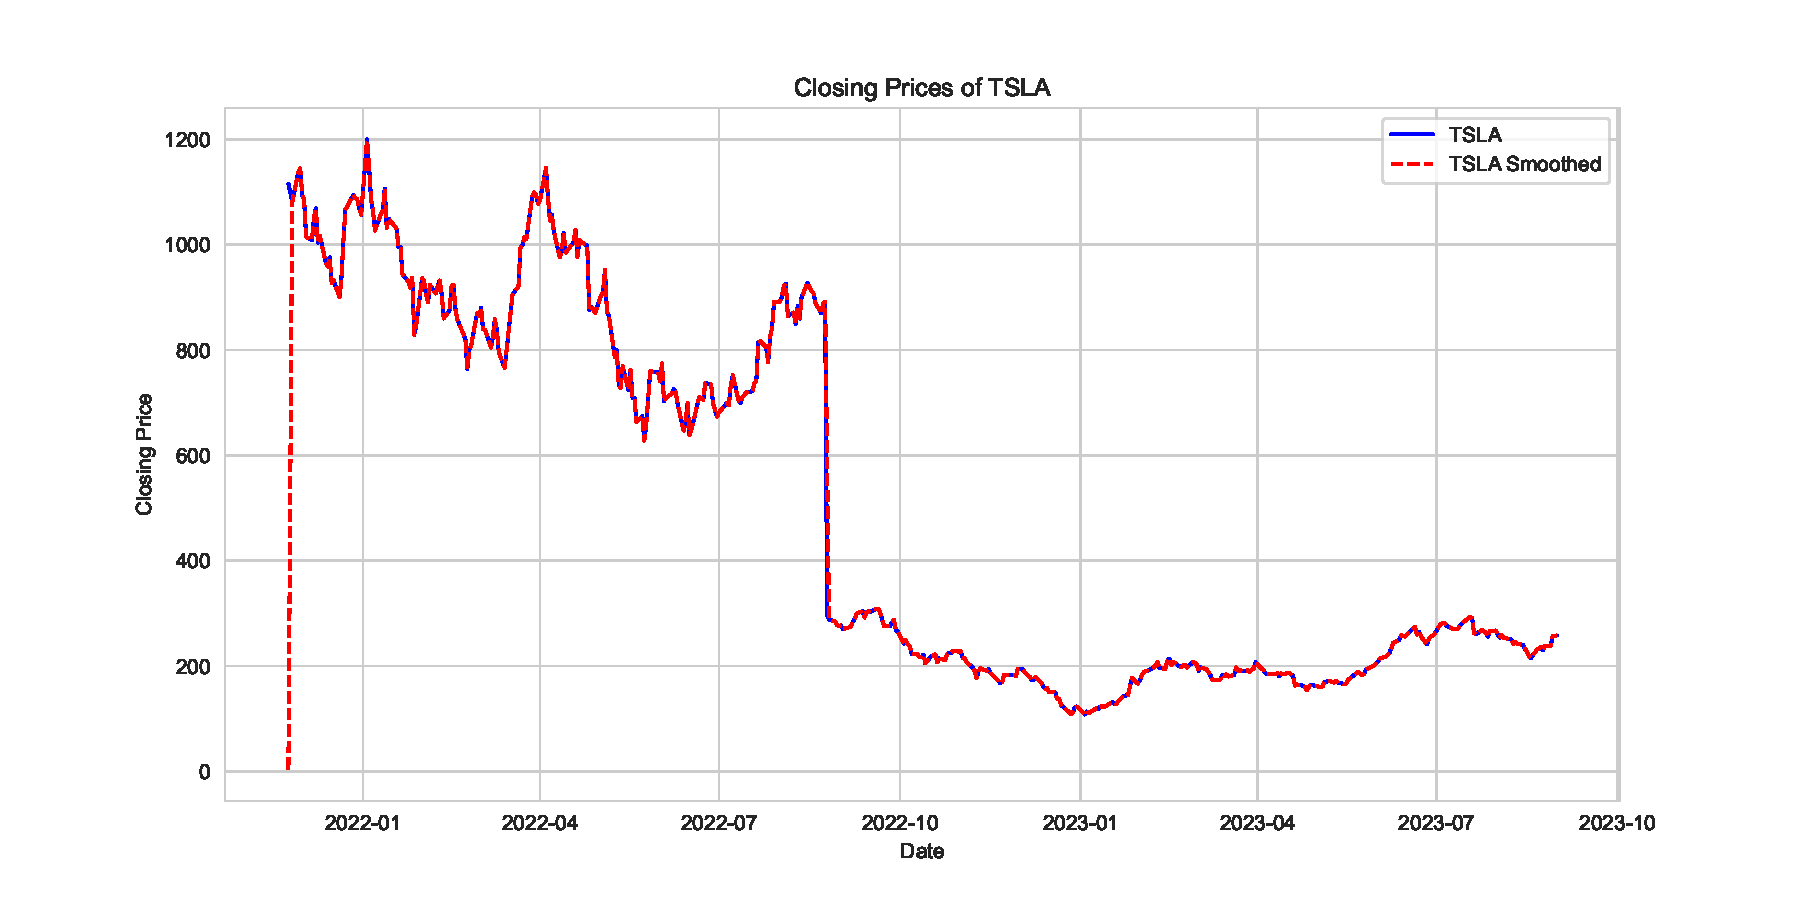
\includegraphics[width=0.50\textwidth]{figs/ctien_split.pdf}   \\
\caption{ Stock split for Tesla.}
\label{fig:finalnw}
\end{figure}

Furthermore, we focus on monitoring daily changes in interaction with various markets. Consequently, we calculate these changes as daily  \textit{logarithmic returns} for several reasons. The most significant one is that a stock market can be modelled using a geometric Brownian motion. This allows us to apply \textit{It\^{o}'s lemma}\footnote{It\^{o} calculus is beyond the scope of this thesis, but is a recommendation for interested readers and enthusiasts for stochastic calculus.} to obtain a log-normal distribution. As we aim to achieve normally distributed variables, we utilise the natural logarithm. Additionally, our approach normalises the data set. \cite{Joshi2008} \cite{Hull2021}
Also for general purposes the overall data set has been normalised. This will be demonstrated in the results.
For better comparability and explain-ability a random number has been added. It is constructed once and not changed for each seed. This is an important step for the upcoming sensitivity analysis as an benchmark of noise.
To ensure the data is in the correct order, it is sorted by date and symbol.
The last step is separating the training data from the testing data with a split of 80/20.

\subsubsection{Noise reduction} %Jonas
Unfortunately, financial data is noisy and possesses a low signal-to-noise ratio  which makes it difficult to use as a basis for machine learning. \cite{Prado2018, Hull2021} One solution to overcome this problem as described in \cite{Li2022}  is to use technical indicators to stabilise the state due to their inherent characteristic of a rolling window. 
\chapquote{``Technical indicators can reflect the changes in the stock market \newline from different perspectives and reduce the influence of noise."}{\textsc{Li}}{\cite[p. 1]{Li2022}}
Hence, they are added to the data set. But this is only the first step to improve our signal-to-noise-ratio. Our market data of current stock prices can be described as \enquote{a small bird flying through dense jungle foliage at dusk}\cite[p. 497]{Russell2021}. You only notice short, interrupted flashes of movement, which you use to guess the birds current and next position so that you won't loose it. This is the intuition behind the optimal Bayesian filter -- the Kalman Filter -- which estimates time dependant state variables from noisy observations. This can be the position and velocity of a bird or our stock prices. Without going into too much detail, the Kalman filter works iterative. 

\begin{figure}[h]
\centering
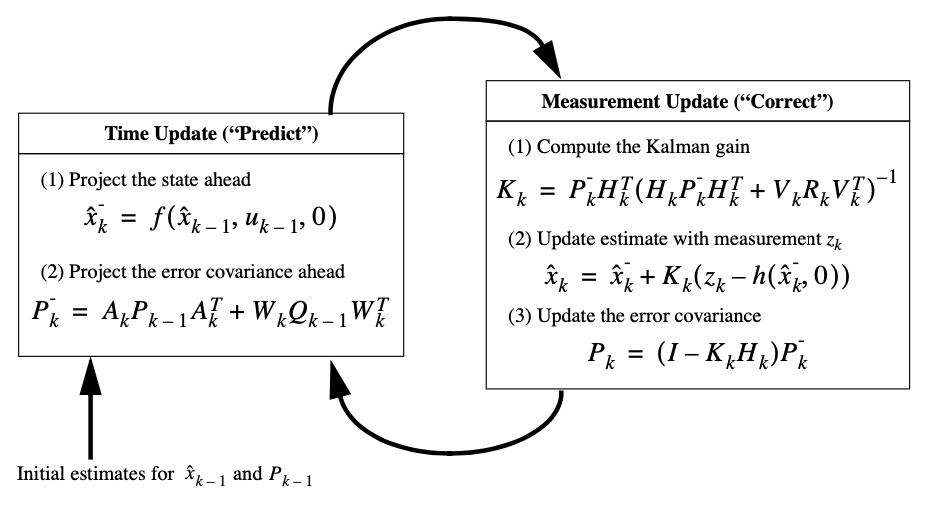
\includegraphics[width=0.75\textwidth]{figs/KalmanProcess.png}   \\
\caption{ Recursive Process of predict and correct. \cite[p. 6]{Welch1994}}
\label{fig:finalnw}
\end{figure}
The first step is the initialization where the state and belief of the filter is initialized.
The other two steps are recursive: predict and correct.
Based on the past data, the state of the next time step is predicted and the belief is adjusted to account for uncertainty.
For the update, the actual measurement and its associated belief about the accuracy are used to calculate the probability of both the measurement and prediction. Depending on those probabilities a state between both of them is adapted as "true" measurement and the belief in its accuracy is updated. This iterative process is superior to basic smoothing algorithms as it leverages the probabilities of outliers. However, the run time is extremely high. \cite{Welch1994, Russell2021, Labbe2020}
  

\begin{figure}[h]
\centering
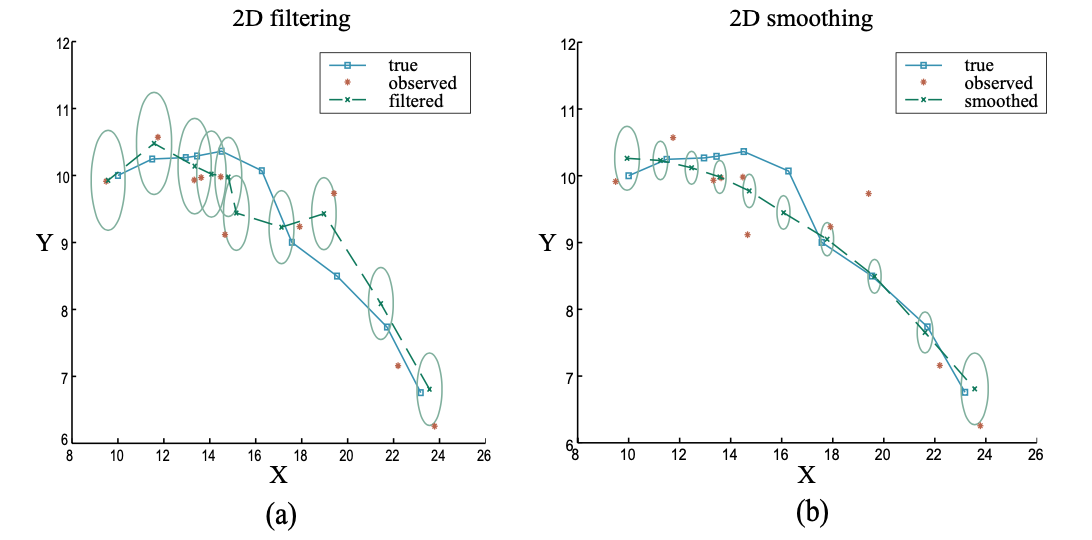
\includegraphics[width=0.9\textwidth]{figs/plotKalman.png}   \\
\caption{Results of Kalman filtering (a) and smoothing (b) for an arbitrary  object. The true position, it's actual noisy measurements and the estimated states of the filter are displayed. Ovals are indicating the variance in the position estimates. \cite[p. 502]{Russell2021}}
\label{fig:finalnw}
\end{figure}




\section{RL Approach: FinRL}
\label{subsec:FinRl}
FinRL is a framework designed for research in the field of reinforcement learning within the context of finance and trading. It is constructed upon the OpenAI Gym framework and is designed to simulate real stock markets using actual data. The aim of FinRL is to provide easy accessibility to this domain by offering various environments and fine-tuned Deep Reinforcement Learning (DRL) agents, among other resources \cite{liu2020finrl}.
Figure \ref{fig:FinRL-structure} illustrates the structure and various functionalities of the FinRL library.
\begin{figure}[h]
    \centering
    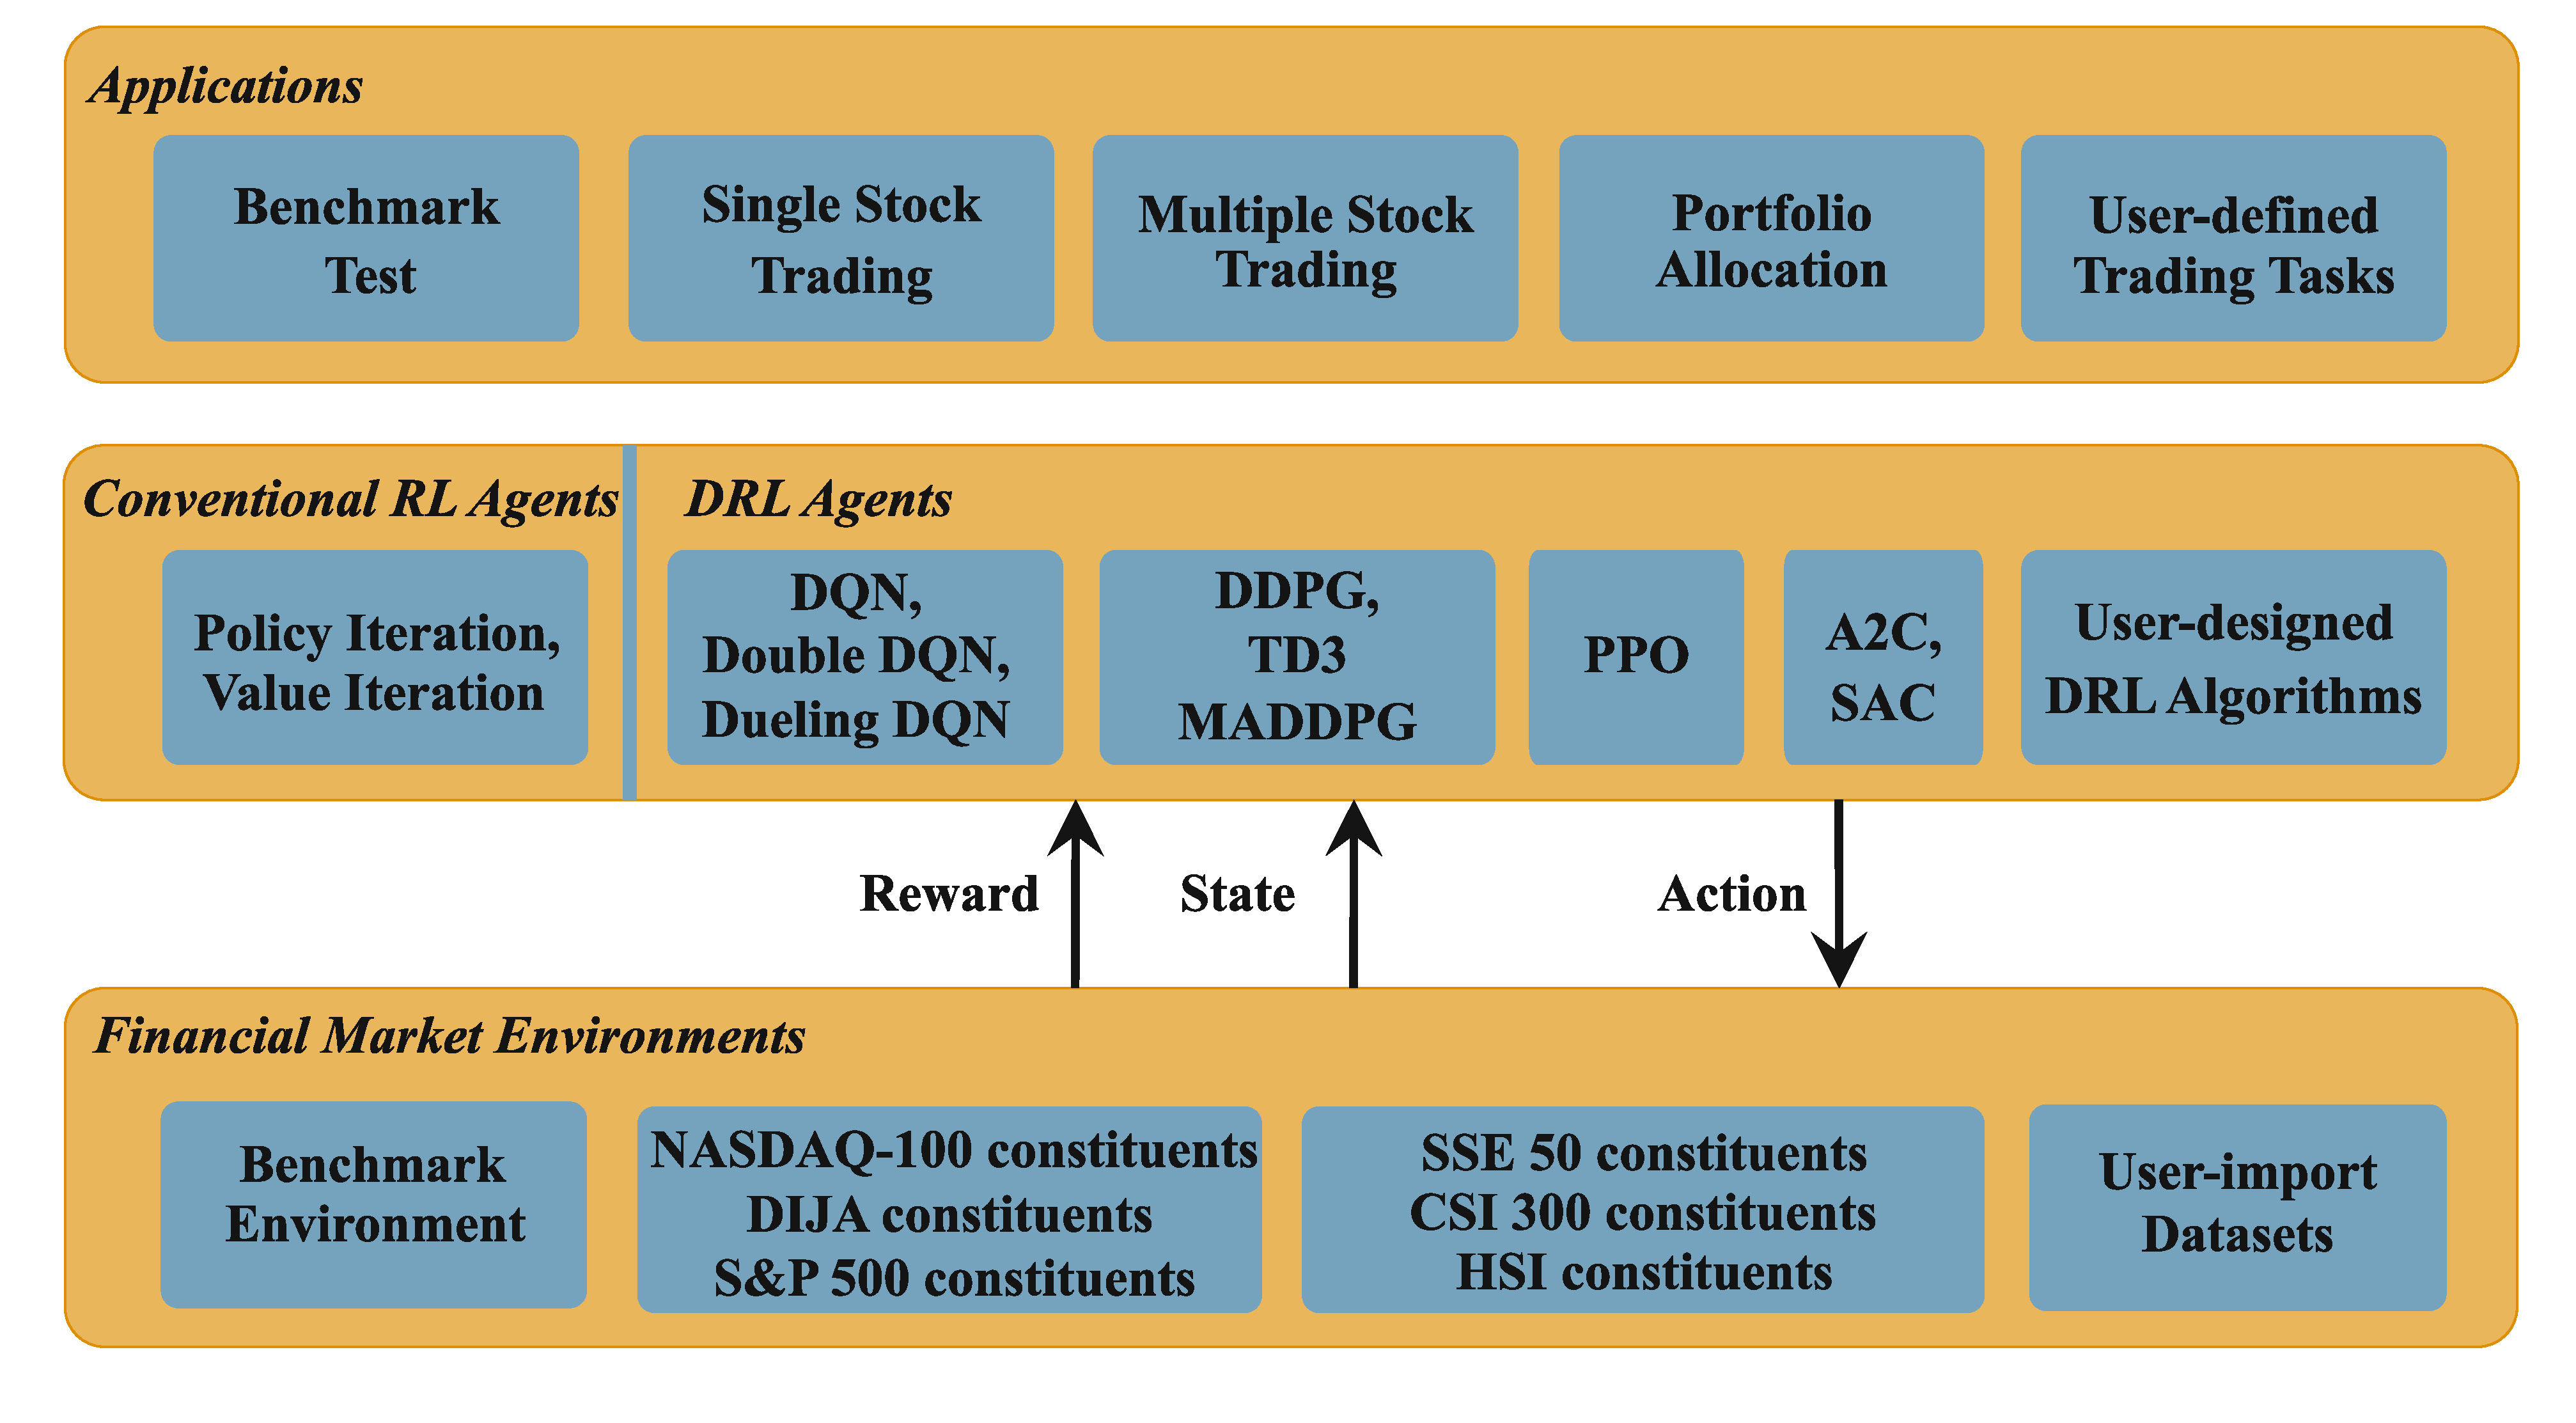
\includegraphics[width=0.85\textwidth]{figs/FinRl_structure2.pdf}
    \caption{Structure of the FinRL Framework with visualization of options among three main modules \cite{liu2020finrl}.}
    \label{fig:FinRL-structure}
\end{figure}
In this thesis, we have opted for the application of single-stock trading using the implemented agents A2C, DDPG, PPO, TD3, SAC, and have leveraged the opportunity to employ our own dataset.

%\subsection{State (Lorena)}%Lorena


\subsection{Environment} %Lorena
\label{subsubsec:env}

The foundation for the environment used in this research is based on the FinRL Stock Trading Environment, which was modified to meet our specific requirements.
As FinRL follows the OpenAI gym-style, every environment provides the functions \texttt{reset()}, \texttt{step()} and \texttt{reward()}. As the name \textit{reset} implies, this function resets the environment, returning it to its initial state, \texttt{step()} takes an action from the environment and updates the state and \texttt{reward()} calculates the corresponding reward for the performed action \cite{liu2022finrlMeta}. For stock trading, it is essential to have functions for buying and selling stocks. The former must assess how much budget is available for purchasing, taking into account transaction fees. The latter function has to check how many of the stocks to be sold are owned, ensuring that it does not sell stocks that are not in possession. If a turbulence threshold is provided, it is examined whether the turbulence indicator exceeds this threshold, as a high turbulence index corresponds to a heightened risk of a stock market crash. If the turbulence index surpasses the provided threshold, buying is stopped and all stocks are sold \cite{liu2020finrl}.
The interface between the agent and the environment is the state space which is defined in the environment. Therefore functions to initiate and update the state are provided.  

In the original environment, the state consists of the available budget, the price of each stock at the current timestep, the portfolio, i.e. how many stocks we own from each stock and all technical indicators. A graphic illustrating the state can be found in Figure \ref{fig:oldState}.

\begin{figure}[h]
    \centering
    
\includegraphics[width = 0.65\textwidth]{figs/old_state.pdf}
    \caption{Original state provided by the FinRL Stock Trading Environment. It consists of the current budget, the prices for each stock, the number of stocks owned of each stock and the technical indicators for each stock. }
    \label{fig:oldState}
\end{figure}

The first modification made to the environment was the addition of a sentiment list to the state, following the example of technical indicators. This allows providing the agent with additional sentiment data for decision-making. As in Section \ref{subsec:dataPre} elaborated it is useful to use daily changes instead of absolute prices. Replacing the absolute prices seemed less logical due to their necessity in calculations related to potential purchase quantities. Therefore, the rate of change was incorporated as additional information into the state. The literature highlights a correlation between stock prices and trading volume, making it sensible to include volume in the state as well \cite{campbell1993trading}\cite{gallant1992stock}. Overall, a graphic illustrating the state of the modified environment can be found in Figure \ref{fig:newState}.
Hereby, budget is of size one, the price-block is as big as the number of stocks which is also the case for the portfolio block as well as for the daily change rate and the traded volume. The technical indicator part is of size $number of technical indicators \cdot number of stocks$ and the sentiment data part is of size $ number of sentiment data \cdot number of stocks$.  
As we are using 30 stocks that can be traded by the agent our state is of size 421 when not using sentiment data and of size 541 when including sentiment data. 
As this is already a state of big dimension, the plan of adding more than one timestep or more alternative or fundamental data had to be rejected.


%\textcolor{red}{State always one single timestep --> thought about adding more, but the dimensions where too high. Also the plan to add more alternative or fundamental data had to be rejected.}

\begin{figure}[h]
    \centering
    
\includegraphics[width=0.95\textwidth]{figs/new_Sate.pdf}
    \caption{Modified state consisting of the same components as the original state and additionally sentiment data for each stock, the change rate and the traded volume of each stock. }
    \label{fig:newState}
\end{figure}

 The original environment was designed exclusively for the use of daily data, which necessitated several adjustments to accommodate hourly data processing, including the calculation of the Sharpe ratio. 
 The final modification made pertained to the seeding of the random function. To enhance result reproducibility, the seed is now provided within a range from zero to $n$. Consequently, the seed function in the environment had to be adjusted to meet this requirement. It involves passing the current seed to the environment, which then utilizes it to seed its random function.
 

\subsection{Agents}%Mohamad
\label{subsubsec:agents}
Stable Baselines3 is a widely used library for training and evaluating reinforcement learning agents. It offers state-of-the-art algorithms, providing users with practical tools for their RL tasks \cite{stable-baselines3}. Our study involved 50,000 timesteps for each of the agents we used from the Stable Baselines3 library. Here is an overview of those agents:
\begin{itemize}
\item \textbf{A2C (Advantage Actor-Critic)}: A synchronous, deterministic variant of Asynchronous Advantage Actor-Critic (A3C) \cite{mnih2016asynchronous}.

\textbf{Parameters}: We've employed the standard model provided by the FinRL Stable Baselines3 library without any modification to the default parameters.
\item \textbf{PPO (Proximal Policy Optimization)}: An on-policy algorithm which aims to alleviate issues related to large policy updates \cite{schulman2017proximal}.

\textbf{Parameters}:
\textit{n\_steps:} 2048 - The number of steps to run for each environment per update.
\textit{ent\_coef:} 0.01 - Entropy coefficient for exploration.
\textit{learning\_rate:} 0.00025 - The learning rate of the optimizer.
\textit{batch\_size:} 128 - Size of the batches for learning.
\item \textbf{SAC (Soft Actor-Critic)}: An off-policy actor-critic deep RL algorithm based on the maximum entropy reinforcement learning framework \cite{haarnoja2018soft}.

\textbf{Parameters}:
\textit{batch\_size:} 128 - Size of the batches.
\textit{buffer\_size:} 100,000 - Size of the replay buffer.
\textit{learning\_rate:} 0.0001 - The learning rate of the optimizer.
\textit{learning\_starts:} 100 - Number of steps before starting training.
\textit{ent\_coef:} "auto\_0.1" - Coefficient for the entropy regularizer, with automatic tuning.

\item \textbf{TD3 (Twin Delayed Deep Deterministic Policy Gradient)}: An algorithm that addresses function approximation errors in DDPG \cite{fujimoto2018addressing}.

\textbf{Parameters}:
\textit{batch\_size:} 100 - Size of the batches.
\textit{buffer\_size:} 1,000,000 - Size of the replay buffer.
\textit{learning\_rate:} 0.001 - The learning rate of the optimizer.

\item \textbf{DDPG (Deep Deterministic Policy Gradient)}: A model-free, off-policy, actor-critic algorithm \cite{lillicrap2019continuous}.

\textbf{Parameters}: We've utilized the standard model from the FinRL Stable Baselines3 library without adjusting any default parameters.

Each of these agents brings unique advantages to different scenarios, and their performances can be contingent upon both the nature of the task and the specific parameter configurations used.
\end{itemize}

\section{Sensitivity Analysis} %Viktoria
\label{subsec:sensitvity}
%Vorgehen (Export der Policy als ONNX Modell, transferieren in Tensorflow Modell, anwenden des Gradient Tapes)
In our project, we opted for the gradient-based method for sensitivity analysis. Our decision was primarily influenced by two key attributes of this method: its simplicity and generalizability \cite{gradients_tutorial}. The gradient-based method offers a straightforward approach to understanding how changes in input variables can influence the output of a model. By computing the gradient of the output with respect to the input, we can directly measure the model's sensitivity to each input variable. This method is not only intuitive but also generalizable across various types of models and datasets.

To facilitate this analysis, we employed the TensorFlow Python Library \cite{tensorflow2015whitepaper}, a powerful tool renowned for its capabilities in deep learning and gradient computations. With TensorFlow, we can efficiently compute the gradients of our model's output with respect to its inputs.

Our primary focus will be on visualizing the absolute values of these gradients. Specifically, we are interested in the gradients of features that correspond to:
\begin{itemize}
    \item \textbf{Different stocks}: This will provide insights into which stocks have the most influence on the model's predictions. By understanding the sensitivity associated with each stock, we can better gauge the importance and impact of individual stocks on our model's decision-making process.

    \item \textbf{Different days}: Analyzing the gradients across different days will allow us to discern any temporal patterns or anomalies that might exist. This can be crucial in understanding how the model's sensitivity varies over time, especially in the volatile world of finance where market dynamics can change rapidly.

    \item \textbf{Different features}: Beyond stocks and days, we will also delve into the gradients of other features, such as technical indicators and sentiment inputs, used in our model. This will shed light on which specific attributes or indicators are deemed most crucial by our model.
\end{itemize}
In summary, our gradient-based sensitivity analysis has several benefits. Firstly, it helps us understand the deeper workings of our model's decision-making process. We can determine the main factors influencing the model's predictions by visualizing and interpreting the gradients. This insight will lead to a more knowledgeable and sturdy use of our reinforcement learning model in finance.

Furthermore, this analysis helps us identify features that might not be very important, like certain technical parameters for stocks or specific sentiment data. By spotting and then leaving out these less impactful features, our model becomes more streamlined. As a result, it can make predictions faster and train more efficiently. On the other hand, by finding the most impactful features or stocks, we can give them more importance in our model. This ensures that the most crucial parts influencing our predictions are highlighted. This combined strategy of reducing unnecessary features and focusing on the important ones not only improves the model's accuracy but also makes it run more efficiently.


\section{Backtesting} %Jonas
\label{subsec:backtest}

To verify the models and rank them by their capabilities, a holistic backtesting approach is defined. The basic idea of backtesting is trading on the test data, which was separated before. The results include the total returns (corresponds to $alpha$), but also various types of other metrics, mostly focused on risk (corresponds to $beta$). To ensure that random effects are not influencing the underlying generating process, we not only repeat the training on multiple seed numbers, but also include all these models in our back-tests simultaneously. 
The most important biases to keep in mind are the survivor-ship bias of only including the companies that "survived" and are still traded on the financial markets. The look ahead bias of unconsciously allowing the model to access future data. And most importantly the optimisation bias -- the over-fitting of an model.
Also the sample selection bias is of importance: training and testing data that has been selected can include underlying trends that will not be repeated and are an anomaly.
Especially for our problem statement we have to include trading specific obstacles, like transaction costs, slippage, volume and liquidity. Slippage describes the price differences between expected price due to market data while ordering  and the final price, that is filled, during the execution of the trade.  Volume and liquidity are not relevant, since we only include the largest stocks of the S\&P500 and test with 1mn \$ of cash and a maximum of 100 units per trade.  The transaction costs and slippage are controlled in the environment by a conservative estimate of 1\% for each trade.  \cite{liu2022finrlMeta, Hull2021, Prado2018, Garita2021} 

For a fair comparison, all three dimensions of strategies, which are based on different approaches, are included: trading on classical signals, portfolio theory and buy and hold. This includes strategies based on technical indicators like RSI, Moving Average and Bollinger Bands. But also more conservative strategies like Mean Variance Optimization -- one of the standard approaches in modern portfolio theory. It calculates the variances as a measure of risk to allocate a weight for the final trade-off between risk and return. Thus the final portfolio maximizes the return per risk. Also included is the straight forward buy and hold approach, which is only allowed to hold the same stocks our RL models have been trained on. 

As the last building block further metrics have been calculated. This is based on the \texttt{PyFolio} \cite{pyfolio} package and includes risk metrics like max draw-down (describing the highest amount lost -- from peak to trough -- in a portfolio), and its matching return-per-risk metric, the calmar ratio. Also the sharp ratio gives an risk adjusted return metric: the returns above an benchmark are adjusted to its standard deviation to estimate the risk-adjusted performance.

In total this allows a holistic estimate to research an optimal trading strategy given our demands. And with these backtests, the models parameters can be optimized, and the sensitivity analysis conducted to obtain the best performing, yet still explainable models. Thus, a randomly trading model with higher excess returns ($alpha$) with identical volatility ($beta$) is not preferred over a model whose actions are transparent. 

\section{Results} %Alle zusammen FR/SA
In this section, we present the findings and outcomes of our research. The data provides insights into the patterns and implications discovered during the study.
\label{sec:results}
%Step by step plan der Experimente um bestmöglichen Vergleich zu erzielen. We further compare normalized vs non normalized, turb threshold vs non thresh trading condition realistic vs not realistic  
%explain alpha and beta
%Erklärung welche parameter optimiert wurden und wieso erst beim Finalen Modell eine extensive grid search für optimale Parameter durchgeführt wurde (zu viele unterschiedliche Modelle und Daten Kombinationen, exponentielle Runtime, naive Annahme: Daten sind ähnlich genug dass optimale Parameter auch sehr ähnlich seien müssen. Also bei gleichen Parametern ergibt sich die Vergleichbarkeit auch ohne dezidierte Grid Search Optimierung)
%Darstellung der Ergebnisse und deren Diskussion, vergleich zu Ansätzen aus der Literatur \\
%Ergebnisse und Implementierung: 4-5 Seiten

%High variance in plots--> only trading the spread (explain meaning)
%turbulance to trade in low risk days
\subsection{Optimizing Model Hyperparameters}
In the quest for optimal model performance, hyperparameter tuning is an essential step. It involves fine-tuning various parameters to find the best combination that maximizes the model's efficiency and accuracy. For our setup, we considered four primary hyperparameters:
\begin{itemize}
    \item \textbf{Data Normalization}: Neural networks often benefit from normalized data, especially when the range of input values is vast. In our raw dataset, the highest values reach up to while the lowest values dip below zero. Such a broad spread can potentially hinder the model's learning capability. To investigate the impact of normalization, we tested two agents, A2C and PPO, with both normalized and non-normalized data.

    \item \textbf{Data Smoothing}: Smoothing data can help in reducing noise and capturing the underlying trend in the data. The idea behind this is to provide the model with a clearer signal, potentially aiding in better decision-making. We evaluated the effect of data smoothing using the A2C and PPO agents.

    \item \textbf{Transaction Costs}: Introducing transaction costs can influence an agent's trading frequency. By setting a higher transaction cost (0.01) versus a lower one (0.001), we hypothesized that the agent would trade more conservatively, leading to more stable performance. The rationale is that higher costs would deter the agent from making frequent trades unless the predicted rewards are substantial.

    \item \textbf{Turbulence Threshold}: Turbulence in the stock market can lead to erratic price movements. By introducing a threshold for turbulence, we aimed to make the agent more cautious. If a stock's turbulence index exceeds this threshold, the agent refrains from buying or selling it. This strategy was designed to mitigate potential losses during highly volatile periods. We tested this approach using the A2C and SAC agents.
\end{itemize}
\subsubsection{Data Normalization}

\begin{figure}[h]
\centering
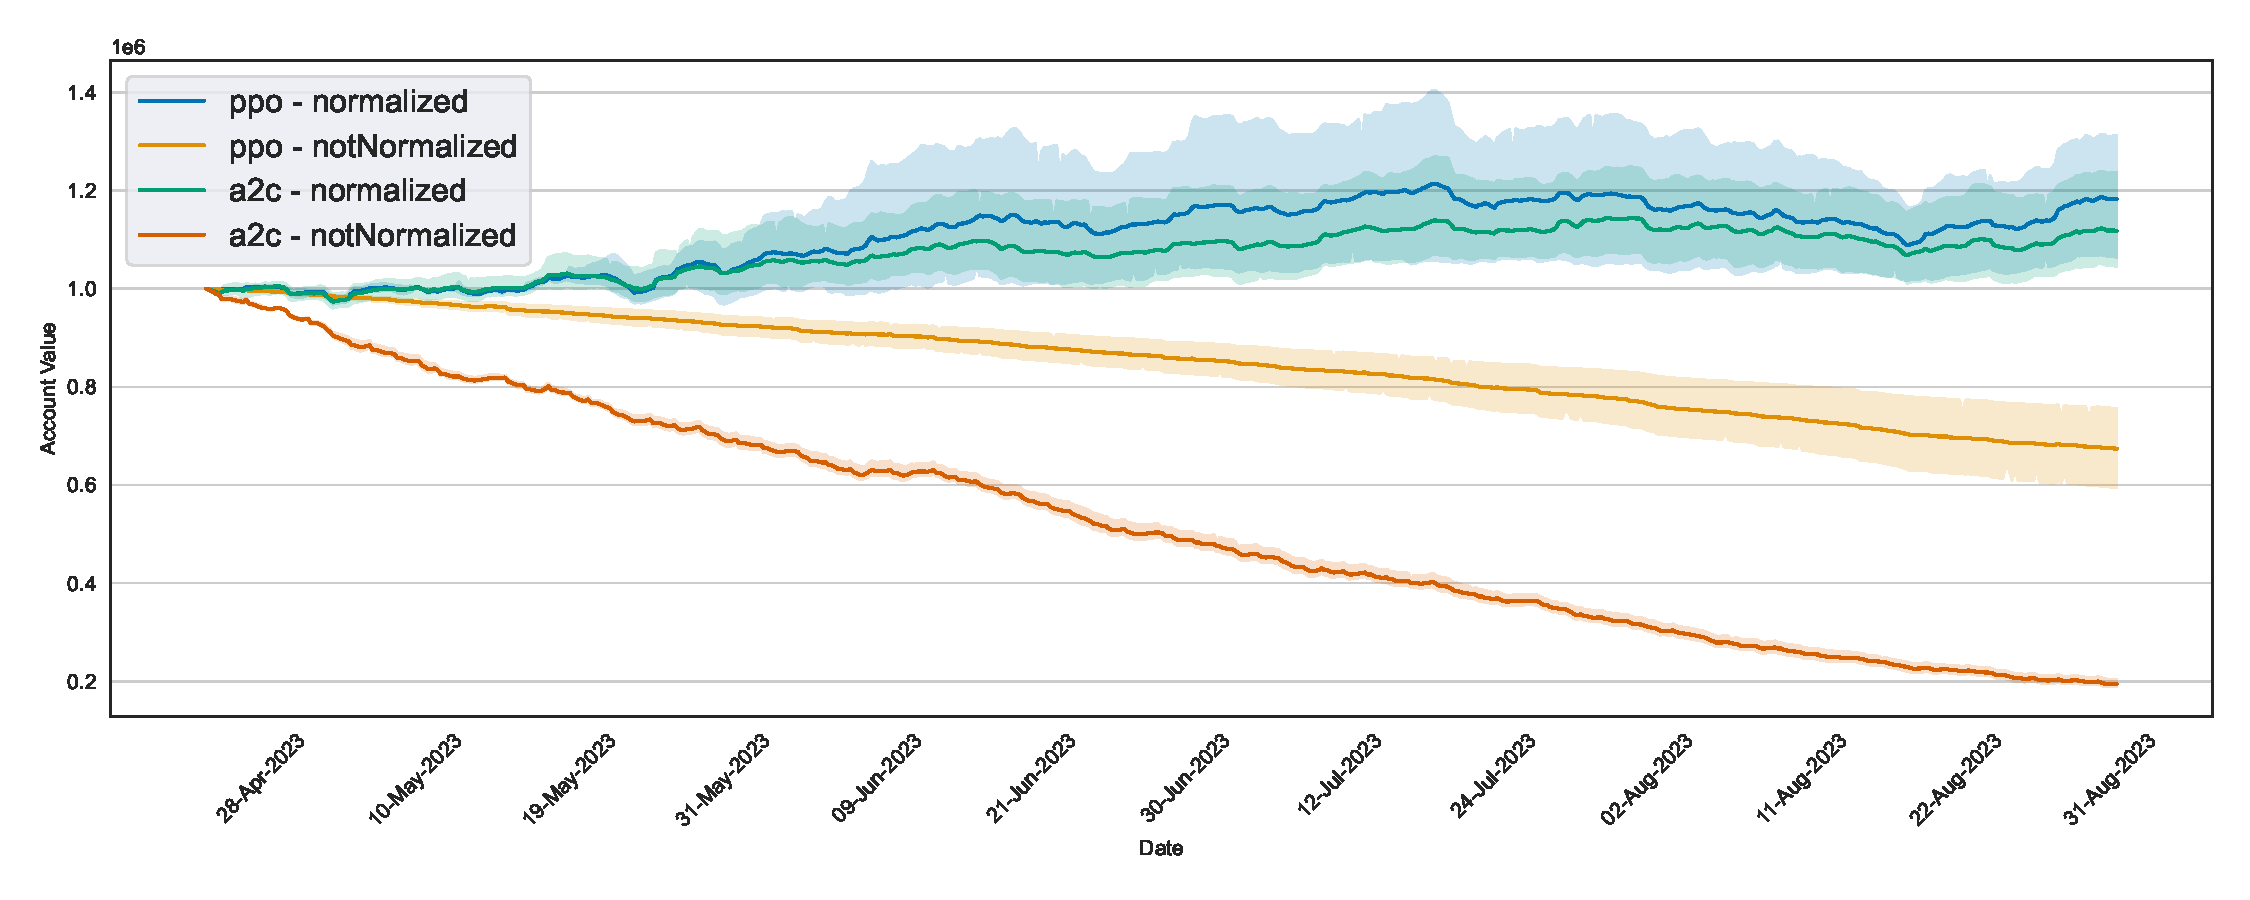
\includegraphics[width=1\textwidth]{figs/Hyperparameter_tuning/Compare_agents_performance_normalized_ppo_a2c.pdf}
\caption{Performance comparison of A2C and PPO agents with normalized vs. non-normalized data.}
\label{fig:Compare_agents_performance_normalized_ppo_a2c}
\end{figure}

Figure \ref{fig:Compare_agents_performance_normalized_ppo_a2c} offers a comprehensive visualization of the influence of data normalization on the performance of A2C and PPO agents.
In the non-normalized scenario, both agents experience a decline in account value, indicating a loss in their trading activities. This downward trajectory is almost linear, suggesting a consistent underperformance over time. Conversely, when trained with normalized data, both agents demonstrate a positive return on investment. Specifically, the A2C and PPO agents manage to achieve gains of approximately 10\% and 20\%, respectively. This stark contrast underscores the importance of data normalization in enhancing the efficency of reinforcement learning agents in stock trading.


\subsubsection{Data Smoothing}

\begin{figure}[h]
    \centering
    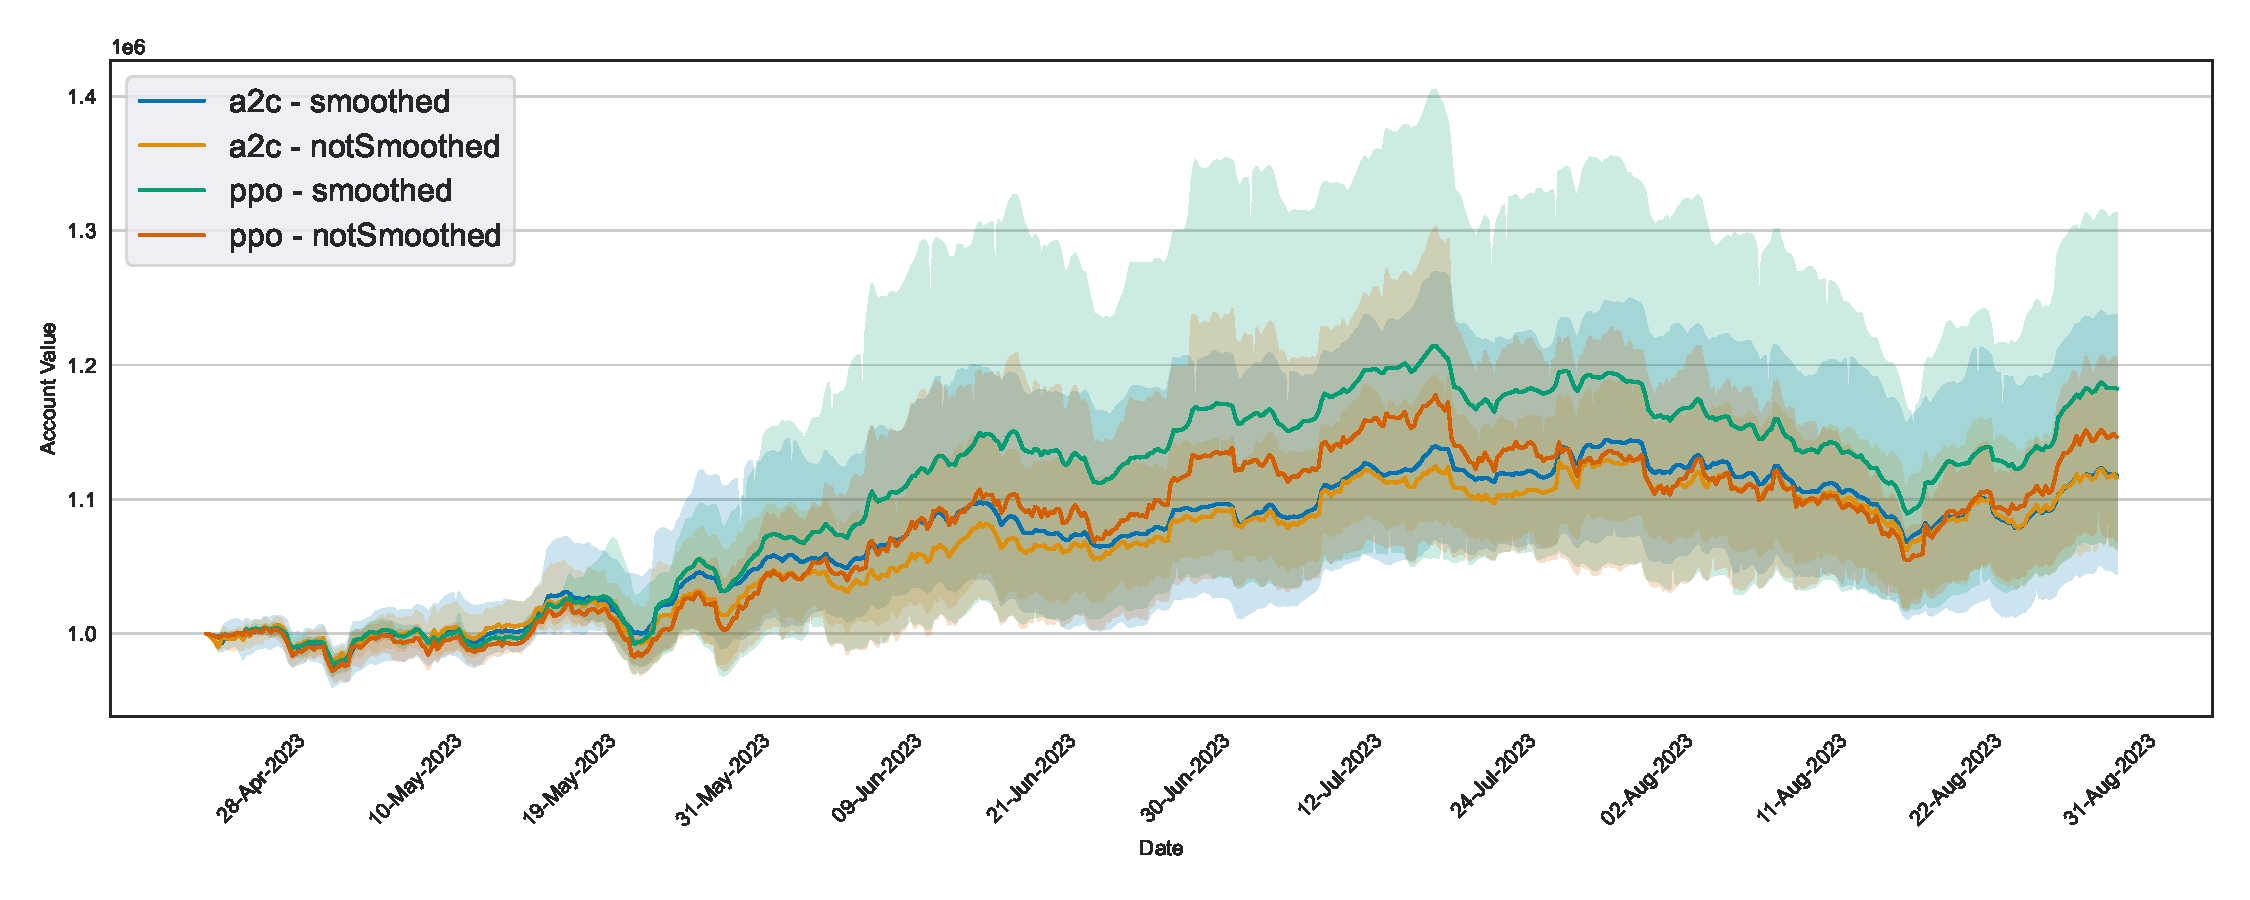
\includegraphics[width=1\textwidth]{figs/Hyperparameter_tuning/Compare_agent_performance_smoothed_a2c_ppo.pdf}
    \caption{Performance comparison of A2C and PPO agents trained on smoothed versus non-smoothed data.}
    \label{fig:Compare_agent_performance_smoothed_a2c_ppo}
\end{figure}

In Figure \ref{fig:Compare_agent_performance_smoothed_a2c_ppo} it is proven that both A2C and PPO agents trained on smoothed data outperform their counterparts trained on non-smoothed data. This suggests that employing a Kalman filter for noise reduction, thereby smoothing the data, can be beneficial for reinforcement learning agents in stock trading.


\subsubsection{Transaction Costs}

\begin{figure}[h]
    \centering
    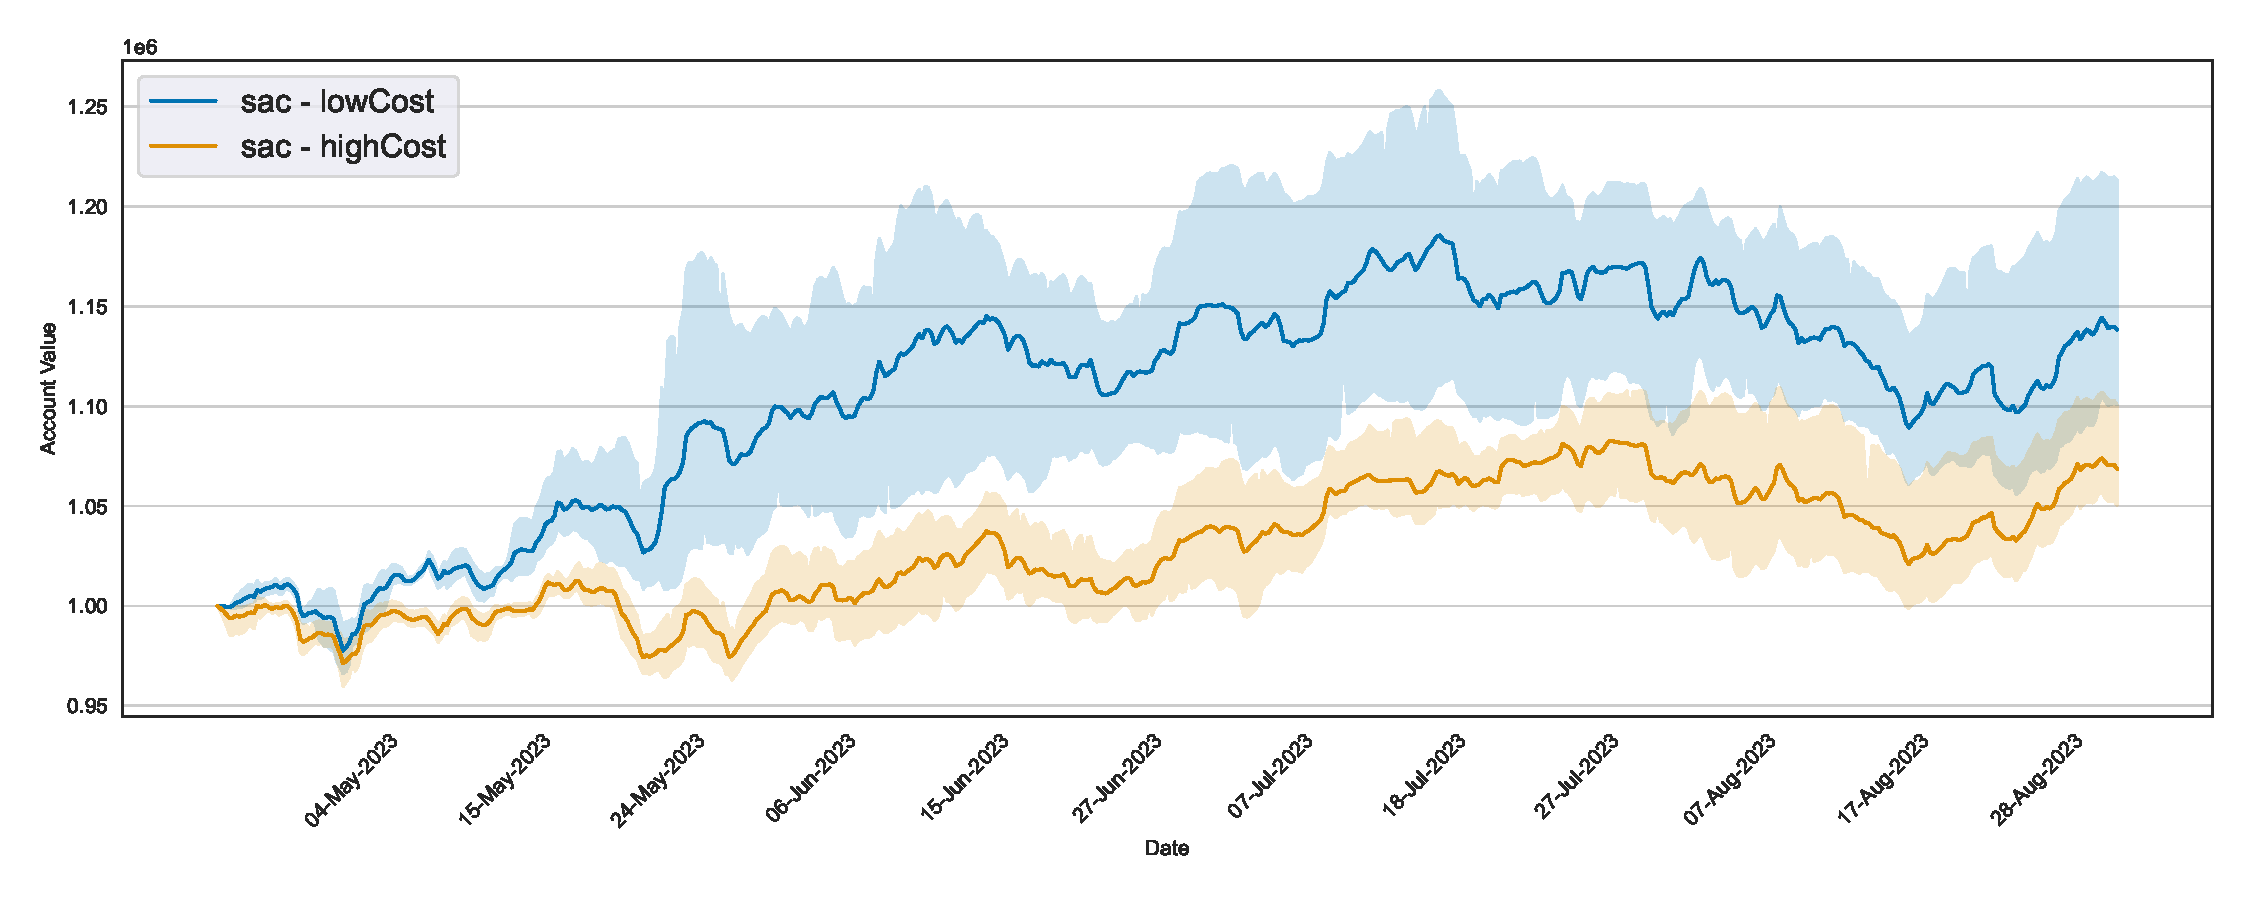
\includegraphics[width=1\textwidth]{figs/Hyperparameter_tuning/Compare_agent_performance_lowTC_sac.pdf}
    \caption{Performance comparison of the SAC agent under varying transaction costs.}
    \label{fig:Compare_agent_performance_lowTC_sac}
\end{figure}


In Figure \ref{fig:Compare_agent_performance_lowTC_sac} it is shown that both SAC agents manage to generate profits - regardeless of the transaction cost settings. However, there are clear distinctions in their trading behaviors. The agent trained with low transaction costs tends to fully utilize its capital to purchase stocks, resulting in a higher final account value. Yet, this aggressive trading strategy comes at a cost: its performance exhibits a standard deviation that is five times larger than that of the agent trained with higher transaction costs. This heightened volatility suggests a less stable trading behavior. Given the importance of stability and predictability in stock trading, we opted for the higher transaction costs setting to ensure a more consistent and reliable performance from our agent.

\subsubsection{Turbulence Threshold} 
\begin{figure}[h]
    \centering
    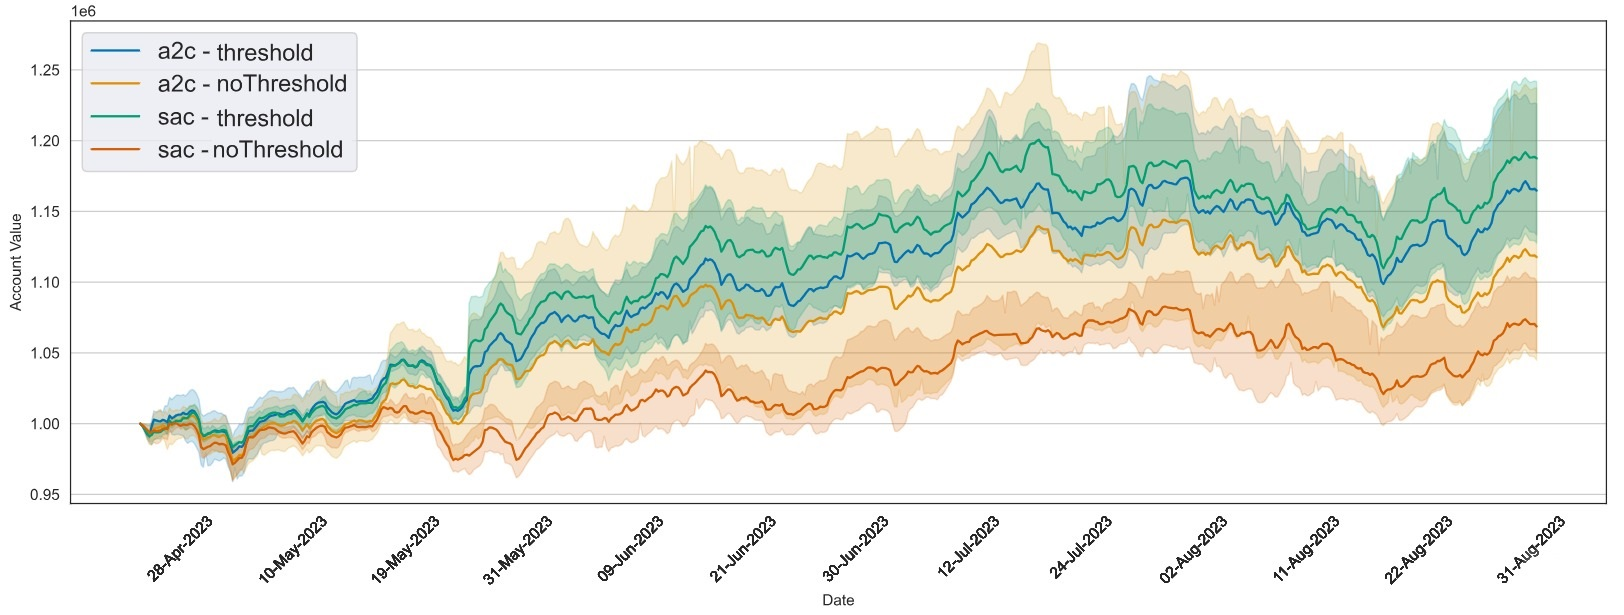
\includegraphics[width=1\textwidth]{figs/Hyperparameter_tuning/Compare_agents_performance_threshold_sac_a2c.jpg}
    \caption{Performance comparison of A2C and SAC agents with and without setting a turbulence threshold.}
    \label{fig:Compare_agents_performance_threshold_sac_a2c}
\end{figure}

Figure \ref{fig:Compare_agents_performance_threshold_sac_a2c} illustrates a clear performance distinction between agents trained with setting a turbulence threshold and those without. Both A2C and SAC agents exhibit superior performance when utilizing the turbulence threshold. Moreover, the agents without the turbulence threshold demonstrate a higher deviation, indicative of their unstable trading behavior. Given the evident benefits of stability and improved performance, we opted to incorporate the turbulence threshold in our subsequent experiments.

\subsection{Evaluating the Impact of Sentiment Data Integration}

\begin{figure}[h]
    \centering
    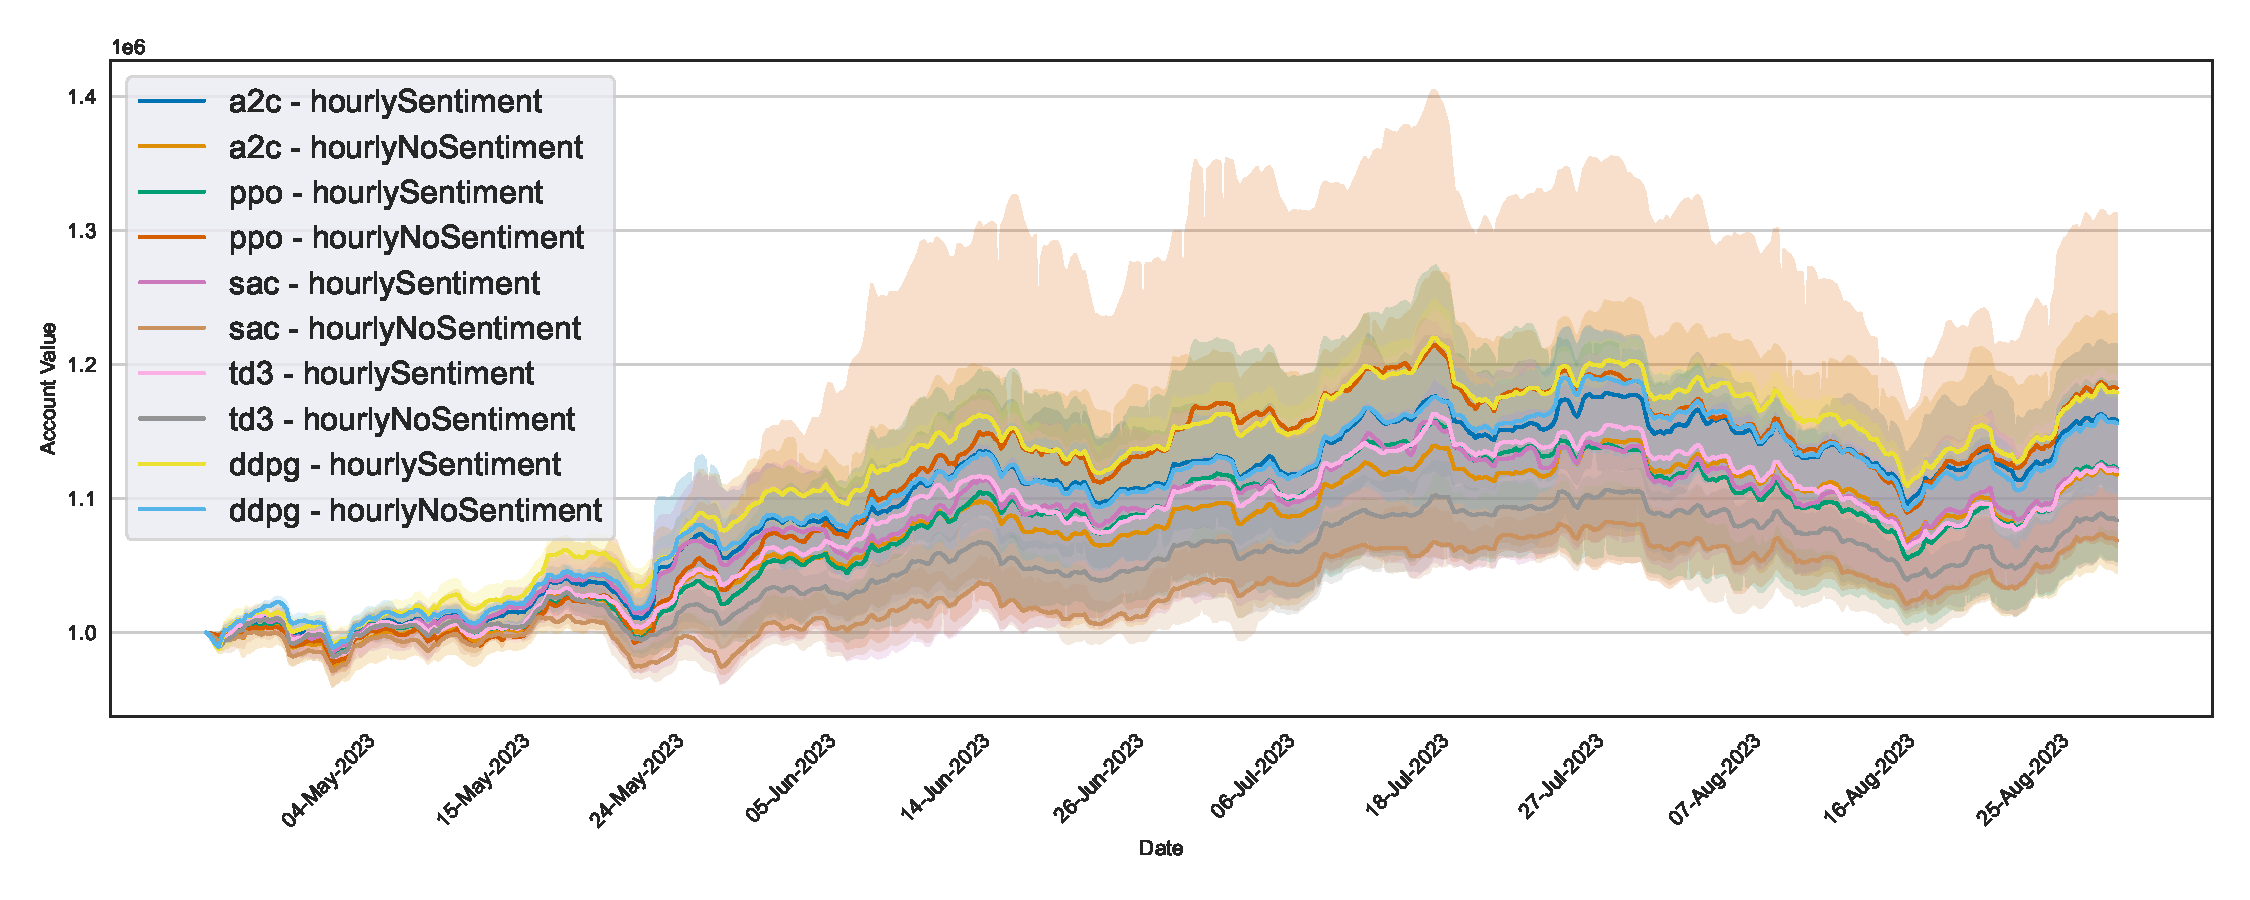
\includegraphics[width=1\textwidth]{figs/Models_comparison/Compare_agent_performance_hourlySentiment_a2c_ppo_sac_td3_ddpg.pdf}
    \caption{Performance comparison of agents trained with hourly data, with and without sentiment integration.}
    \label{fig:Compare_agent_performance_hourlySentiment_a2c_ppo_sac_td3_ddpg}
\end{figure}

\begin{figure}[h]
    \centering
    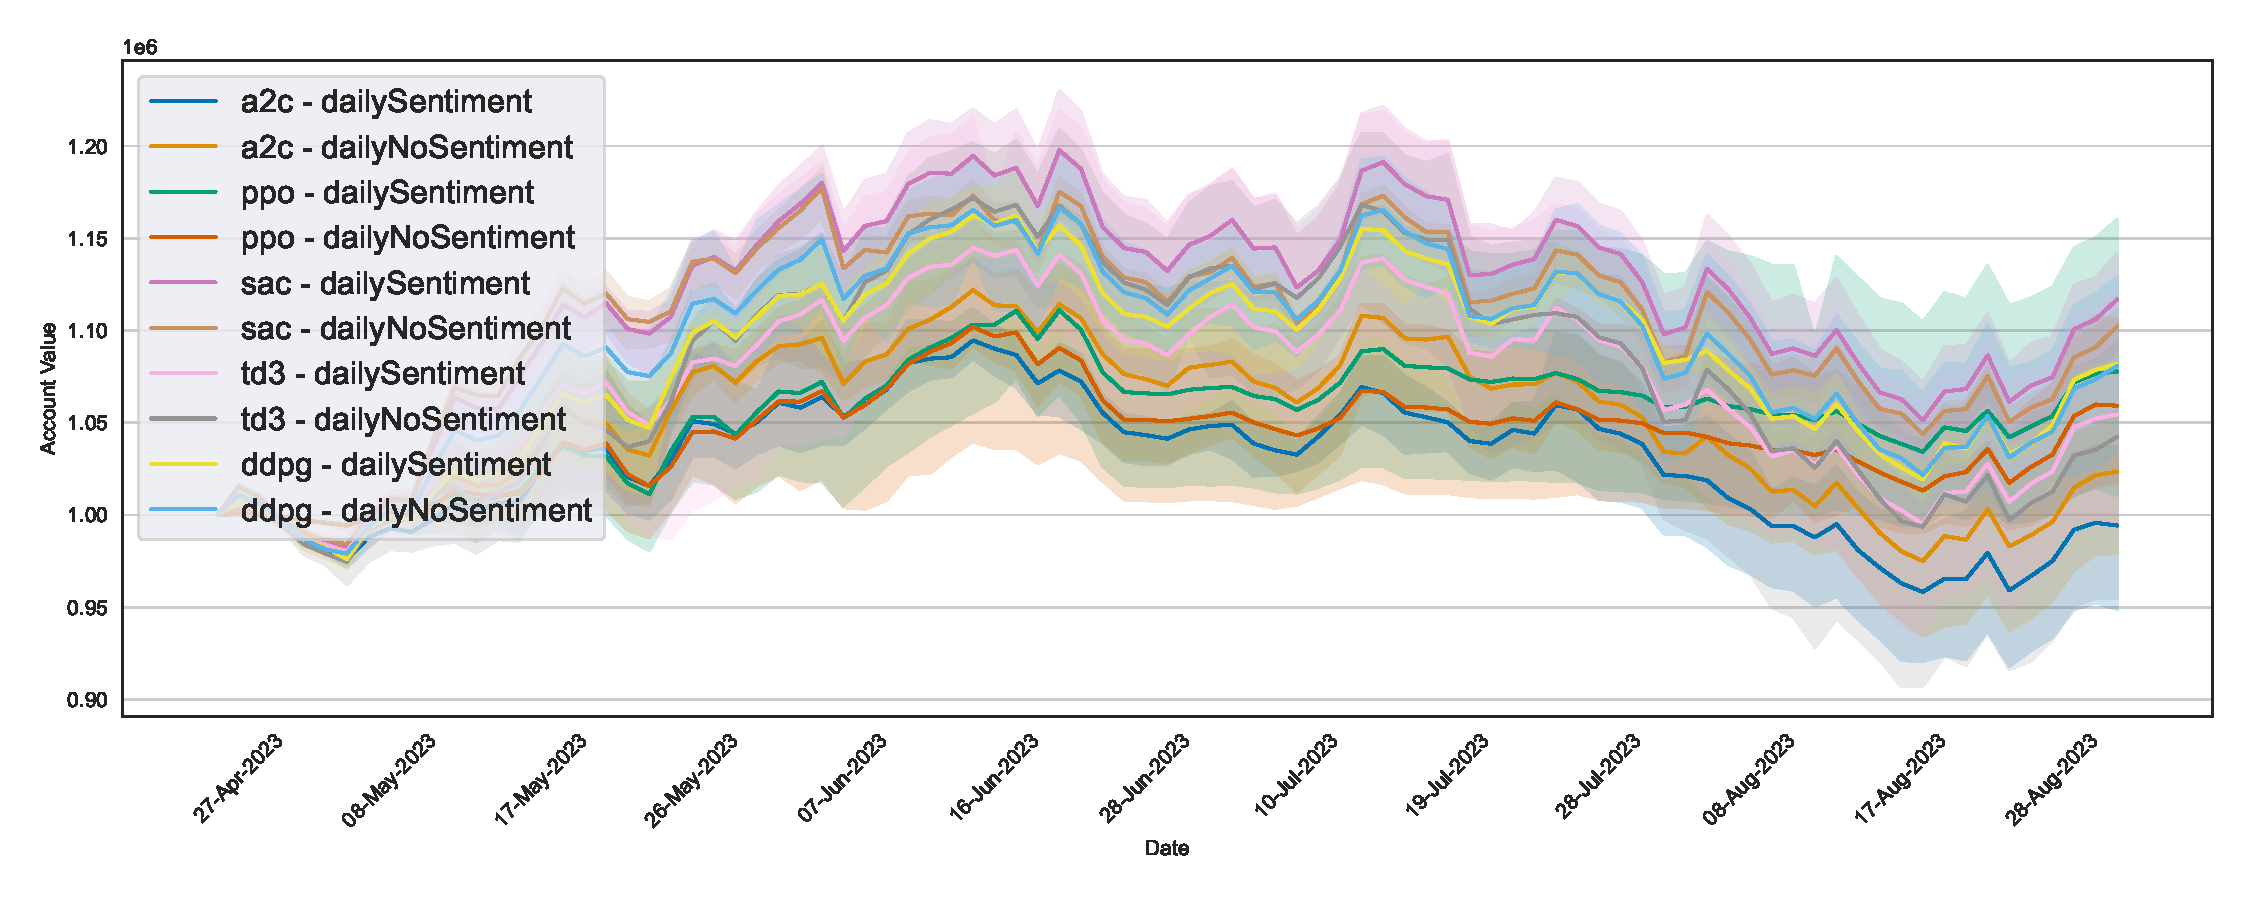
\includegraphics[width=1\textwidth]{figs/Models_comparison/Compare_agent_performance_dailySentiment_a2c_ppo_sac_td3_ddpg.pdf}
    \caption{Performance comparison of agents trained with daily data, with and without sentiment integration.}
    \label{fig:Compare_agent_performance_dailySentiment_a2c_ppo_sac_td3_ddpg}
\end{figure}

From Figures \ref{fig:Compare_agent_performance_dailySentiment_a2c_ppo_sac_td3_ddpg} and  \ref{fig:Compare_agent_performance_hourlySentiment_a2c_ppo_sac_td3_ddpg} it is evident that agents trained on a dataset including sentiment data consistently outperform those trained without sentiment data, irrespective of whether the data is hourly or daily. This underscores the potential value of integrating sentiment data into the training process, suggesting that sentiment provides crucial insights that enhance the predictive capabilities of the agents.

For a detailed pairwise comparison of each agent's performance, considering both daily and hourly data, with and without sentiment integration, please refer to the appendix.


\subsection{Comparing Daily and Hourly Data Models}
It's important to note that the time scales for hourly and daily data are inherently different, making a direct comparison between the two challenging. However, when we evaluate the end account values of the agents, a discernible pattern emerges. Agents trained on hourly data consistently outperform those trained on daily data. This suggests that the finer granularity of hourly data provides agents with more detailed insights, allowing them to make more informed decisions and, consequently, achieve better performance in stock trading.


\subsection{Benchmarking Against Traditional Models}

In our quest to evaluate the efficacy of our reinforcement learning agents, we benchmarked them against four classical trading strategies: Buy and Hold, Bollinger Bands, RSI, and MACD. 

\begin{figure}[h]
    \centering
    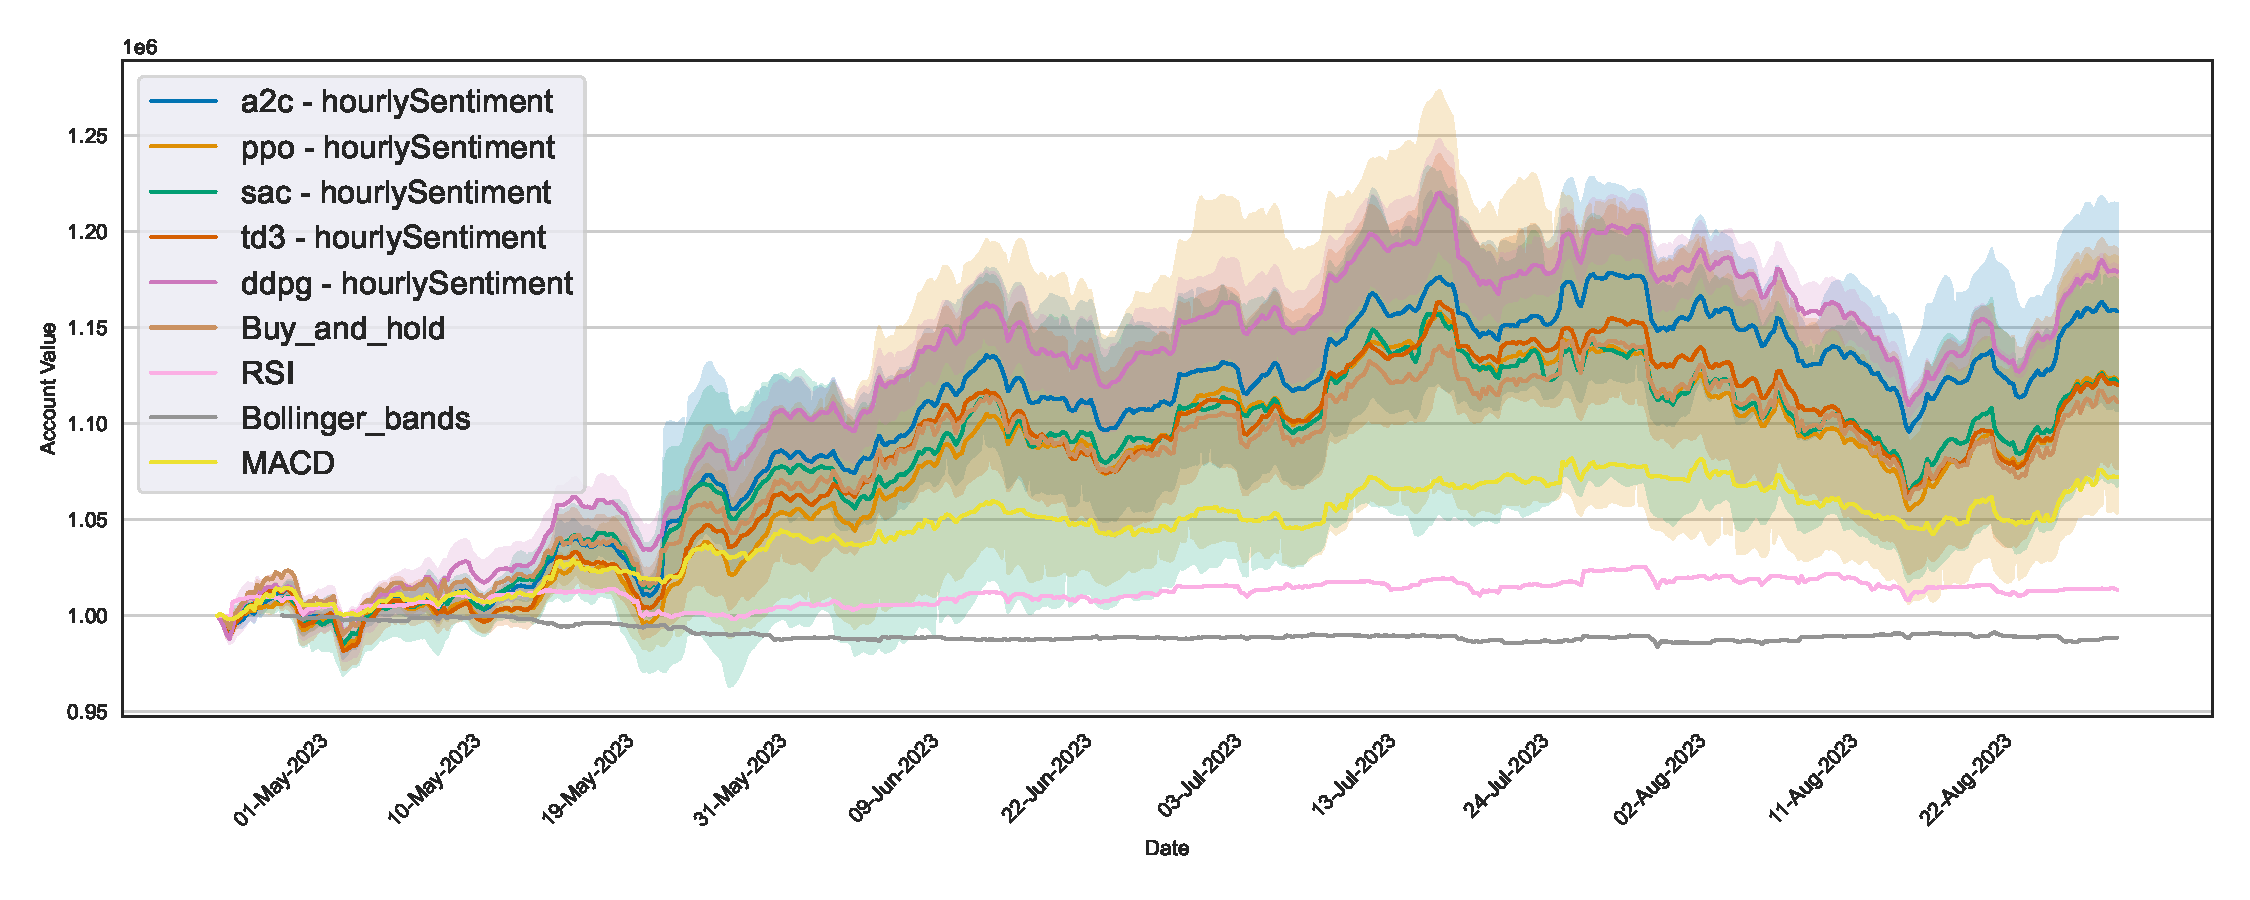
\includegraphics[width=1\textwidth]{figs/Models_comparison/Compare_agent_performance_hourlySentimentTechnical_a2c_ppo_sac_td3_ddpg_technical.pdf}
    \caption{Performance comparison of RL agents trained with hourly data against classical benchmarks. Notably, the classical benchmarks operate without transaction costs.}
\label{fig:Compare_agent_performance_hourlySentimentTechnical_a2c_ppo_sac_td3_ddpg_technical}
\end{figure}

From Figure \ref{fig:Compare_agent_performance_hourlySentimentTechnical_a2c_ppo_sac_td3_ddpg_technical}, it's evident that our RL agents consistently outperform all classical benchmarks, even when considering that the classical strategies are not burdened with transaction costs. Among the classical strategies, Buy and Hold comes closest in performance to our agents. A more detailed comparison between our agents and the Buy and Hold strategy is presented in Figure \ref{fig:Compare_agent_performance_hourlySentimentTechnical_a2c_ddpg_buy_hold}.

\begin{figure}[h]
    \centering
    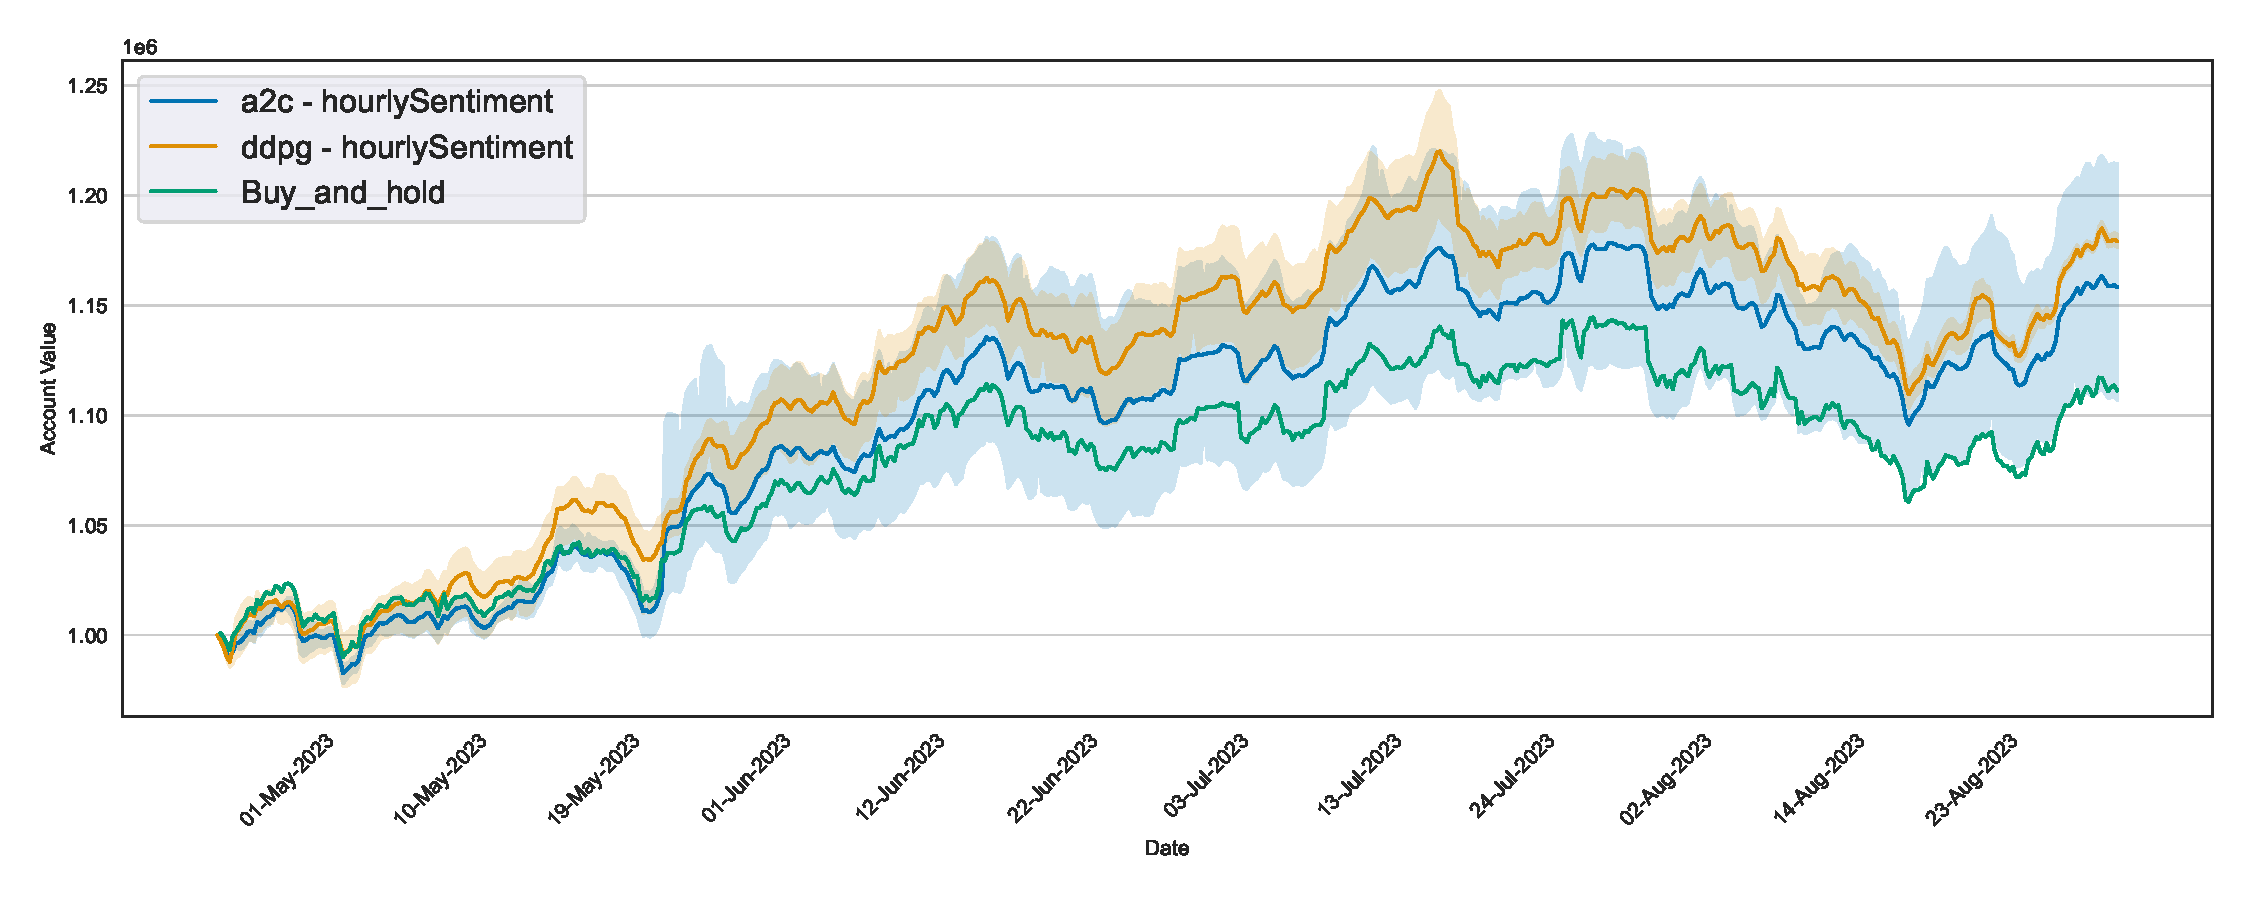
\includegraphics[width=1\textwidth]{figs/Models_comparison/Compare_agent_performance_hourlySentimentTechnical_a2c_ddpg_buy_hold.pdf}
    \caption{Performance comparison of RL agents trained with hourly data against the Buy and Hold strategy.}
\label{fig:Compare_agent_performance_hourlySentimentTechnical_a2c_ddpg_buy_hold}
\end{figure}

These results underscore the potential of RL in stock trading, indicating its ability to adapt and optimize trading strategies in a dynamic market environment, outpacing traditional, static strategies.


\subsection{Analysis of Model Sensitivity}
In this section, we present the outcomes of our comprehensive sensitivity analysis.

\subsubsection{Visualizing Gradients: A Heatmap Approach}
In our attempt to understand the model's decision-making process, we visualized the gradients using a heatmap, as depicted in Figure \ref{fig:Heatmap_hourly_SAC_random}. This heatmap represents the gradients for the Soft Actor Critic (SAC) model. A notable observation from the heatmap is the zero gradients for features in the range 330-360. At first glance, this might raise concerns about the model's functionality. However, a deeper inspection reveals that these features correspond to random numbers generated for each stock, amounting to 30 random numbers in total. The zero gradients indicate that the SAC model has effectively learned to disregard this random information, recognizing its irrelevance in the decision-making process. This behavior underscores the model's capability to discern and prioritize meaningful features, filtering out the noise or irrelevant data.

\begin{figure}[h]
    \centering
    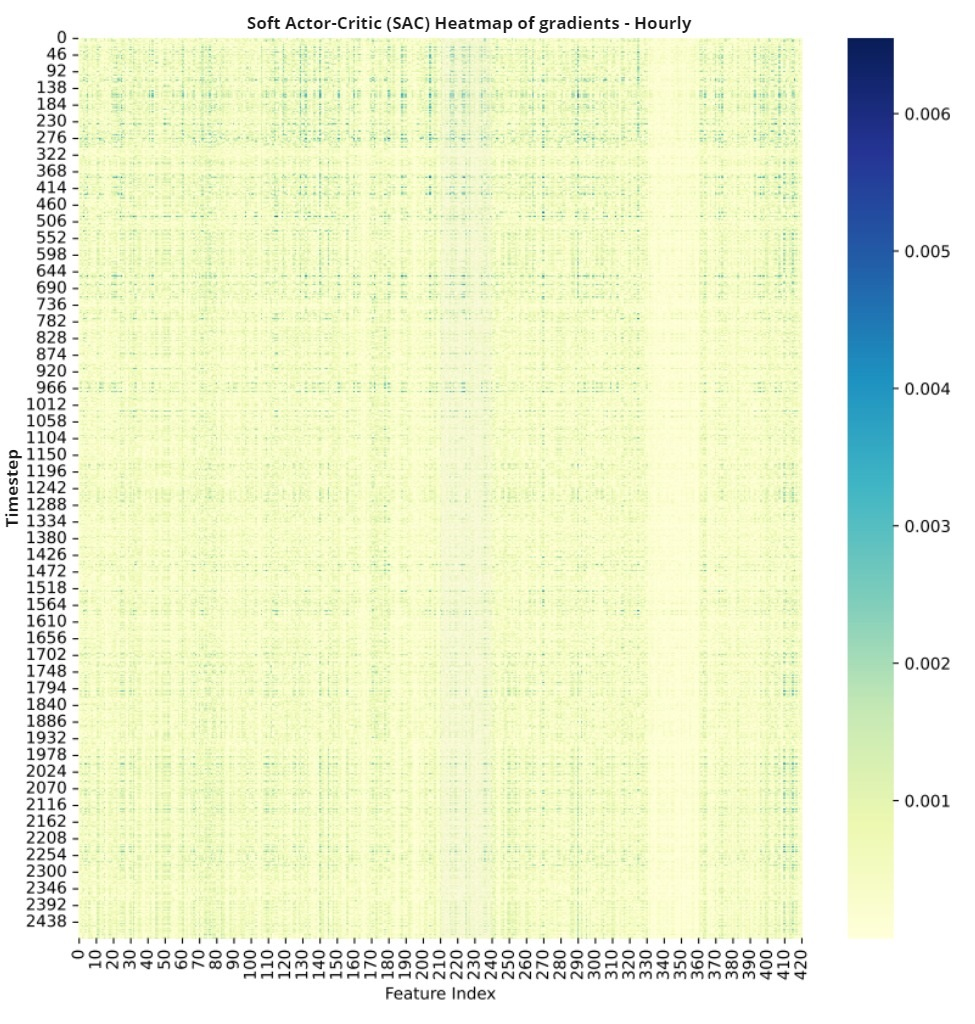
\includegraphics[width=0.8\textwidth]{figs/Heatmap_hourly_SAC_random.jpg}
    \caption{Heatmap of gradients for the SAC model: The agent tends to ignore random features (330 - 360). Additionally, one of the technical indicators (features 210 - 240, correspond to dx 30) exhibits a slightly larger gradient than others. The agent was trained on hourly data without incorporating sentiment.}

    \label{fig:Heatmap_hourly_SAC_random}
\end{figure}

Following the heatmap visualization for the SAC model trained on hourly data, we further examined the gradients for the SAC model trained on daily data, as illustrated in Figure \ref{fig:Heatmap_daily_SAC_random}. This heatmap reveals that, similar to the hourly model, the agent tends to ignore the random features (330 - 360). Interestingly, there's also a discernible pattern where the agent seems to disregard certain stocks, as represented by features 30 - 60. This behavior suggests that the model might find these specific stocks less influential or irrelevant for its decision-making process when trained on daily data.


\begin{figure}[h]
    \centering
    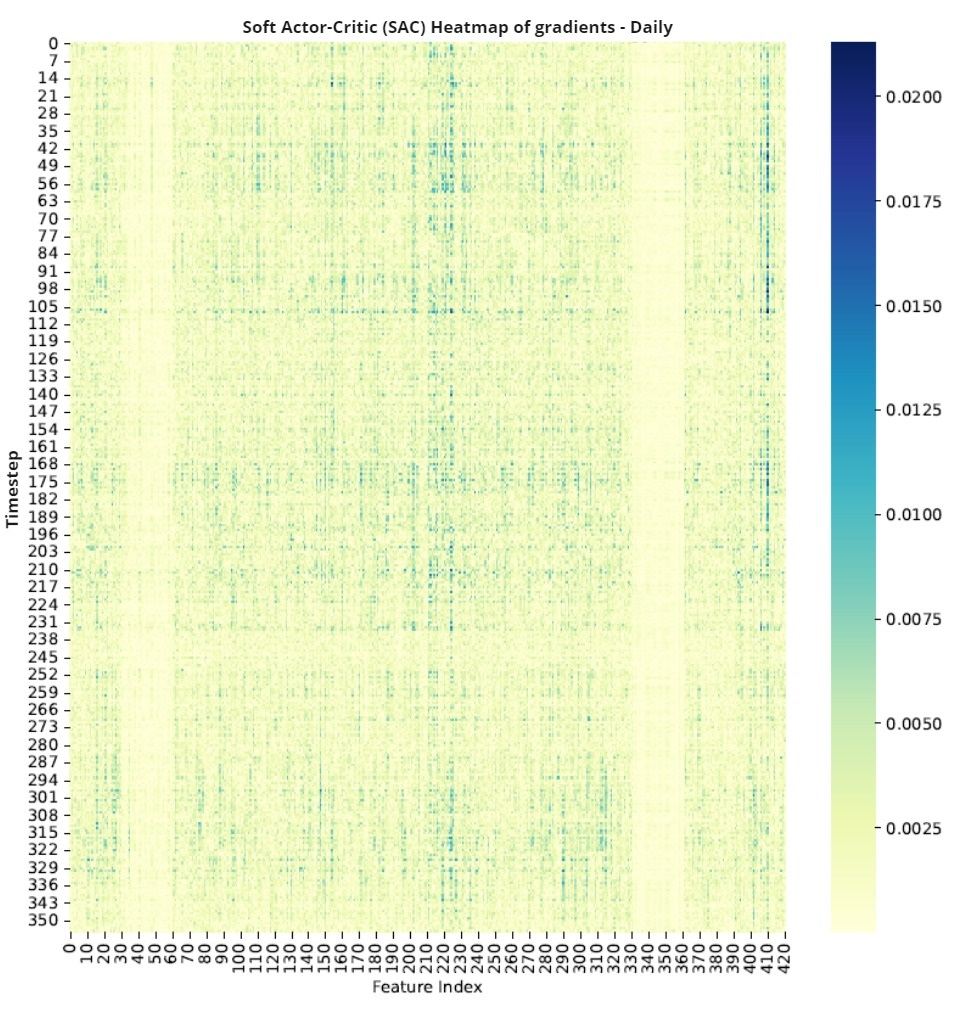
\includegraphics[width=0.8\textwidth]{figs/Heatmap_daily_SAC_random.jpg}
    \caption{Heatmap of gradients for the SAC model: The agent tends to ignore random features (330 - 360) as well as certain stocks, represented by features 30 - 60. The agent was trained on daily data without incorporating sentiment.}

    \label{fig:Heatmap_daily_SAC_random}
\end{figure}


In Figure \ref{fig:Heatmap_daily_PPO_importantdays}, we present the heatmap of gradients for the PPO model trained on daily data with sentiment incorporation. A striking observation from this heatmap is the presence of higher gradients on specific days, irrespective of the features. This indicates that the agent assigns more importance to these particular days, possibly due to significant market events or shifts in sentiment on those days.



\begin{figure}[h]
    \centering
    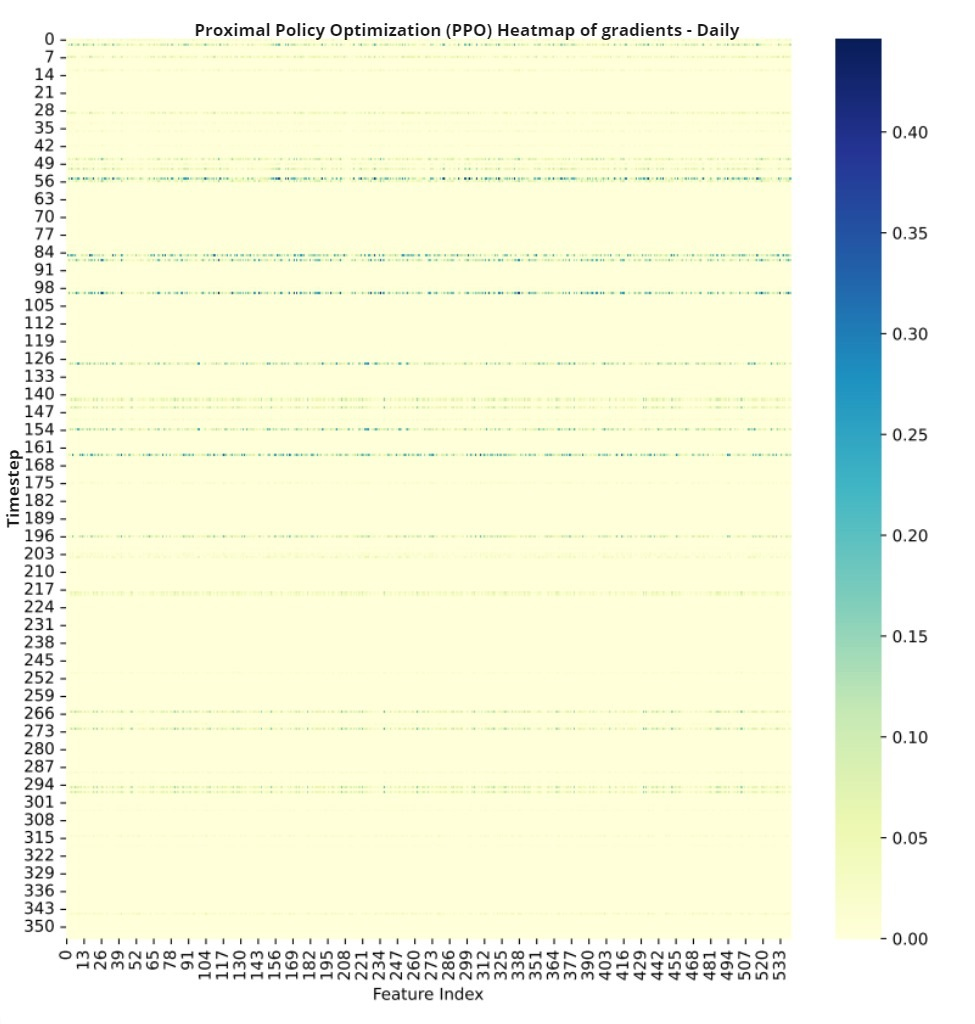
\includegraphics[width=0.8\textwidth]{figs/Heatmap_daily_PPO_importantdays.jpg}
    \caption{Heatmap of gradients for the PPO model: The agent has a higher gradient on some days, but not depending on features. The agent was trained on daily data incorporating sentiment.}

    \label{fig:Heatmap_daily_PPO_importantdays}
\end{figure}

Another interesting observation emerges from the heatmap of the SAC model trained on hourly data with sentiment incorporation, as shown in Figure \ref{Heatmap_hourly_SAC_featureImportance}. This heatmap distinctly showcases the agent's ability to prioritize certain features, as evidenced by the higher gradients. Such behavior indicates that the model has identified these features as particularly influential in its decision-making process.

However, it's worth noting that the agent does not exhibit any clear prioritization for specific days, suggesting that the temporal aspect might not be as influential for this model configuration. Additionally, the presence of gradients for random variables is a reminder that while the model can discern and prioritize meaningful features, it doesn't always disregard noise or irrelevant data entirely. This behavior underscores the importance of further refining the model or possibly introducing regularization techniques to minimize the influence of such noise.

\begin{figure}[h]
    \centering
    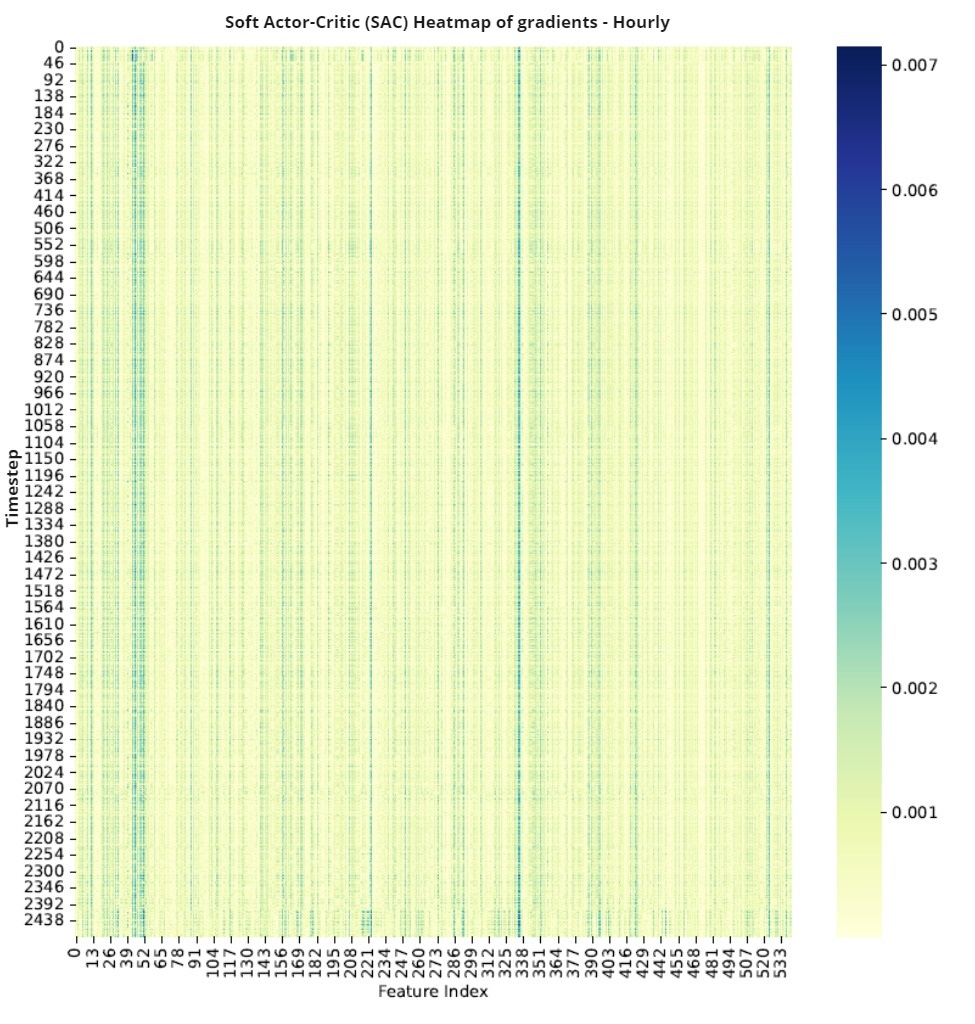
\includegraphics[width=0.8\textwidth]{figs/Heatmap_hourly_SAC_featureImportance.jpg}
    \caption{Heatmap of gradients for the SAC model trained on hourly data with sentiment: The agent exhibits clear feature prioritization, as indicated by higher gradients (features 40 - 52, 222, 337). However, there's no discernible prioritization for specific days, and gradients are also observed for random variables, suggesting the model's sensitivity to noise or irrelevant data.}
    \label{Heatmap_hourly_SAC_featureImportance}
\end{figure}


\subsubsection{Evaluating Temporal Effects on Predictions}

As observed in Figure \ref{fig:Heatmap_daily_PPO_importantdays}, certain agents demonstrate a distinct behavior where specific days hold more significance than others in their decision-making process. The PPO model, in particular, exhibits this tendency consistently for both daily and hourly data configurations. To delve deeper into this temporal effect, we computed the sum of gradients across all features for each date within the training range. The results of this computation are visualized in the subsequent figure.

\begin{figure}[h]
\centering
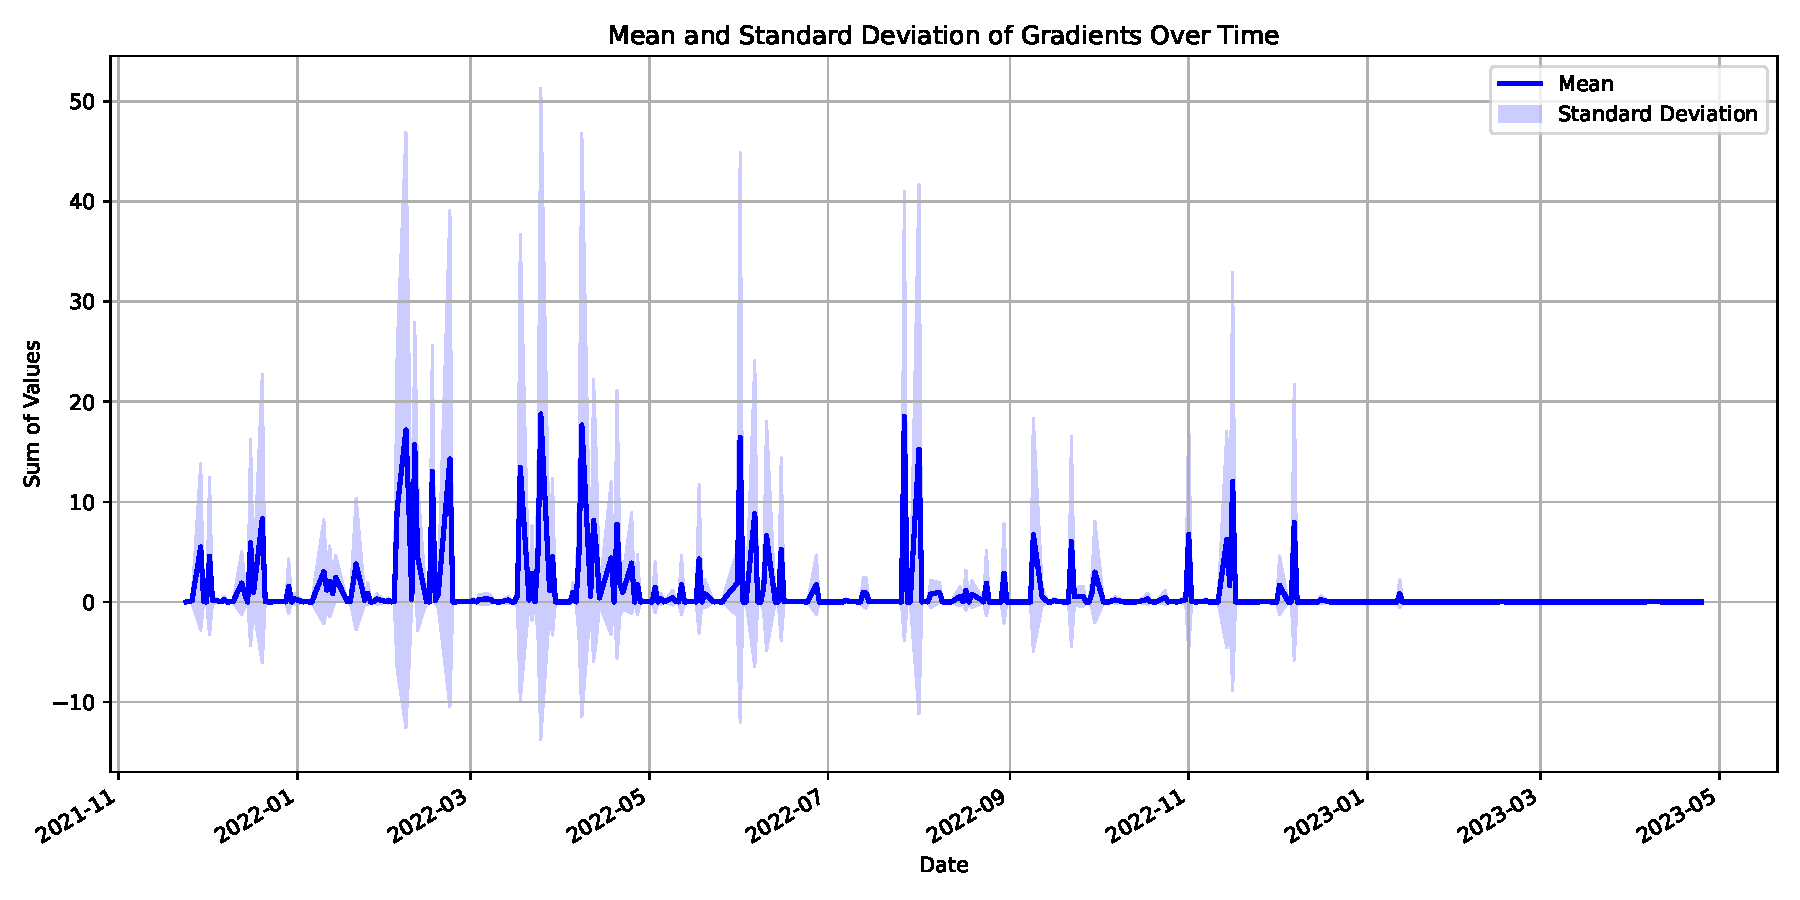
\includegraphics[width=1\textwidth]{figs/DayImportance_PPO_daily_NoSentiment.pdf}
\caption{Temporal Gradient Distribution for PPO Agent Trained on Daily Data Without Sentiment}
\label{fig:DayImportance_PPO_daily_NoSentiment}
\end{figure}

The visualization in Figure \ref{fig:DayImportance_PPO_daily_NoSentiment} presents the gradients over time for the PPO agent trained on daily data without sentiment. A striking observation is the pronounced spike in gradients at the beginning of 2022. This heightened sensitivity correlates with the onset of the military conflict in Ukraine, which had substantial repercussions on global stock markets. Such events often lead to increased market volatility, with stocks reacting sharply to news and geopolitical developments. The PPO agent's heightened gradient during this period indicates its increased sensitivity and adaptability to these market shifts, emphasizing the importance of certain days or events in its decision-making process. This behavior underscores the capability of RL models like PPO to dynamically adjust their strategies in response to significant market events, even when not explicitly trained on sentiment data.

\begin{figure}[h]
\centering
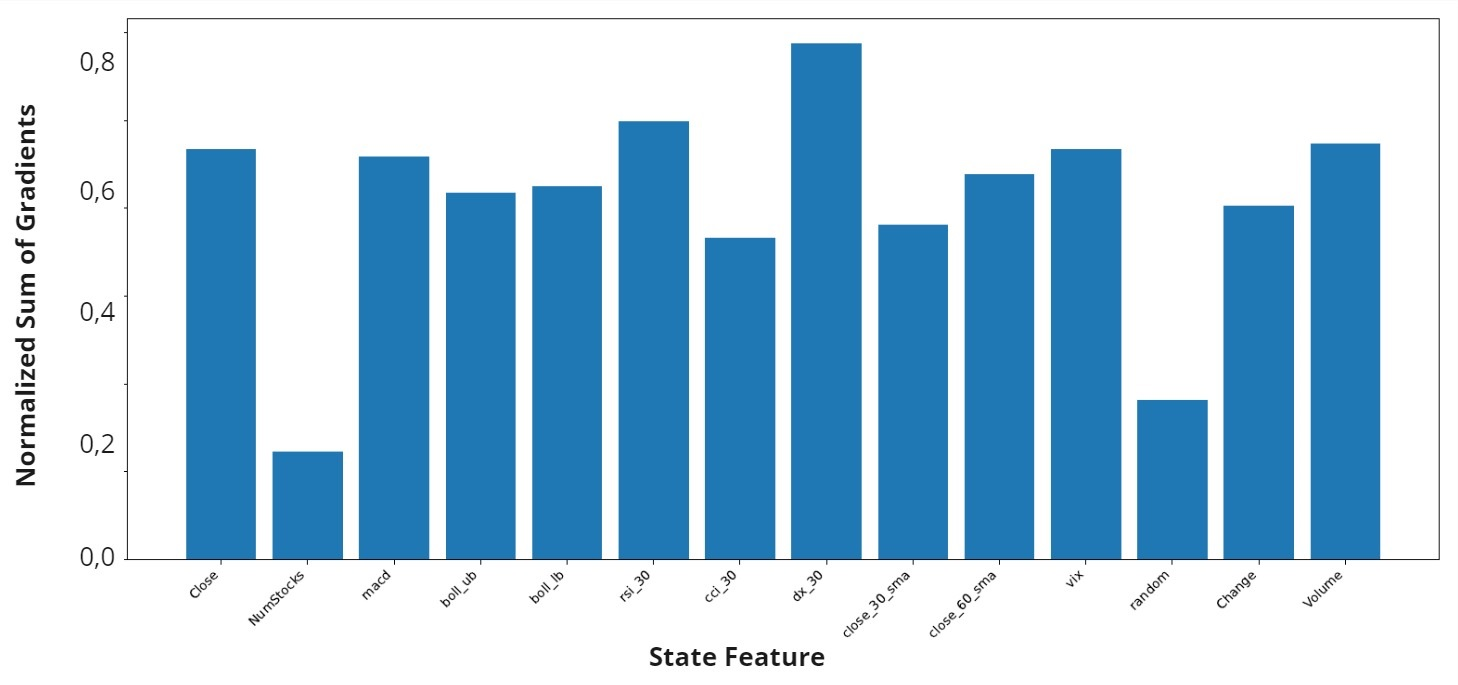
\includegraphics[width=1\textwidth]{figs/FeatureImportance_SAC_daily.jpg}
\caption{Feature Importance Visualization for SAC Agent on Daily Data without Sentiment: Emphasis on the `dx 30` Technical Indicator and Disregard of Random Variables}
\label{fig:FeatureImportance_SAC_daily}
\end{figure}

\begin{figure}[h]
\centering
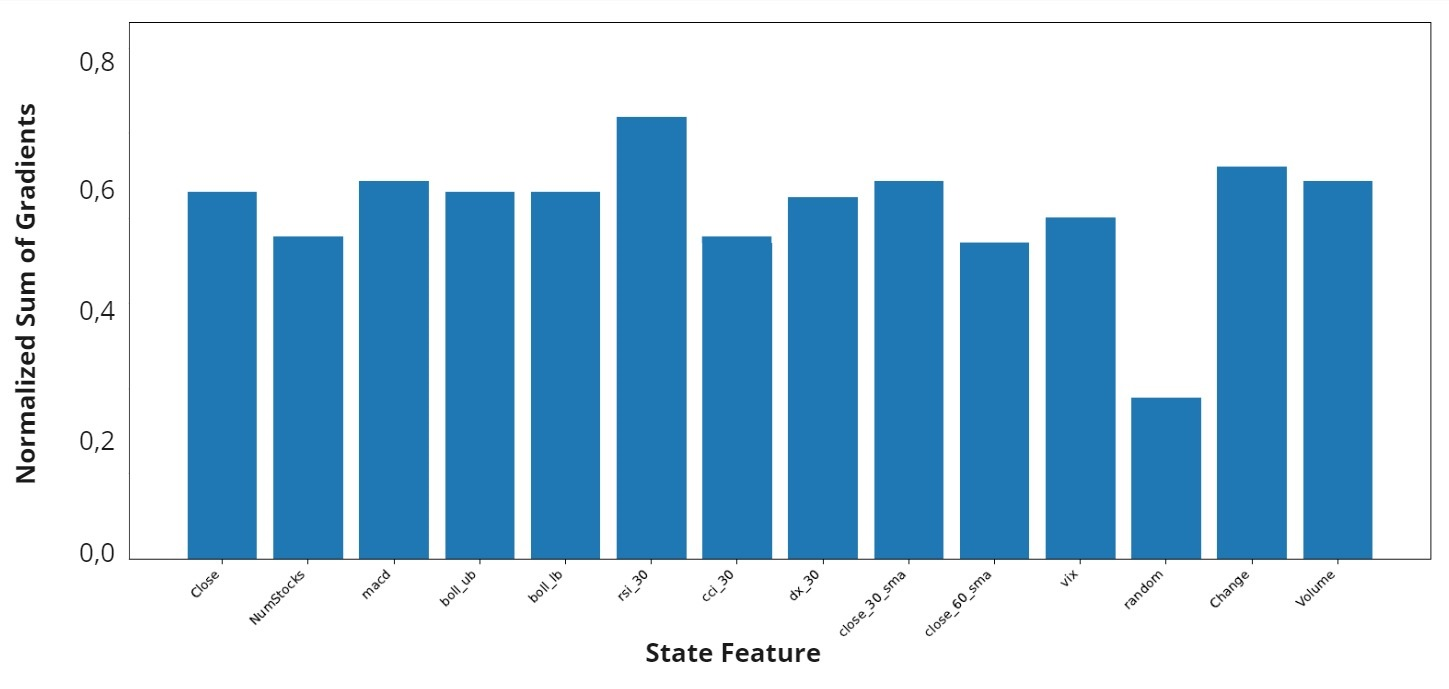
\includegraphics[width=1\textwidth]{figs/FeatureImportance_SAC_hourly.jpg}
\caption{Feature Importance Visualization for SAC Agent on Hourly Data without Sentiment: Subtle Emphasis on the `dx 30` Technical Indicator and Disregard for Random Variables}
\label{fig:FeatureImportance_SAC_hourly}
\end{figure}

Figures \ref{fig:FeatureImportance_SAC_daily} and \ref{fig:FeatureImportance_SAC_hourly} provide a visual representation of feature importance for the SAC agent trained on daily and hourly data, respectively, without sentiment.

From the plots, it's evident that the agent effectively disregards the random variable, as indicated by its low gradient. This behavior is consistent with our earlier observations from the heatmap, underscoring the model's ability to filter out noise or irrelevant data. Additionally, the agent seems to downplay the significance of certain stocks, suggesting that not all stocks contribute equally to its decision-making process.

Among the features, the technical indicator dx 30 stands out with a noticeably higher gradient, especially in the daily data plot. This indicates that the SAC agent attributes a higher importance to this particular technical indicator compared to others. While this distinction is more pronounced in the daily data, a similar trend, albeit less distinct, is observable in the hourly data plot. The elevated gradient for dx 30 suggests that this technical indicator might be a more influential factor in the agent's decision-making process, potentially due to its ability to capture specific market dynamics or trends.

These observations emphasize the nuanced behavior of the SAC agent, highlighting its capability to discern and prioritize specific features while filtering out less relevant information. Such insights are invaluable for refining the model further and tailoring its training to emphasize key indicators.

\begin{figure}[h]
\centering
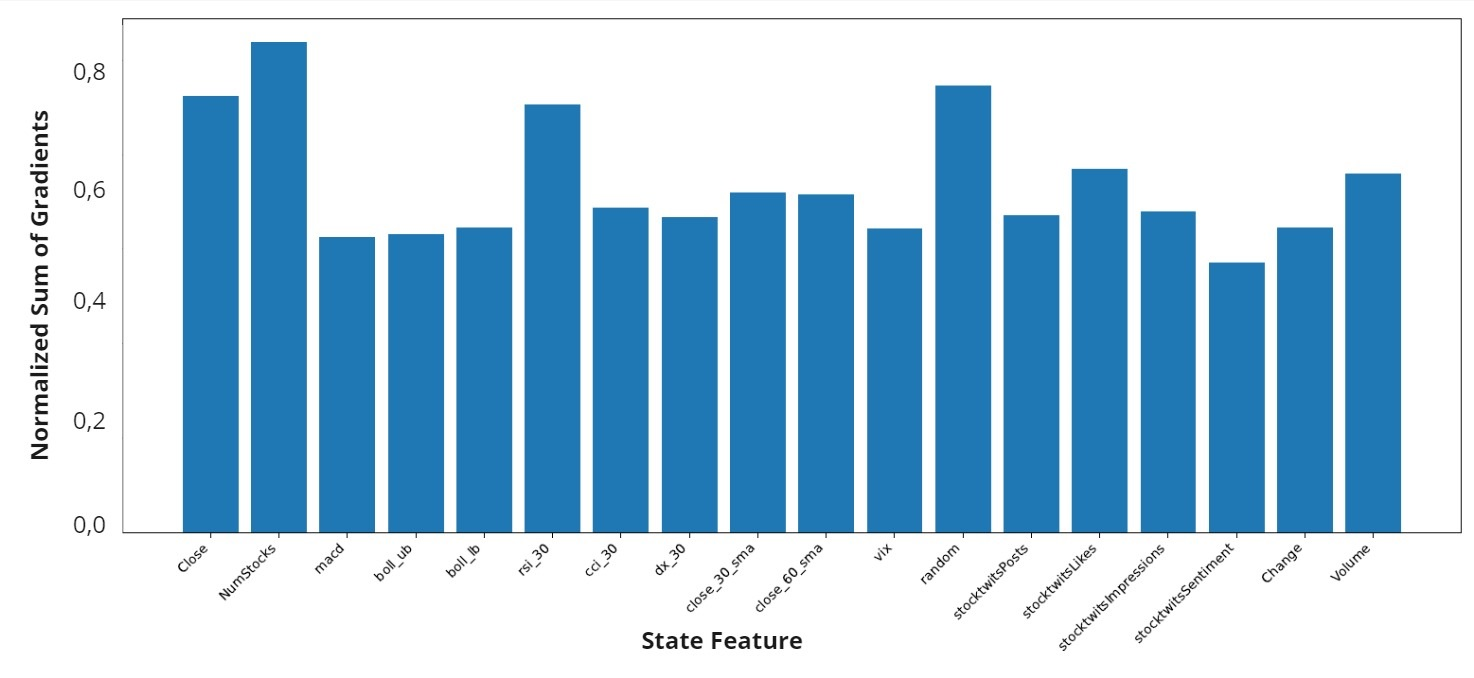
\includegraphics[width=1\textwidth]{figs/FeatureImportance_Sentiment_SAC_daily.jpg}
\caption{Feature Importance Visualization for SAC Agent on Daily Data with Sentiment: A relatively uniform gradient distribution with notable peaks for the number of stocks, random variables, and the `dx 30` technical indicator.}
\label{fig:FeatureImportance_Sentiment_SAC_daily}
\end{figure}


The figure \ref{fig:FeatureImportance_Sentiment_SAC_daily} provides an intriguing perspective on the SAC agent's behavior when trained on daily data with sentiment. While most features exhibit a relatively uniform gradient, suggesting a balanced consideration by the agent, there are distinct peaks for the number of stocks, random variables, and notably, the dx 30 technical indicator.

The prominence of random variables in the gradient distribution is particularly interesting. Given the extensive state length of 541, it's plausible that the agent is overwhelmed with information, leading to a diffusion of feature importance. This "information saturation" might cause the agent to inadvertently assign significance to even the random numbers, mistaking noise for potentially valuable data. Such behavior underscores the challenges of training models on high-dimensional data and emphasizes the need for effective feature selection and engineering to guide the agent towards more meaningful patterns.

\subsubsection{Assessing the Impact of Individual Stocks}
\begin{figure}[h]
\centering
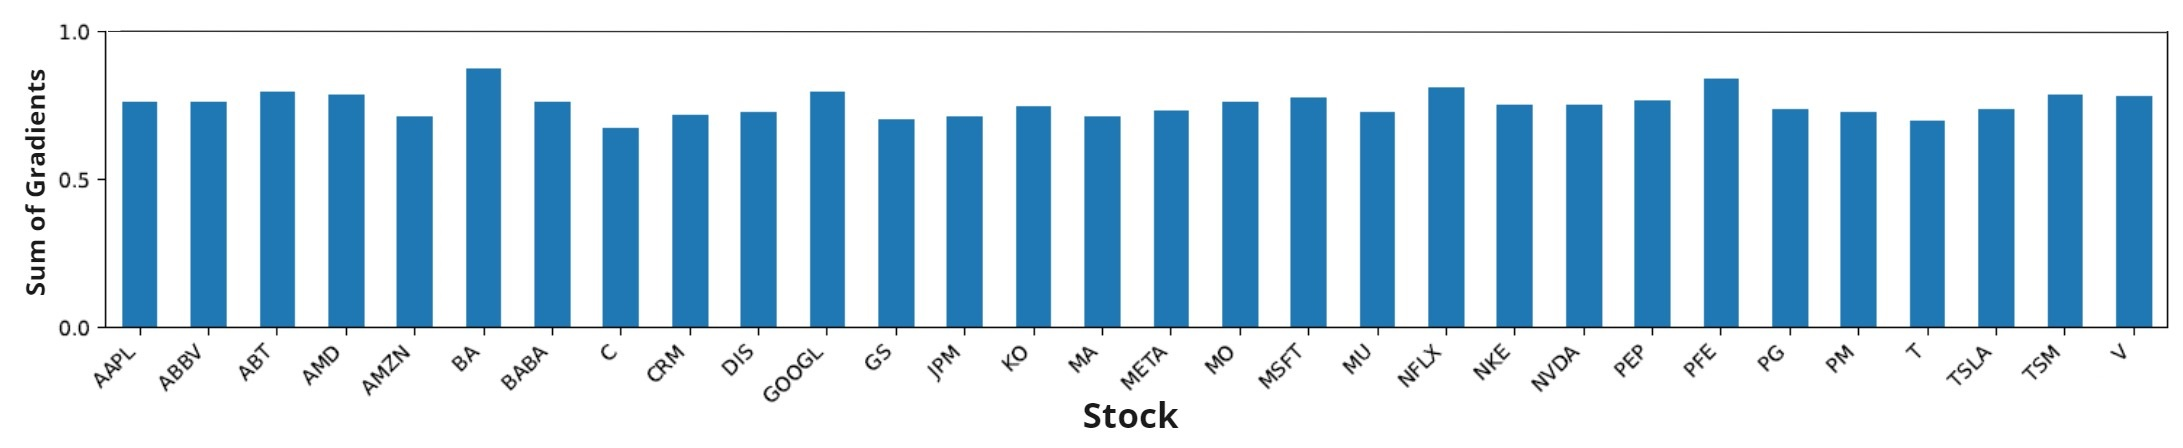
\includegraphics[width=1\textwidth]{figs/Stock_Importance_SAC_daily.jpg}
\caption{Stock Importance Visualization for SAC Agent on Daily Data without Sentiment: Consistent Gradient Distribution Across Different Stocks.}
\label{fig:StockImportance_SAC_daily}
\end{figure}

The Figure \ref{fig:StockImportance_SAC_daily} offers a perspective on the stock-specific importance as perceived by the SAC agent when trained on daily data without sentiment. Interestingly, the gradient sums for individual stocks appear to be uniformly distributed. This suggests that the agent does not exhibit a strong preference or bias towards any particular stock, treating them with relatively equal importance. While this uniformity ensures a balanced consideration of stocks, it also raises questions about the agent's ability to discern nuanced patterns or trends specific to individual stocks.

\section{Discussion and Future Work} 
\label{sec:disccution}
In summary the reinforcement learning approach for stock trading was very successful. Even the proven method of buy and hold and portfolio theory could be outperformed while remaining in the same risk thresholds regarding the calmar ratio and sharp ratio. Additionally, the developed pipeline from data collection, pre-processing and feature engineering to model training and holistic backtesting can be applied on all various alternative data sets. As the state of our model was already very large, the other data sets had to be omitted. But this approach -- as it looks very promising -- should be replicated with fundamental data, senate trading or other alternative data. Due to the explainability of sensitivity analysis the risk exposure can be reduced additionally since obvious randomly acting agents can be rejected. Nonetheless, our approach was expected to give the opportunity to reduce the dimensions of our state. However, since the sensitivity analysis could not exclude single features with significant confidence, the models could not be re-trained and benchmarked with a reduced state. Similarly our efforts in terms of model parameter optimisation resulted in stagnating improvements. The most likely reason is the low signal-to-noise ratio. To overcome this obstacle, one should focus even stronger on data cleaning and feature engineering. While the Kalmar filter showed significant improvements, one could follow completely different data representation: instead of time bars, one could adapt volume or tick bars and other novel approaches to produce stable signals from noisy data. However, these strategies are all  outside of reinforcement learning and therefore not relevant for this thesis.


\bibliographystyle{plain}
\bibliography{references}  %%% Uncomment this line and comment out the ``thebibliography'' section below to use the external .bib file (using bibtex) .


%%% Uncomment this section and comment out the \bibliography{references} line above to use inline references.
% \begin{thebibliography}{1}

% 	\bibitem{kour2014real}
% 	George Kour and Raid Saabne.
% 	\newblock Real-time segmentation of on-line handwritten arabic script.
% 	\newblock In {\em Frontiers in Handwriting Recognition (ICFHR), 2014 14th
% 			International Conference on}, pages 417--422. IEEE, 2014.

% 	\bibitem{kour2014fast}
% 	George Kour and Raid Saabne.
% 	\newblock Fast classification of handwritten on-line arabic characters.
% 	\newblock In {\em Soft Computing and Pattern Recognition (SoCPaR), 2014 6th
% 			International Conference of}, pages 312--318. IEEE, 2014.

% 	\bibitem{hadash2018estimate}
% 	Guy Hadash, Einat Kermany, Boaz Carmeli, Ofer Lavi, George Kour, and Alon
% 	Jacovi.
% 	\newblock Estimate and replace: A novel approach to integrating deep neural
% 	networks with existing applications.
% 	\newblock {\em arXiv preprint arXiv:1804.09028}, 2018.

% \end{thebibliography}



\appendix
\section{Pairwise Comparision - Daily}

\begin{figure}[h]
\centering
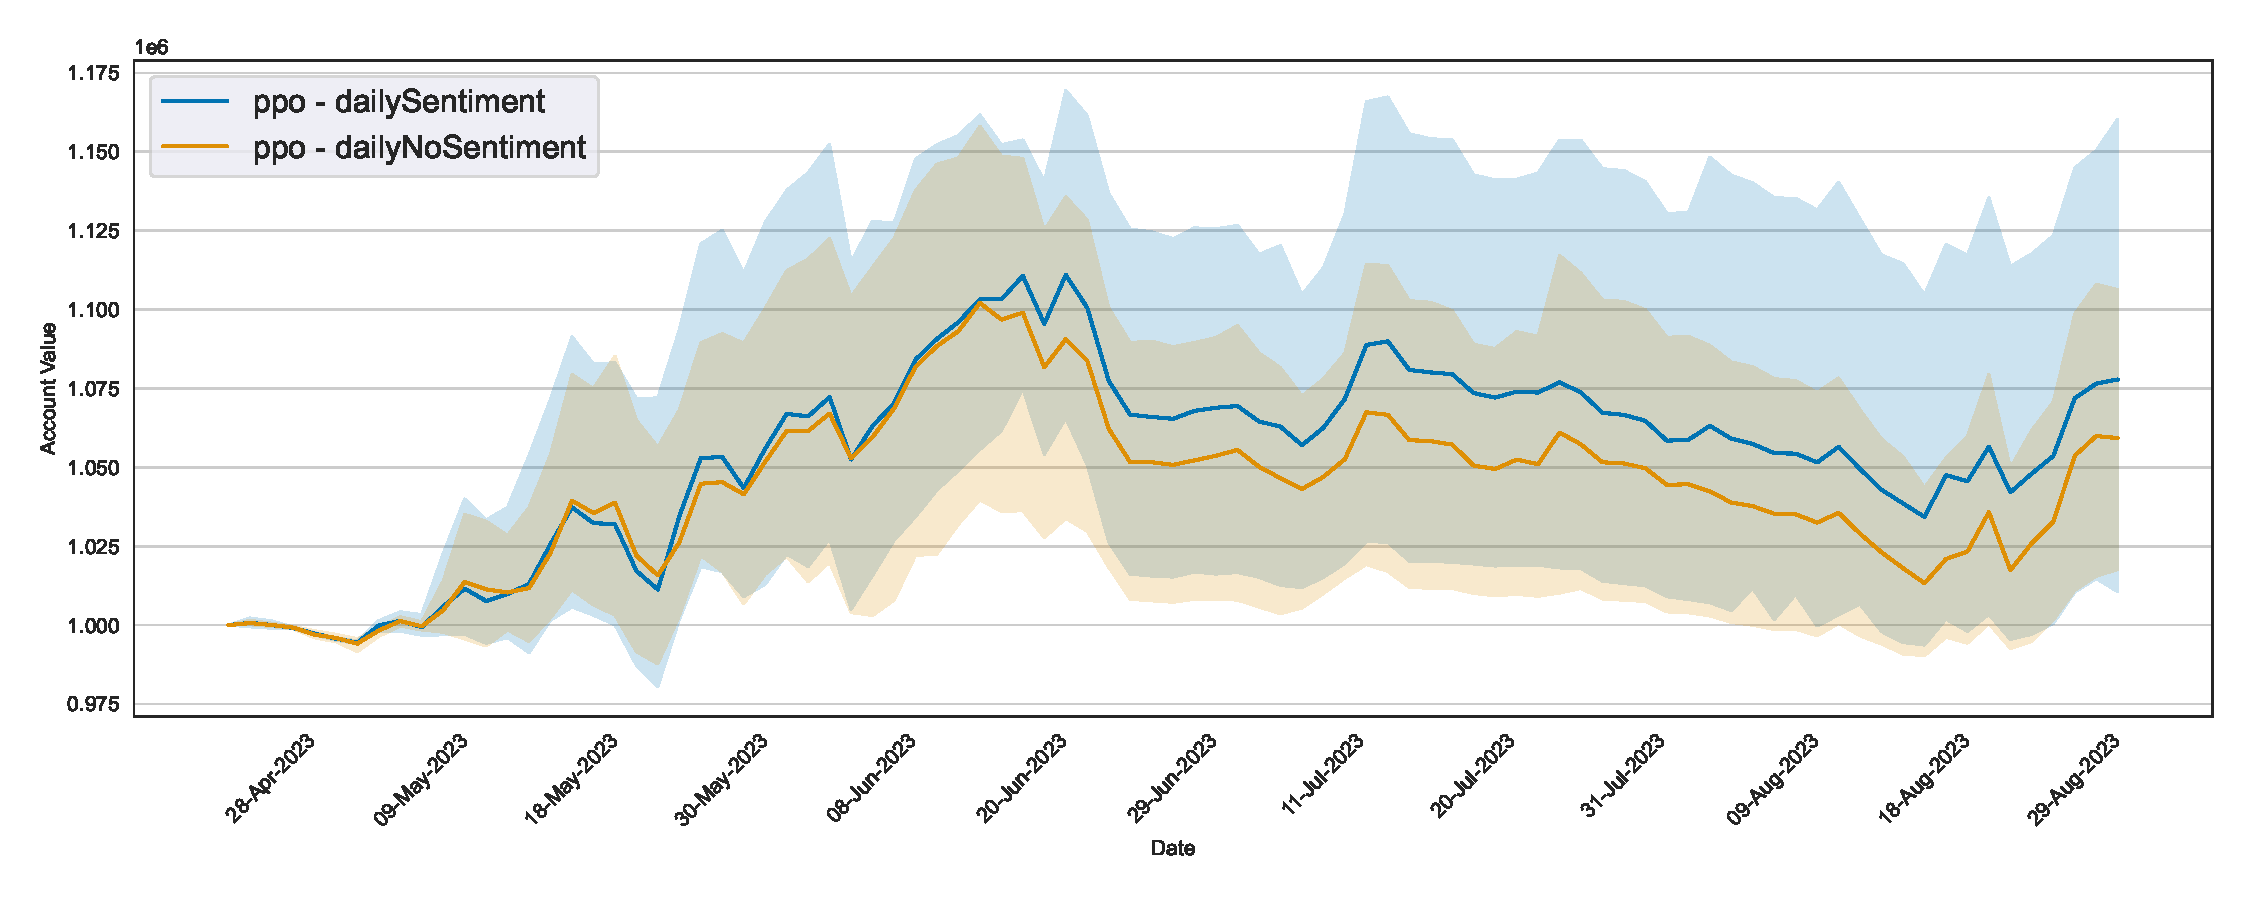
\includegraphics[width=1\textwidth]{figs/Models_comparison/Sentiment/Compare_agent_performance_dailySentiment_ppo.pdf}
\caption{Performance comparison of PPO agent trained on daily data with and without sentiment integration.}
\label{fig:Compare_agent_performance_dailySentiment_ppo}
\end{figure}

\begin{figure}[h]
\centering
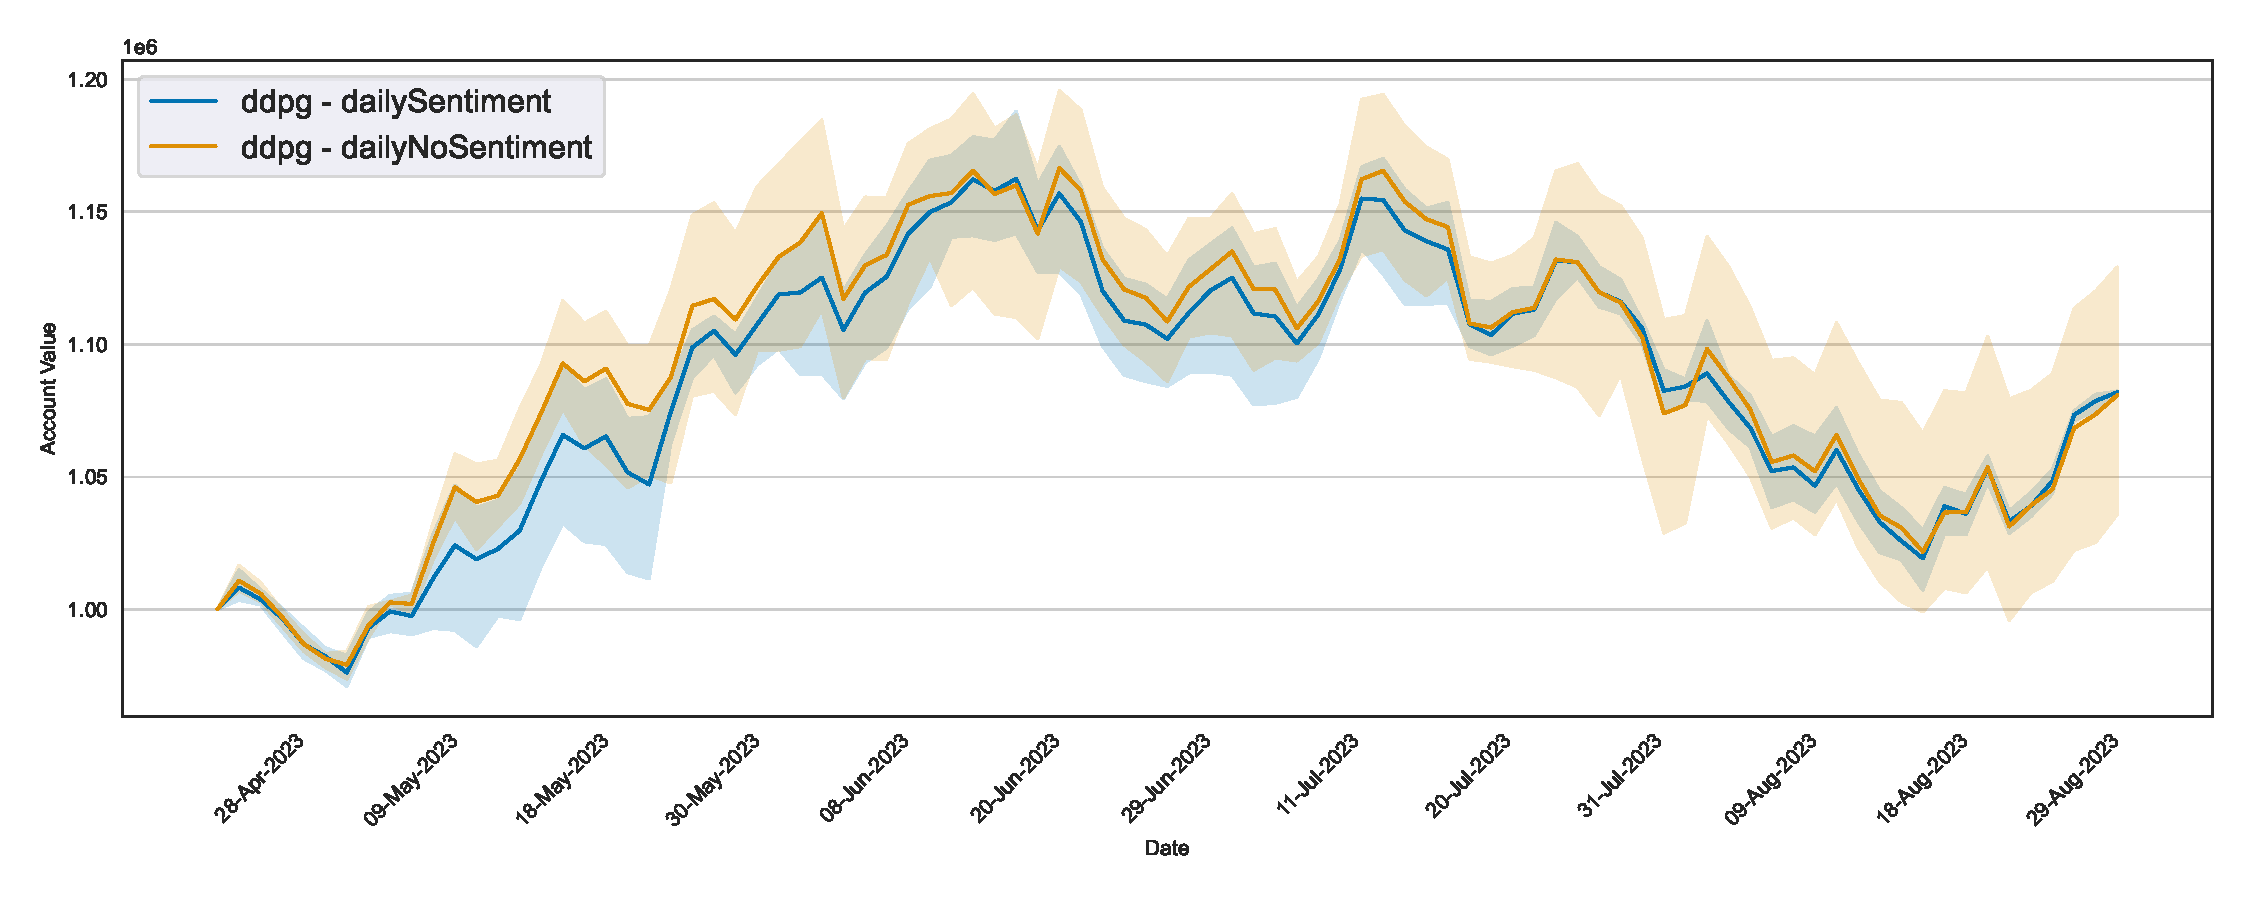
\includegraphics[width=1\textwidth]{figs/Models_comparison/Sentiment/Compare_agent_performance_dailySentiment_ddpg.pdf}
\caption{Performance comparison of DDPG agent trained on daily data with and without sentiment integration.}
\label{fig:Compare_agent_performance_dailySentiment_ddpg}
\end{figure}

\begin{figure}[h]
\centering
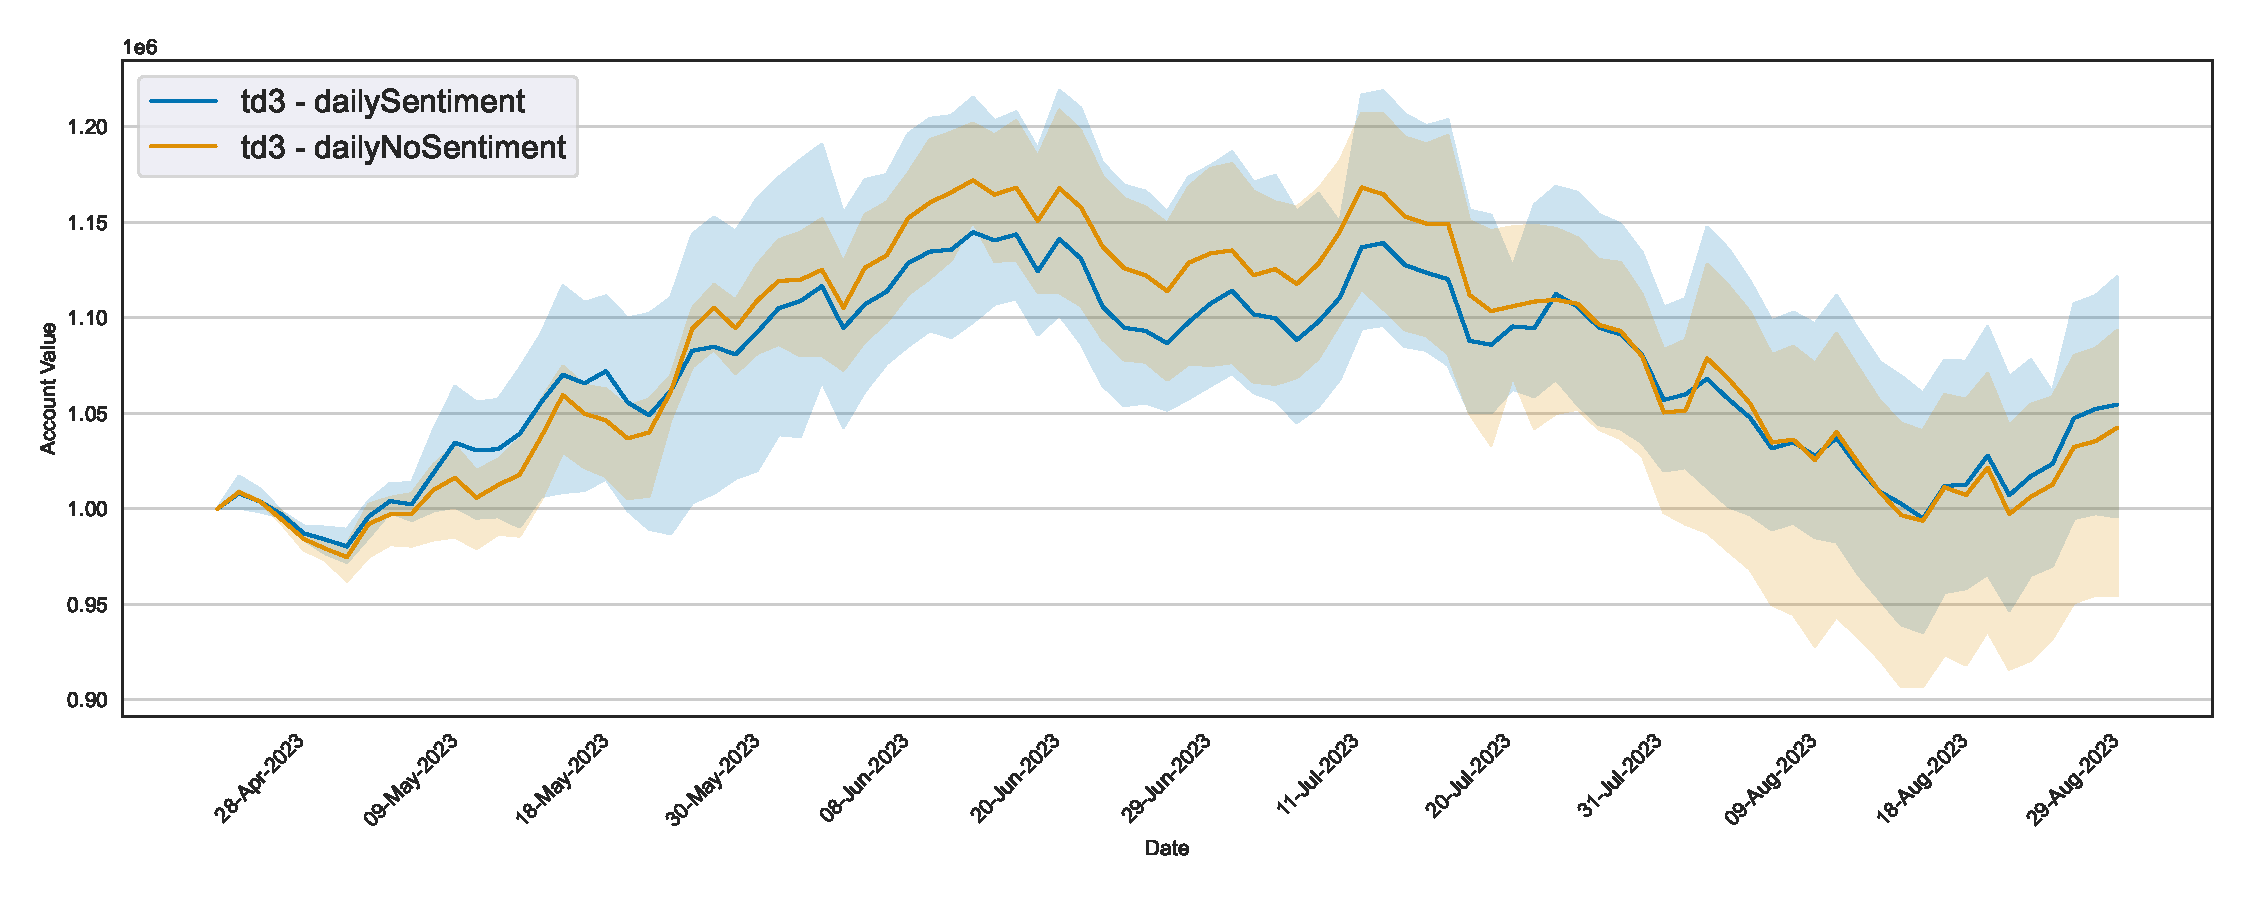
\includegraphics[width=1\textwidth]{figs/Models_comparison/Sentiment/Compare_agent_performance_dailySentiment_td3.pdf}
\caption{Performance comparison of TD3 agent trained on daily data with and without sentiment integration.}
\label{fig:Compare_agent_performance_dailySentiment_td3}
\end{figure}

\begin{figure}[h]
\centering
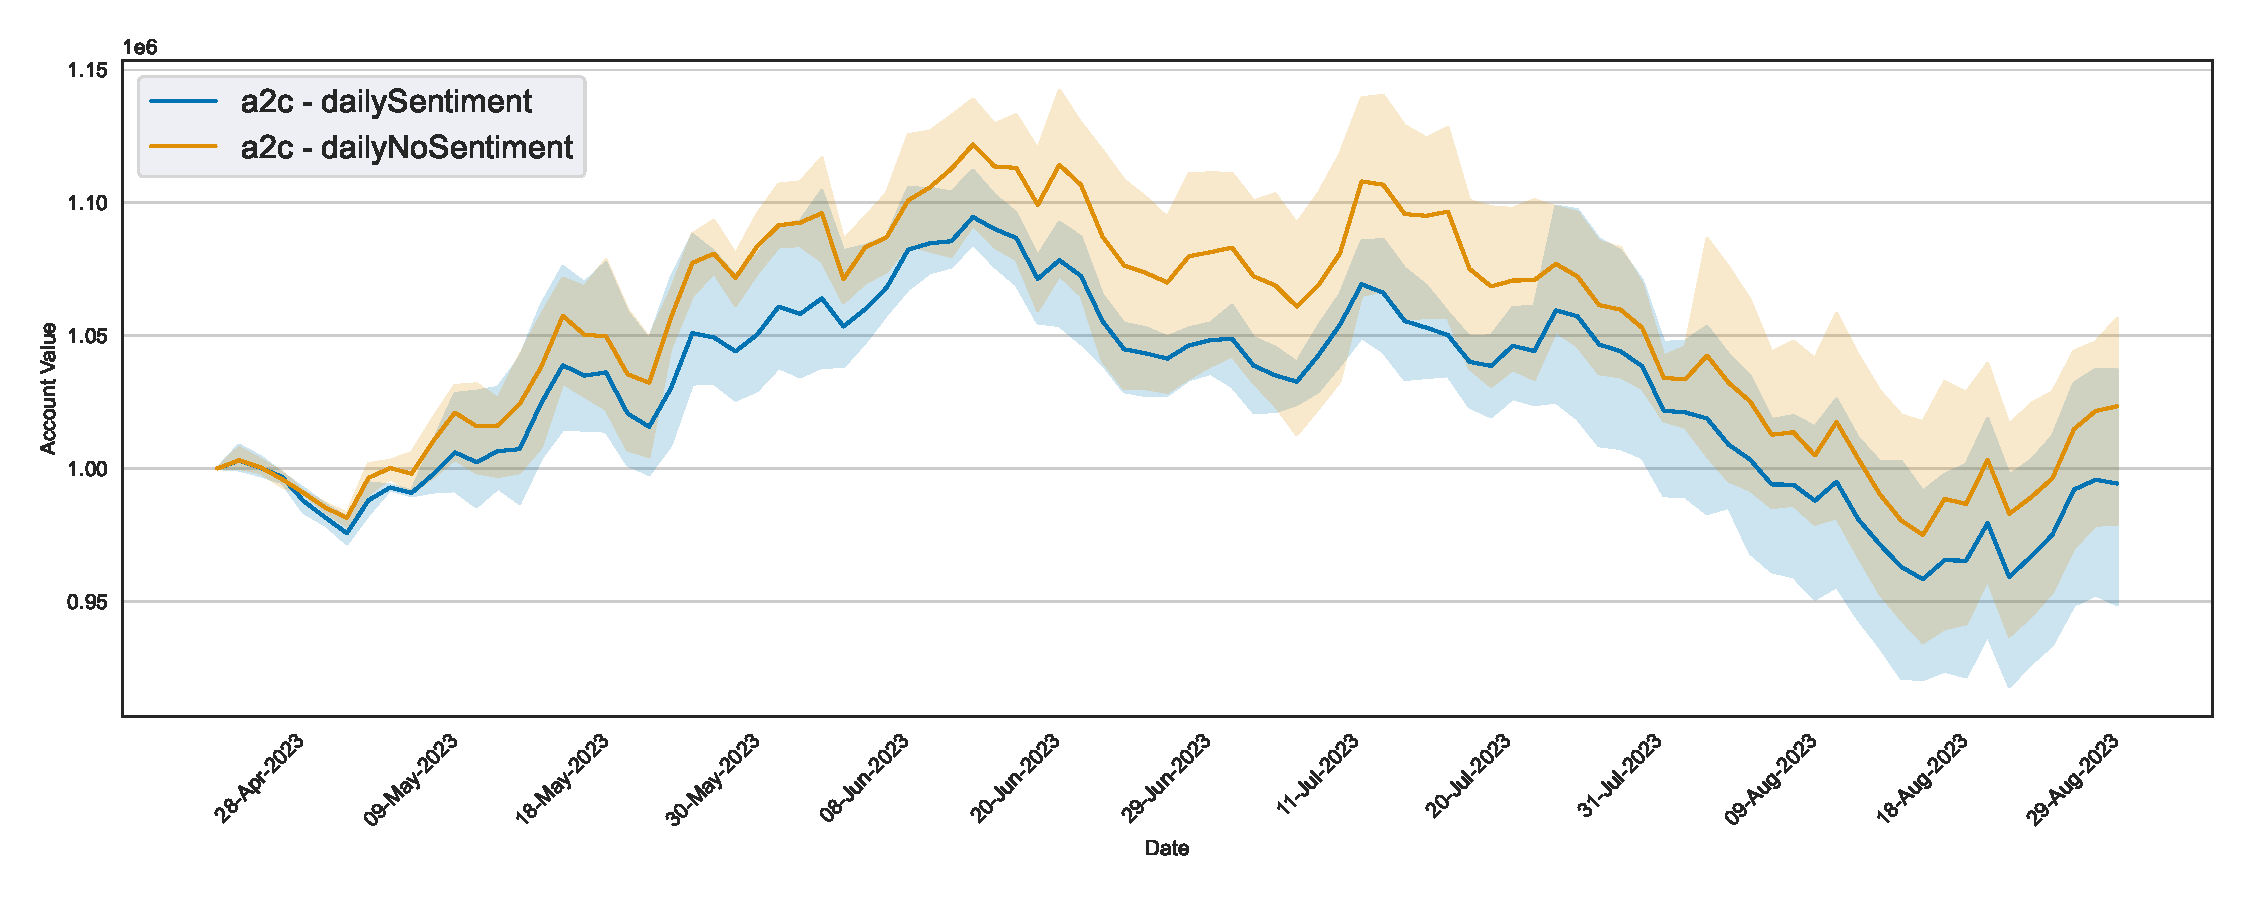
\includegraphics[width=1\textwidth]{figs/Models_comparison/Sentiment/Compare_agent_performance_dailySentiment_a2c.pdf}
\caption{Performance comparison of A2C agent trained on daily data with and without sentiment integration.}
\label{fig:Compare_agent_performance_dailySentiment_a2c}
\end{figure}

\begin{figure}[h]
\centering
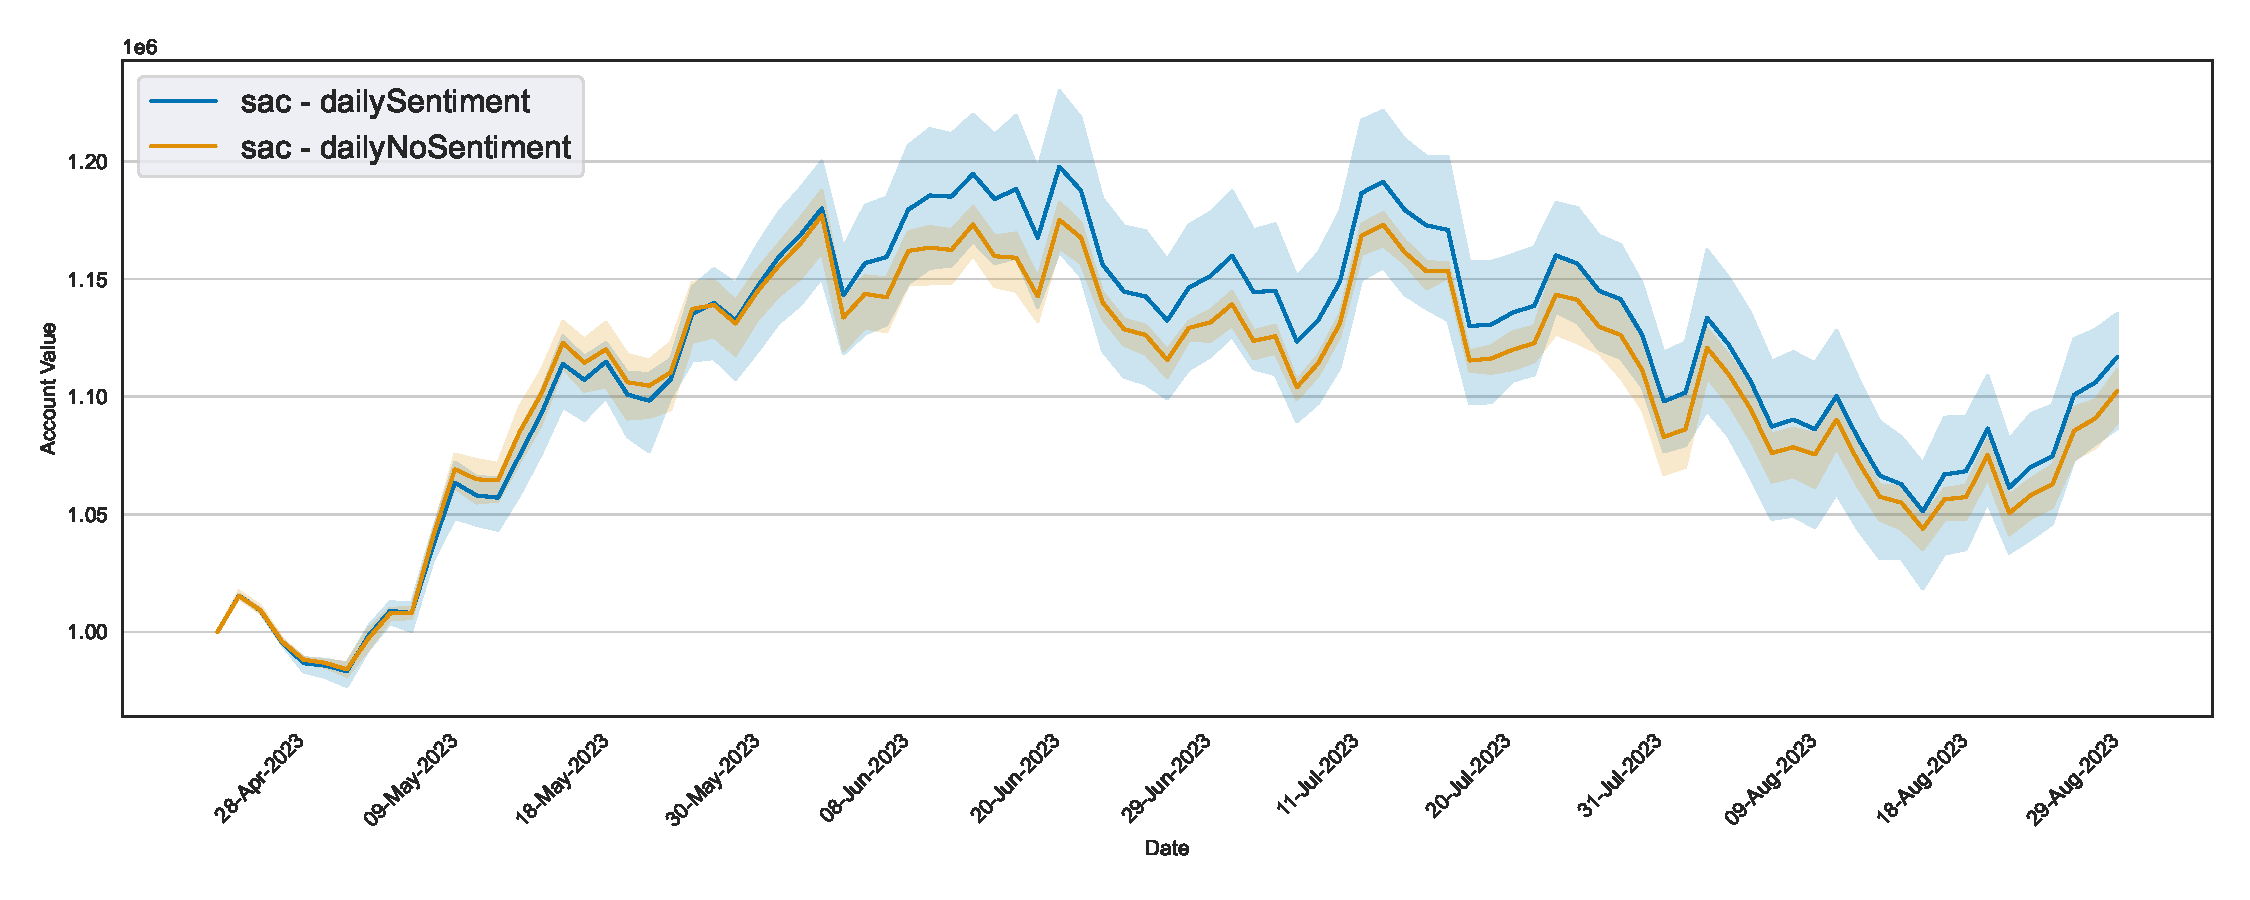
\includegraphics[width=1\textwidth]{figs/Models_comparison/Sentiment/Compare_agent_performance_dailySentiment_sac.pdf}
\caption{Performance comparison of SAC agent trained on daily data with and without sentiment integration.}
\label{fig:Compare_agent_performance_dailySentiment_sac}
\end{figure}


\section{Pairwise Comparision - Hourly}

\begin{figure}[h]
\centering
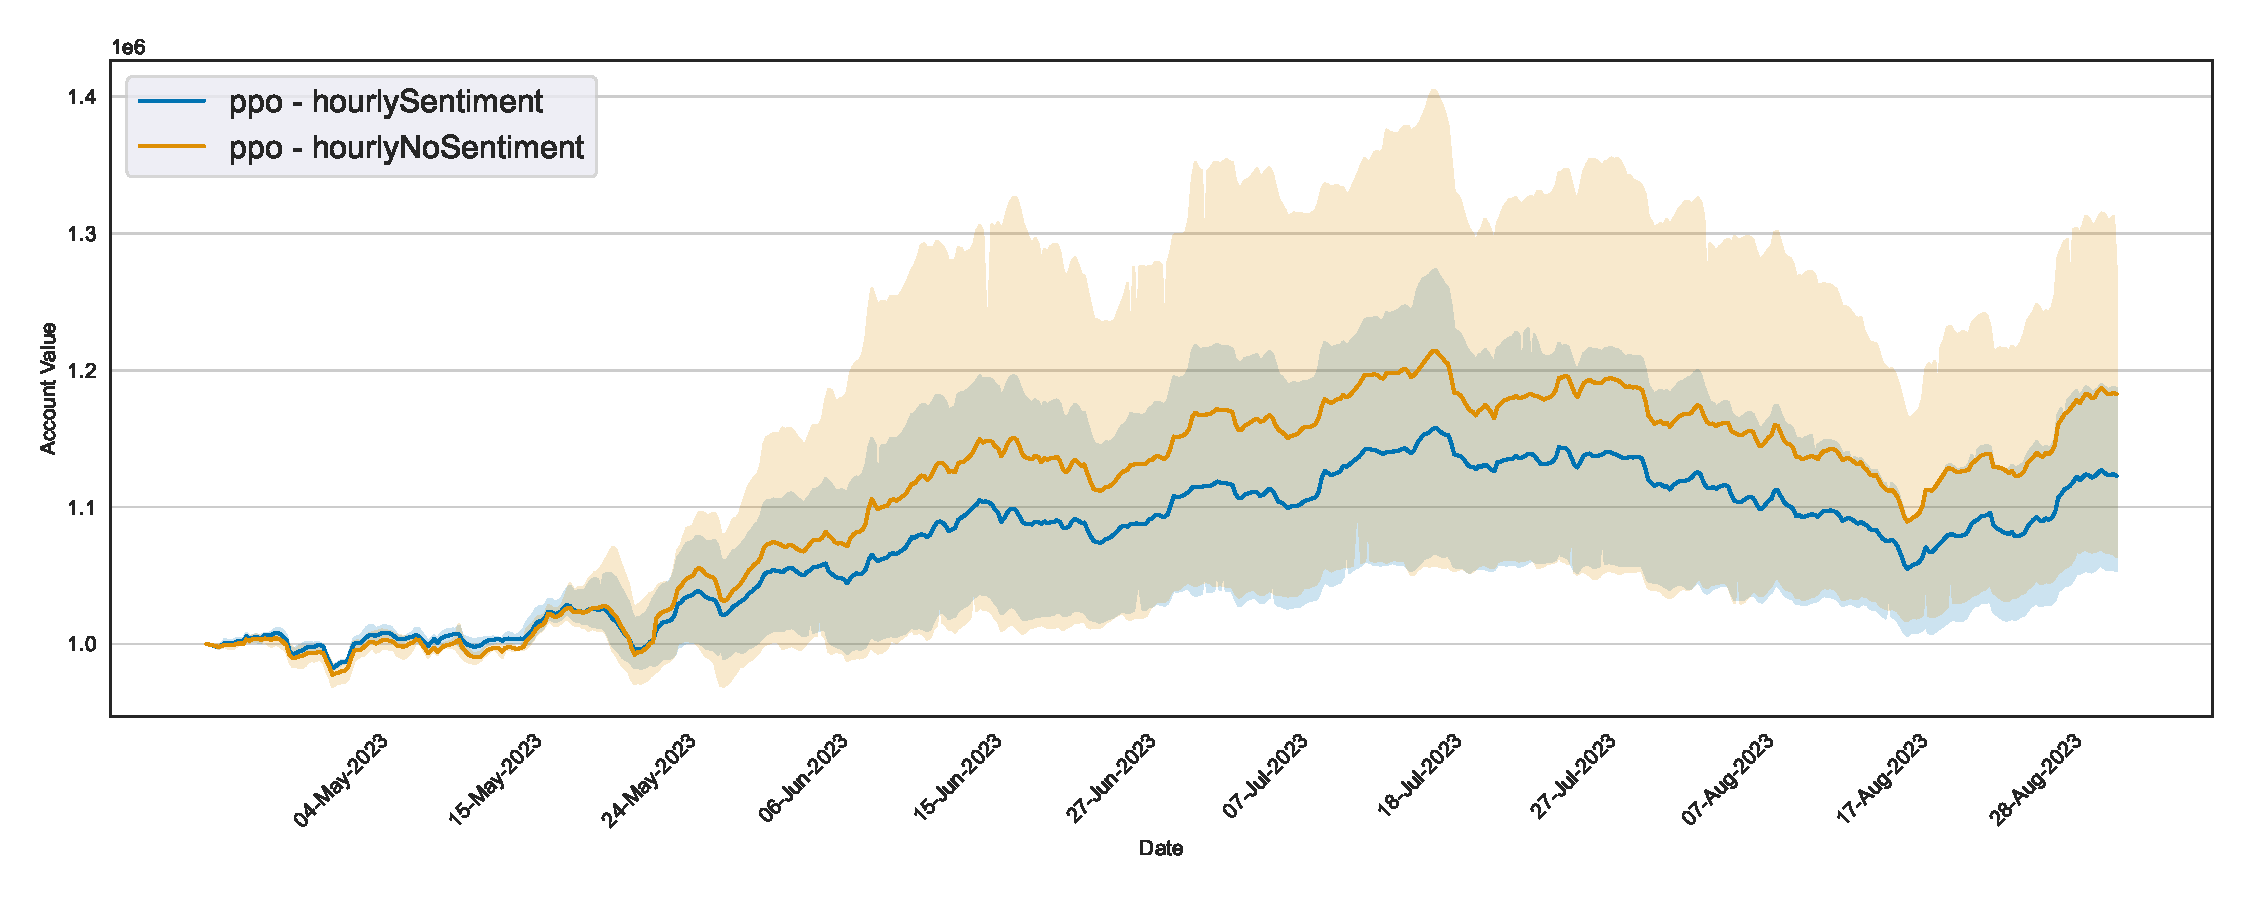
\includegraphics[width=1\textwidth]{figs/Models_comparison/Sentiment/Compare_agent_performance_hourlySentiment_ppo.pdf}
\caption{Performance comparison of PPO agent trained on hourly data with and without sentiment integration.}
\label{fig:Compare_agent_performance_hourlySentiment_ppo}
\end{figure}

\begin{figure}[h]
\centering
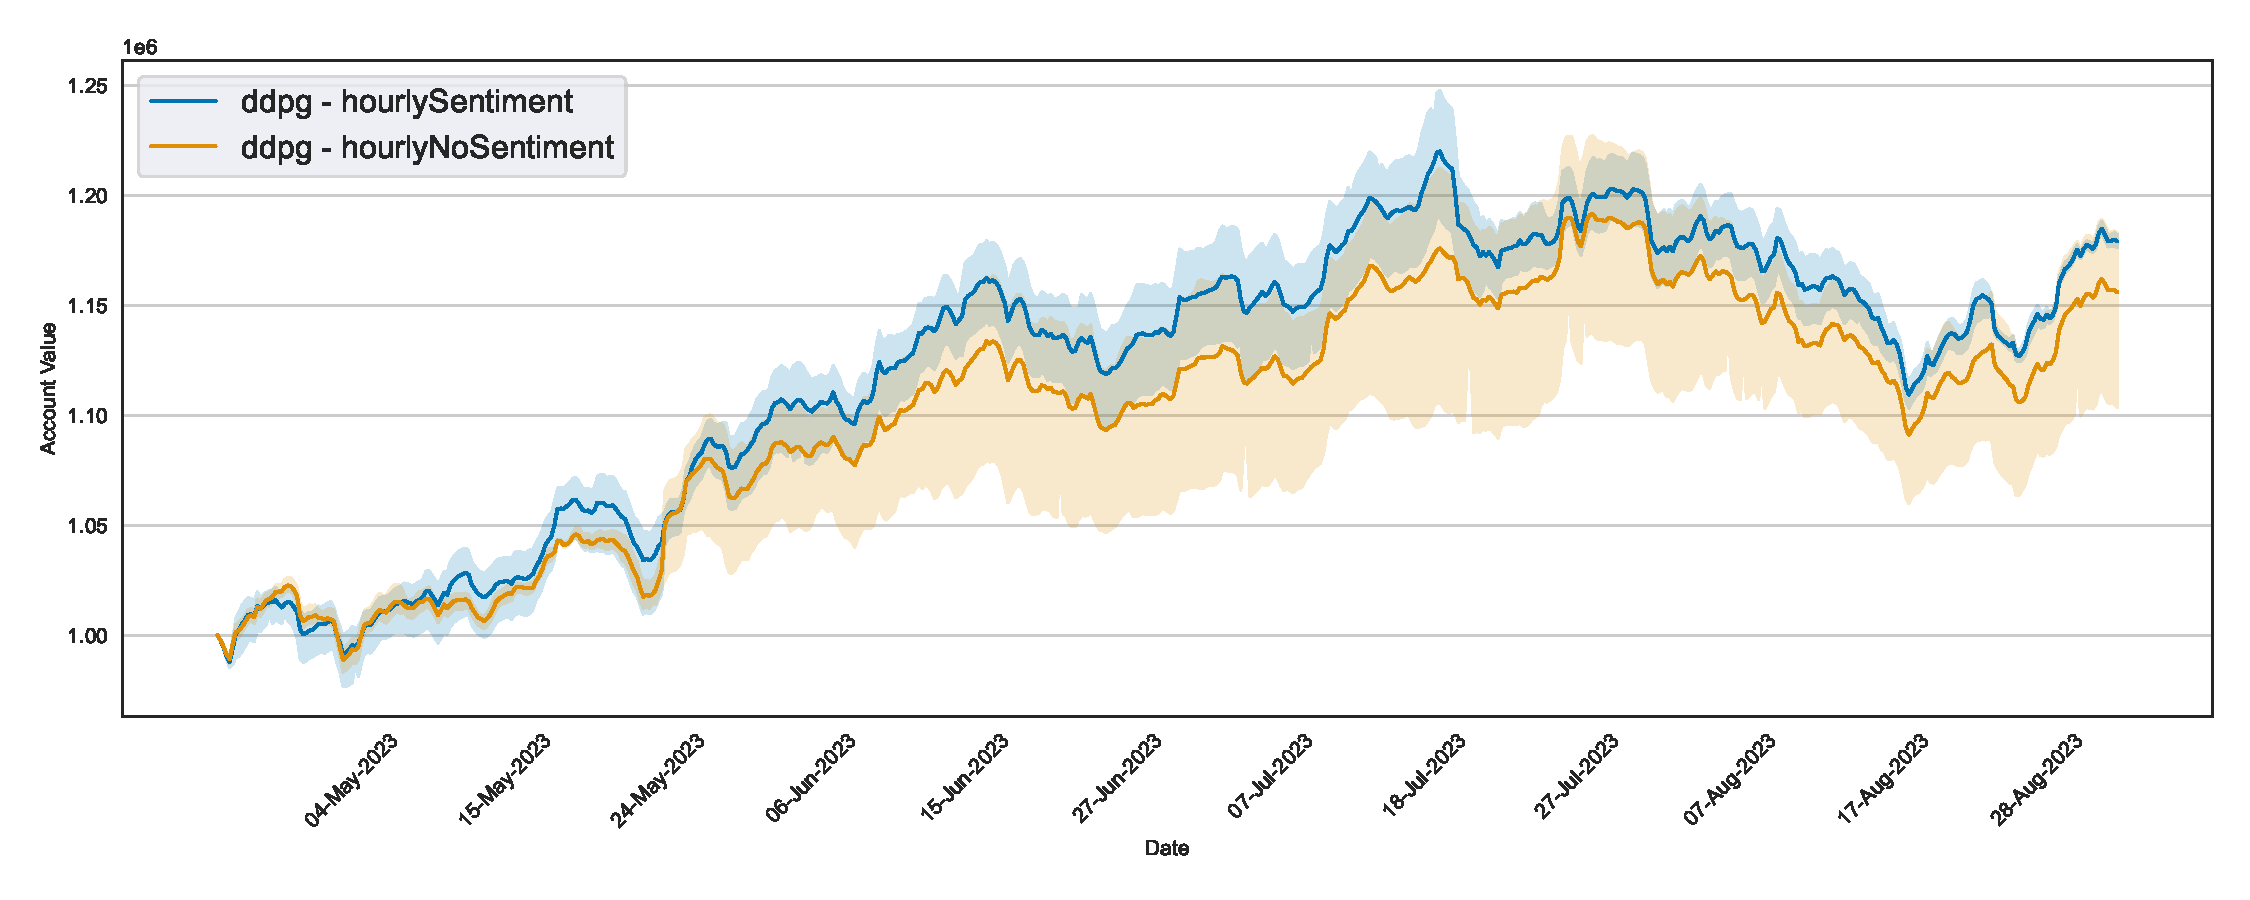
\includegraphics[width=1\textwidth]{figs/Models_comparison/Sentiment/Compare_agent_performance_hourlySentiment_ddpg.pdf}
\caption{Performance comparison of DDPG agent trained on hourly data with and without sentiment integration.}
\label{fig:Compare_agent_performance_hourlySentiment_ddpg}
\end{figure}

\begin{figure}[h]
\centering
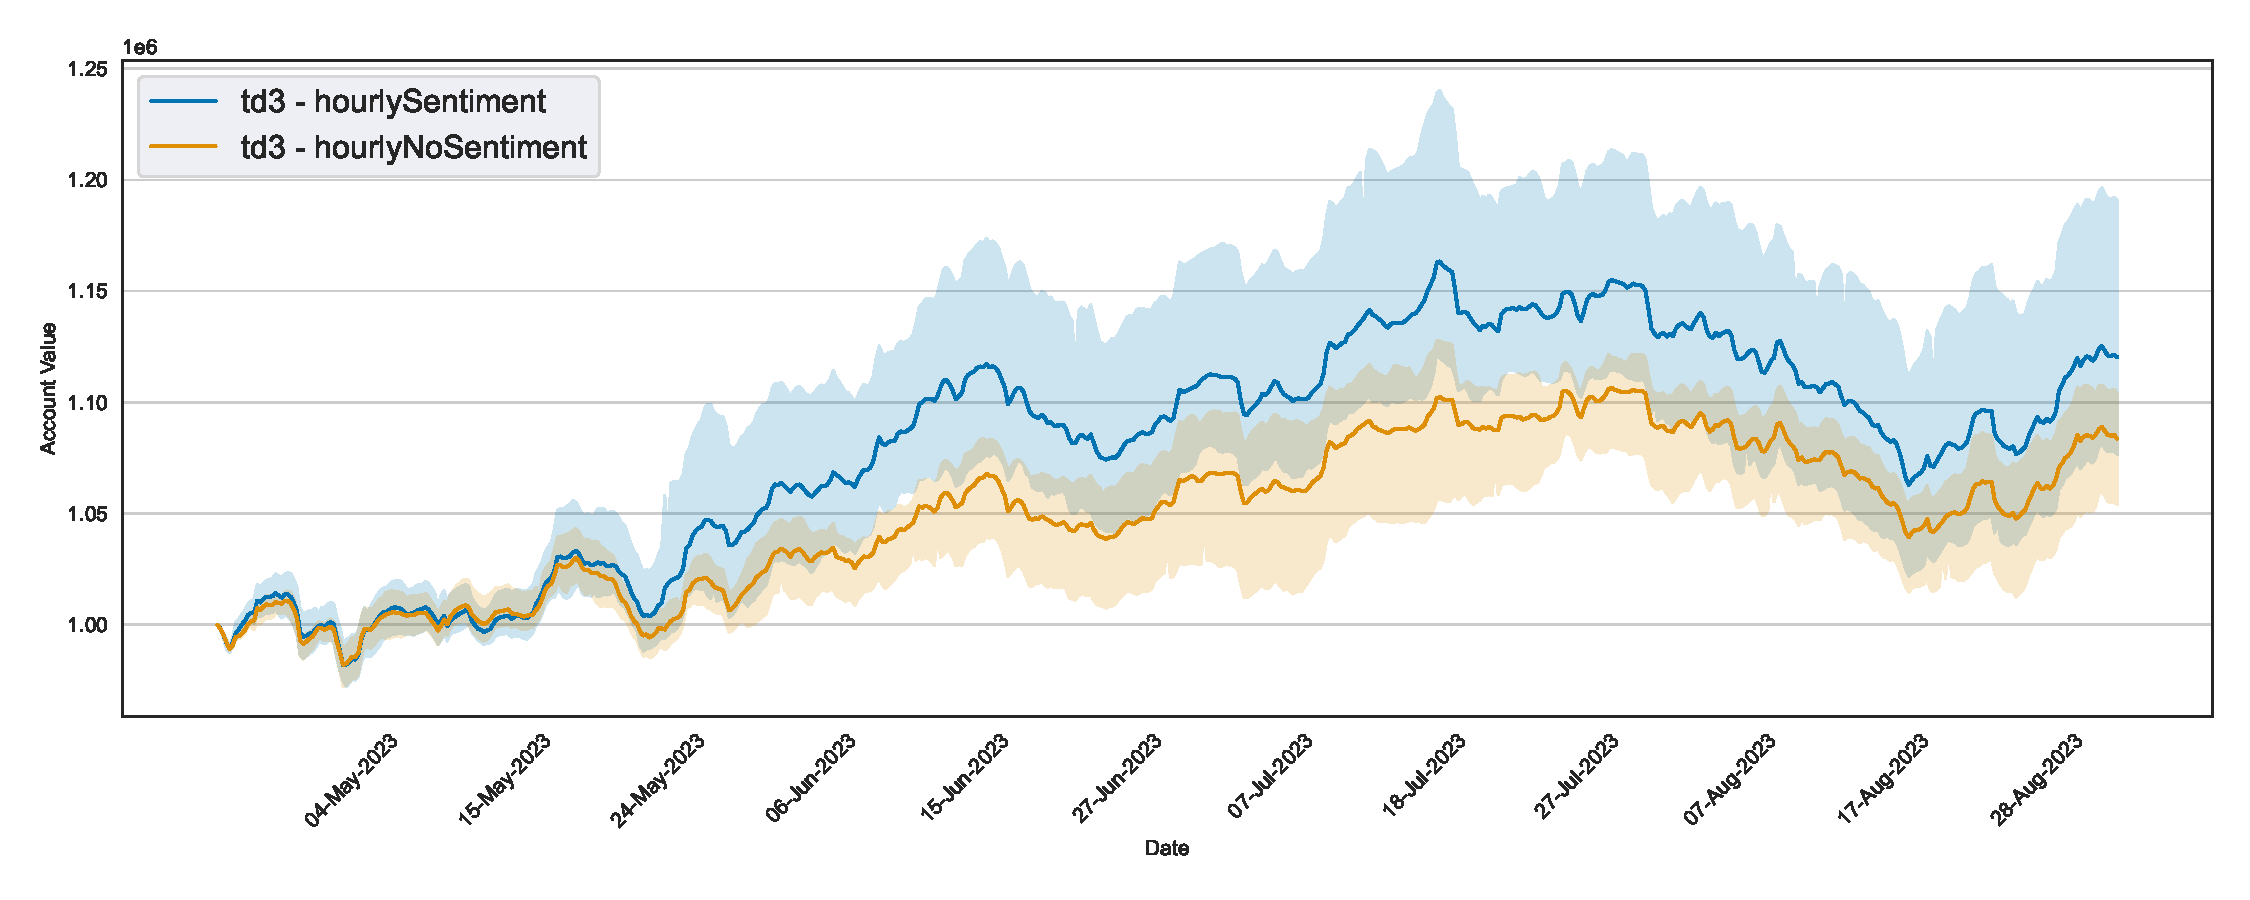
\includegraphics[width=1\textwidth]{figs/Models_comparison/Sentiment/Compare_agent_performance_hourlySentiment_td3.pdf}
\caption{Performance comparison of TD3 agent trained on hourly data with and without sentiment integration.}
\label{fig:Compare_agent_performance_hourlySentiment_td3}
\end{figure}

\begin{figure}[h]
\centering
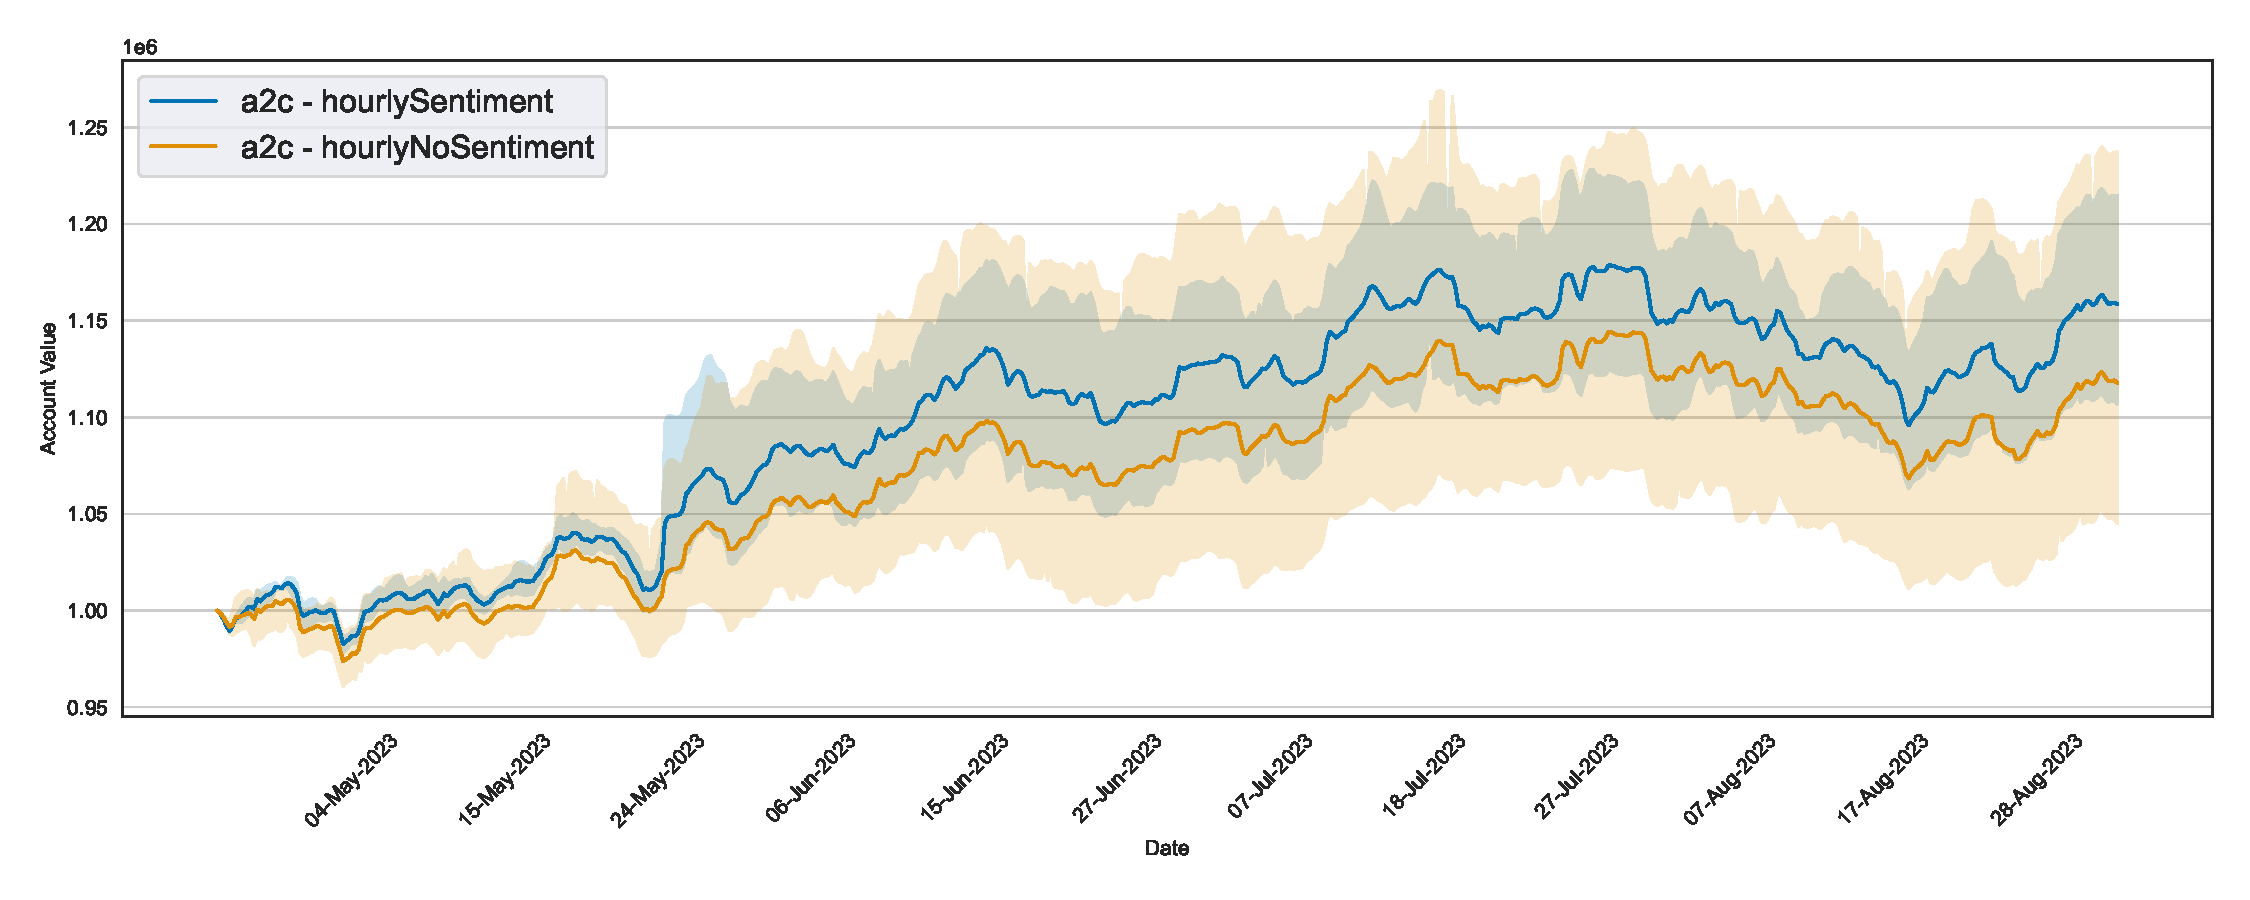
\includegraphics[width=1\textwidth]{figs/Models_comparison/Sentiment/Compare_agent_performance_hourlySentiment_a2c.pdf}
\caption{Performance comparison of A2C agent trained on hourly data with and without sentiment integration.}
\label{fig:Compare_agent_performance_hourlySentiment_a2c}
\end{figure}

\begin{figure}[h]
\centering
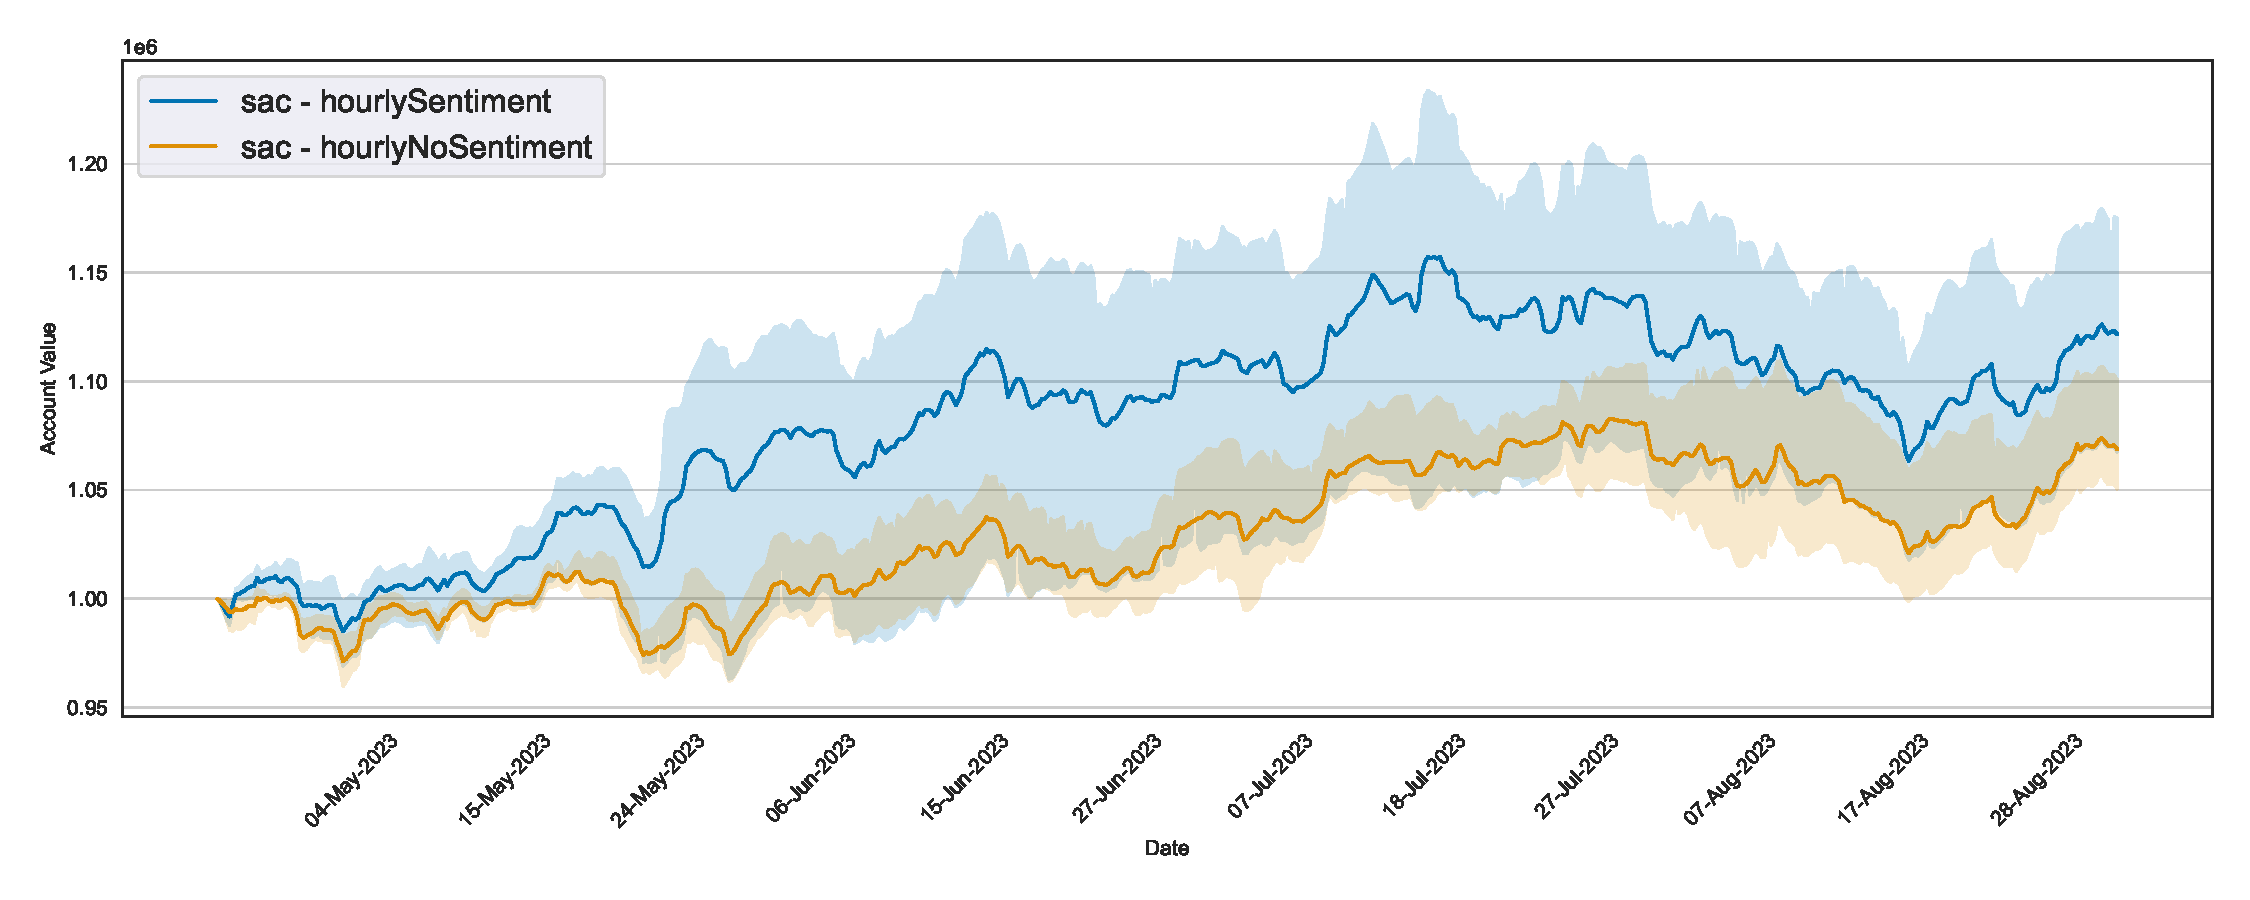
\includegraphics[width=1\textwidth]{figs/Models_comparison/Sentiment/Compare_agent_performance_hourlySentiment_sac.pdf}
\caption{Performance comparison of SAC agent trained on hourly data with and without sentiment integration.}
\label{fig:Compare_agent_performance_hourlySentiment_sac}
\end{figure}





\end{document}
